\section{Kerne- und Elementarteilchen}

Das Verständnis vom Aufbau der Materie basiert auf 4 Schlüsselversuchen der
Kernphysik.
\begin{enumerate}[label=\arabic{*}.)]
\item\emph{Rutherford Streuung} (elastische Streuung).
Rutherford\footnote{Ernest Rutherford, 1. Baron Rutherford of Nelson, OM (* 30.
August 1871 in Brightwater bei Nelson/Neuseeland; † 19. Oktober 1937 in Cambridge)
war ein neuseeländischer, in England wissenschaftlich arbeitender Atomphysiker
und Nobelpreisträger für Chemie des Jahres 1908.} beschoss eine Goldfolie mit
einem dünnen Strahl von Heliumkernen und analysierte die Winkelabhängigkeit.
Zu diesem Zeitpunkt ging man noch davon aus, dass das Atom selbst eine
homogene Ladungsverteilung aufweist. Die Messung zeigte jedoch auch bei großen
Winkeln noch deutliche Streuung, was Rutherford auf einem sehr kleinen
Kerndurchmesser ($\approx 1\mathrm{fm} = 10^{-15}\mathrm{m}$) schließen lies.
Die Formulierung des Rutherfordschen Atommodells revolutionierte die damalige Modellvorstellung.

Präzise elastische Streuversuche liefern Aufschluss über Kerngröße und
Dichteverteilung.
\item \emph{Inelastische Streuung}. Verfeinert man das Experiment der Rutherford
Streuung dahingehend, dass man neben der Winkelablenkung auch die Energie der gestreuten Teilchen misst,
kann man feststellen, welche Anregungszustände ein Kern hat.

Bei höheren Energien, als die bei der Rutherfordstreuung notwendig sind. Stellt
man ähnlich wie in der Optik bei bestimmten Energien Resonanz fest, was darauf
schließen lässt, dass die Protonen bzw. Neutronen eine innere Struktur d.h.
Anregungszustände haben, die auf die Quarks schließen lassen.
\item \emph{Massenspektroskopie}. Wir kennen bereits die
Energie-Masse-Äquivalenz $E=mc^2$. Das heißt aber auch, dass die Masse eines
Teilchens Informationen über seine Bindungen enthält. Dies nutzt man bei der
Massenspektroskopie aus, um durch hochpräzise Massenmessung Informationen über
den Aufbau der Kerne und ihrer Bindungszustände zu erhalten. (Siehe
Literaturaufgabe Übung 3)
\item \emph{Experiment von C.S. Wu}. In den 50ern wurde anhand des
$\beta$-Zerfalls von ${}^{60}Co$ nachgewiesen, dass die Paritätssymmetrie für
die schwache Wechselwirkung gebrochen ist.
\end{enumerate}

\subsection{Rutherford Streuung}
Mitte des 19. Jahrhunderts gab es einen Innovationsschub, der erstmals den
Bau annehmbarer Vakuumpumpen ermöglichte. 1859 konstruierte Plücker die
Gasentladugnsröhre und untersuchte als erster Gasentladungen, gefolgt von
Goldstein 1886.

1897 untersuchte Thomson\footnote{Sir Joseph John Thomson; * 18. Dezember 1856
in Cheetham Hill bei Manchester; † 30. August 1940 in Cambridge) war ein
britischer Physiker und Nobelpreisträger Physik des Jahres 1906}
Kathodenstrahlen $\entspr$ Elektronenstrahlen mit Hilfe der Thomson'schen
Parabelmethode. Dabei verwendete er $E$- und $B$-Felder, um den Strahl
abzulenken.

\rfigure[!htpb][0.45]%
	{2-Parabelmethode.pdf}%
	{\HakenWolf, S. 30}%
	{Prabelmethode, schematische Darstellung. Der durch die Blende $B$
kollimierte Ionenstrahl wird durch den Magneten $M$ und den Kondensator $K$ in
$x$- und $y$-Richtung abgelenkt. Bei größerer Entfernung des Schirms vom
Kondensator werden die Parabeln durch die Projektion entsprechend verzerrt.}
% 
% \begin{SCfigure}[1][!htpb]
% 	\centering
% 	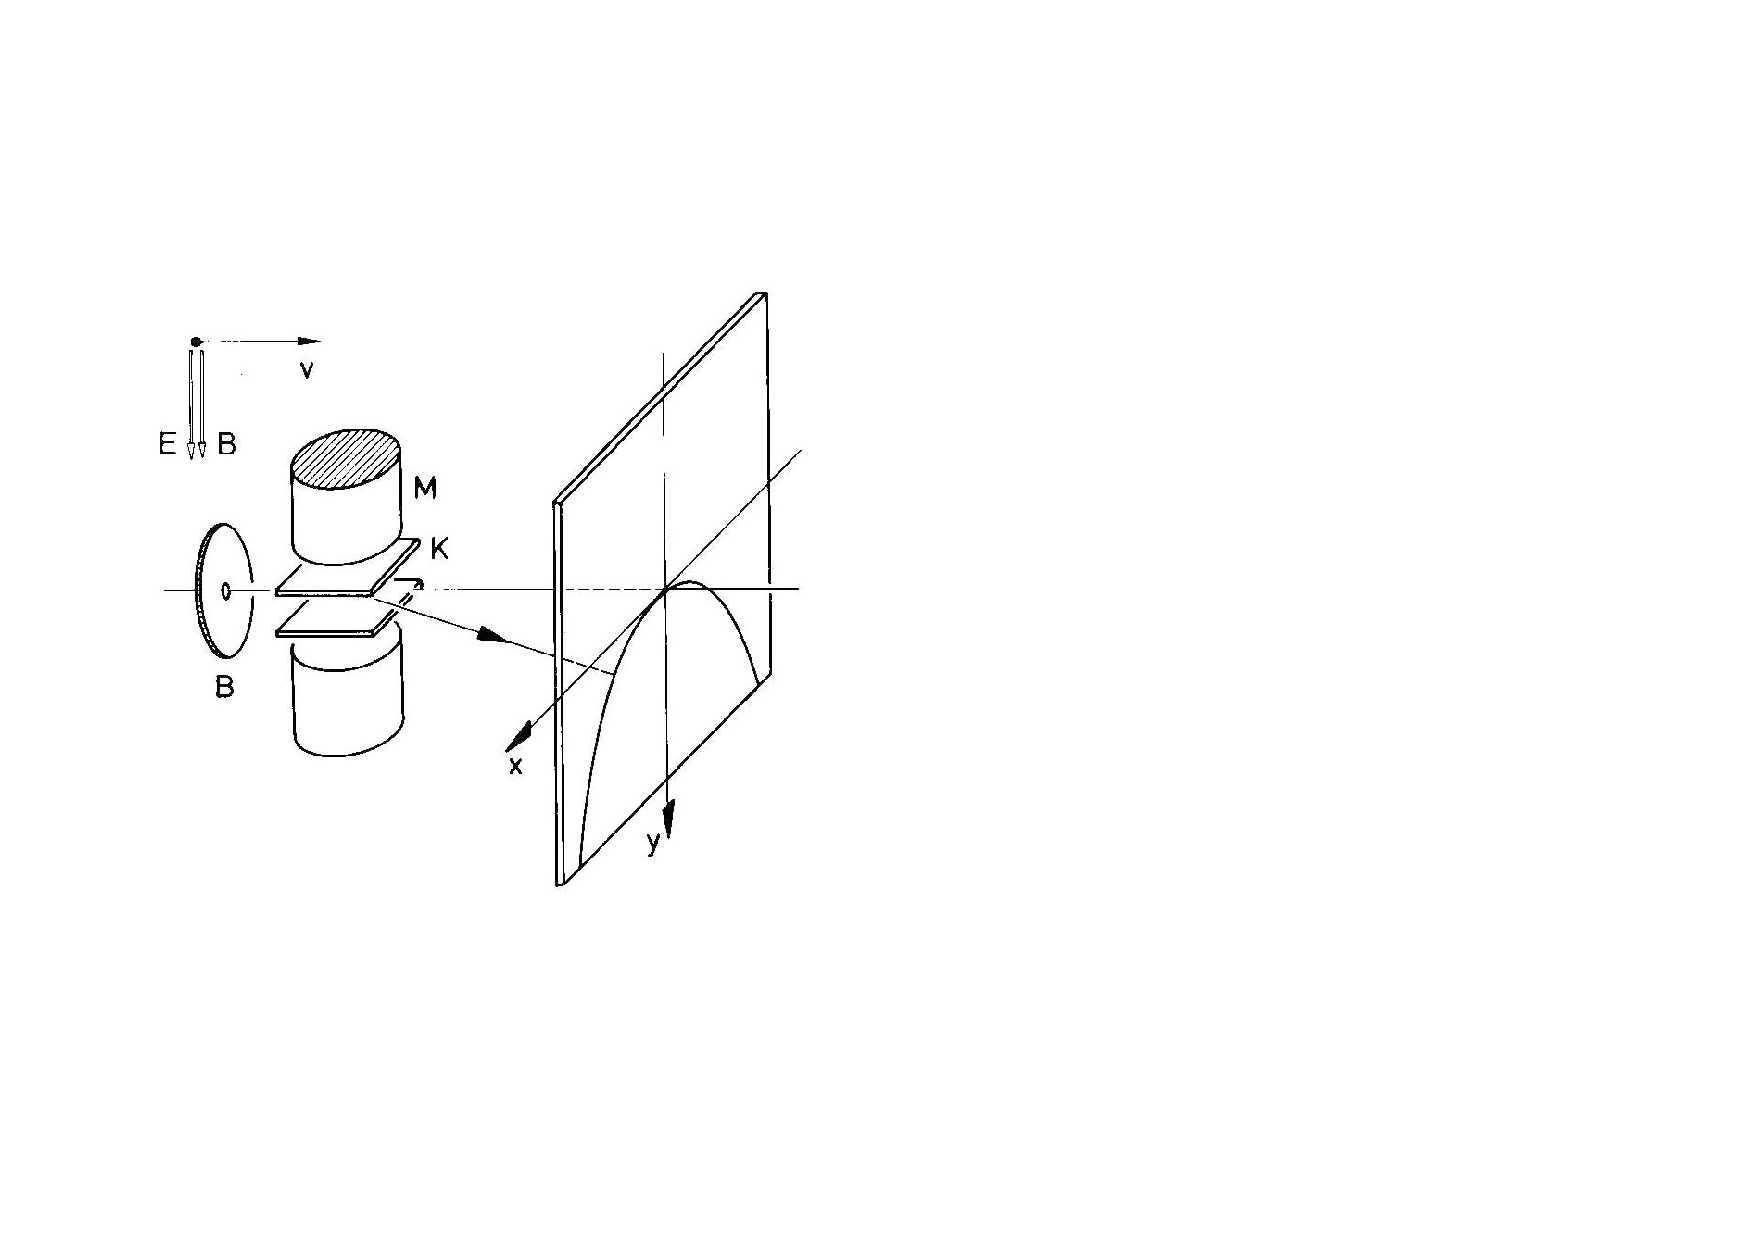
\includegraphics[width=0.5\textwidth]{fig/2-Parabelmethode.pdf}
% \caption{Prabelmethode, schematische Darstellung. Der durch die Blende $B$
% kollimierte Ionenstrahl wird durch den Magneten $M$ und den Kondensator $K$ in
% $x$- und $y$-Richtung abgelenkt. }
% H. Haken, H. C. Wolf, Atom- und Quantenphysik, S. 30 
% \end{SCfigure}
% 
% \begin{figure}[!htbp]
% 	\centering
% 	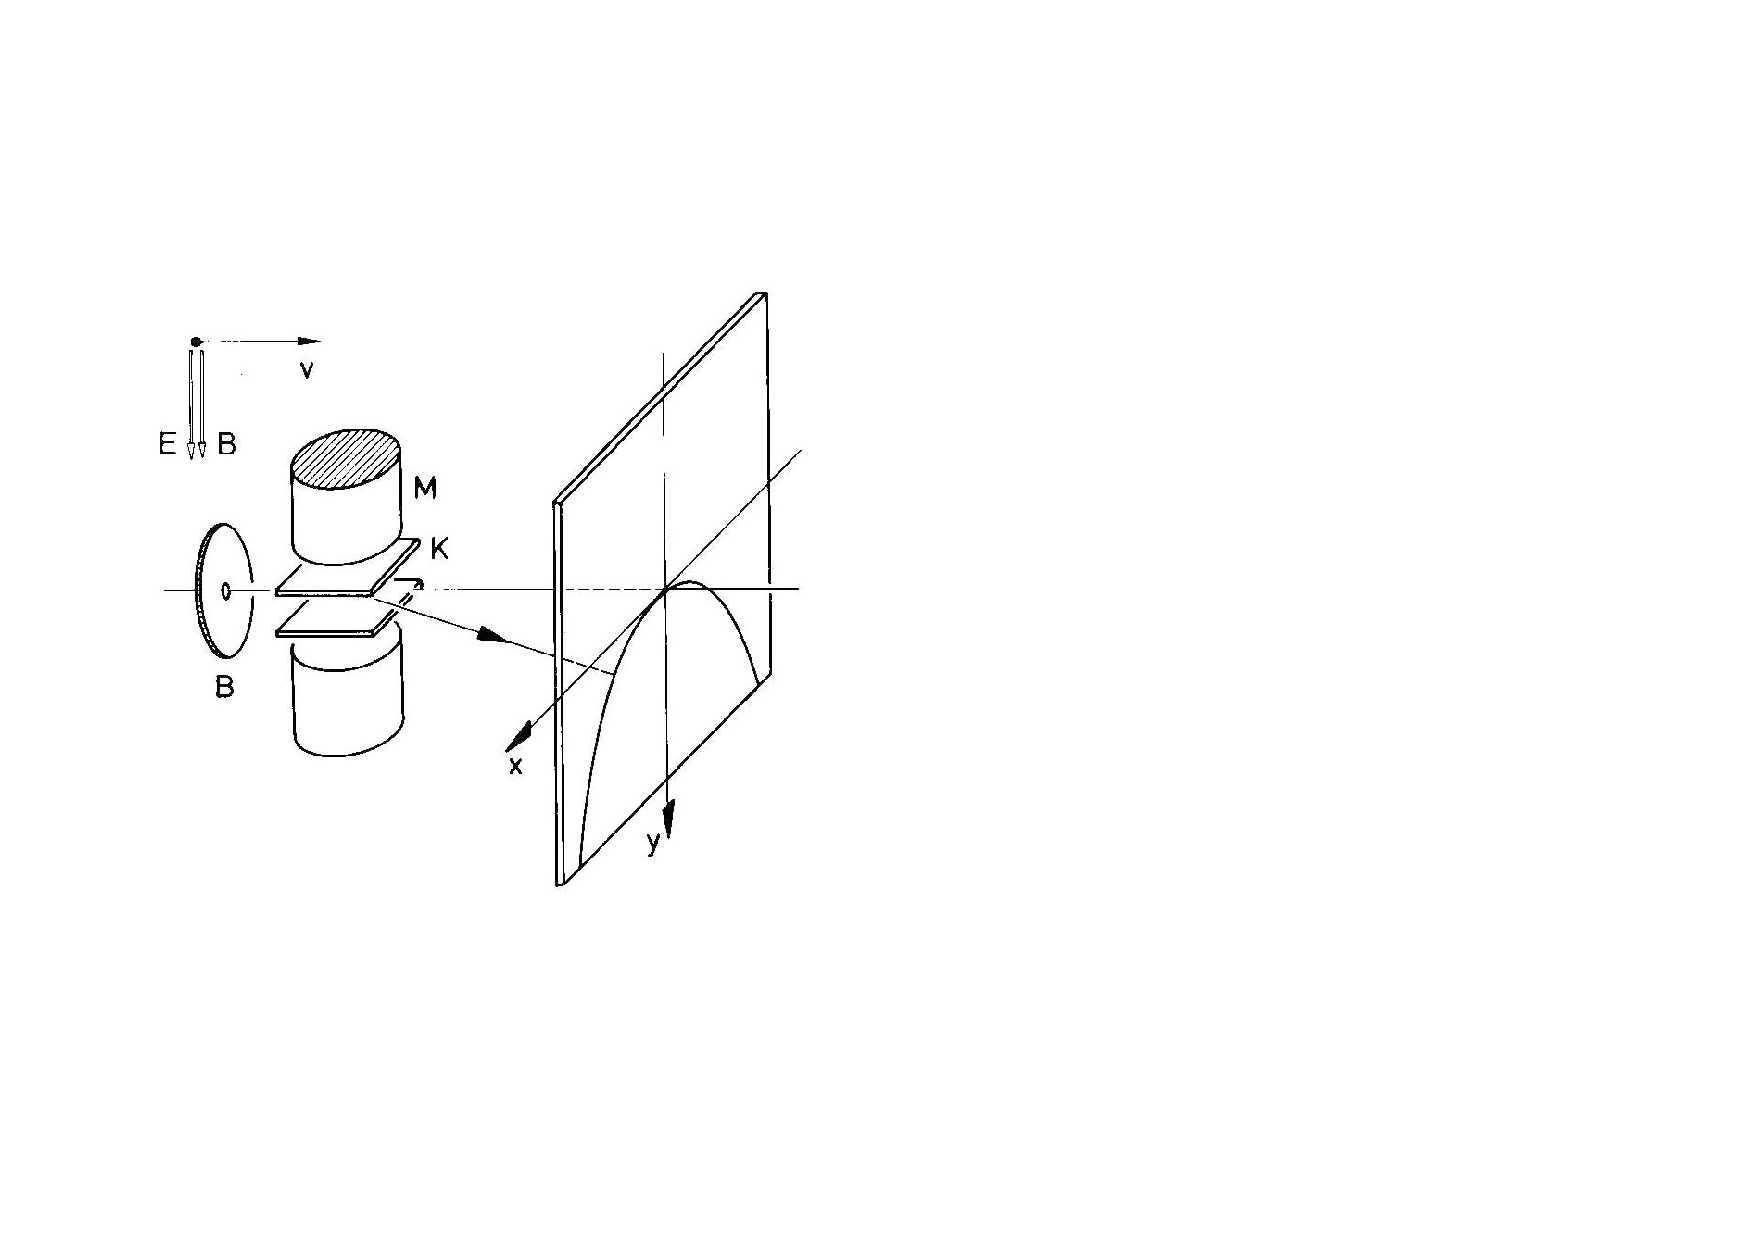
\includegraphics[width=\textwidth]{fig/2-Parabelmethode.pdf}
% \end{figure}

Der Teilchenstrahl durchquert einen Kondensator der Länge $L$, der von einem
Magneten umgeben ist. Elektrisches und Magnetisches Feld zeigen in
$y$-Richtung. Durch das elektrische Feld wirkt auf das Elektron die
Coulombkraft in $y$-Richtung,
\begin{align*}
\vec{F} = e\vec{E} \Rightarrow \ddot{y} = \frac{e}{m}E \Rightarrow y =
\frac{1}{2}\frac{eE}{m}t^2 = \frac{1}{2}\frac{eE}{m}\left(\frac{L}{v}\right)^2
= \frac{eEL^2}{4}\frac{1}{\frac{1}{2}mv^2}\sim \frac{1}{E_{\text{kin}}}\tag{*}
\end{align*}
Daher wird das Elektrische Feld auch ``Energiefilter'' genannt.

Durch das magnetische Feld wirkt auf das Elektron die Lorentzkraft in
$x$-Richtung,
\begin{align*}
&\vec{F} = e(\vec{v}\times\vec{B}) \Rightarrow F_x = evB = F_Z =
\frac{mv^2}{r}\\
\Rightarrow & \text{Kreisbahn mit Radius } r=\frac{mv}{eB}.
\end{align*}
Mit $x<<r$ erhalten wir so
\begin{align*}
a = \frac{evB}{m} \Rightarrow x = \frac{1}{2}at^2 =
\frac{1}{2}\frac{evB}{m}\frac{L^2}{v^2} = \frac{eBL^2}{2}\frac{1}{mv} \sim
\frac{1}{p}.
\end{align*}
Daher wird das magnetische Feld auch ``Impulsfilter'' genannt. Lösen wir den
Term nach $v$ auf und setzen in (*) ein, erhalten wir
\begin{align*}
y = \frac{2E}{L^2B^2}\frac{m}{e}x^2,
\end{align*}
unabhängig von der Geschwindigkeit $v$.

\rfigure[!htpb][0.45]%
	{2-ZerlegungIonenGemisch.pdf}%
	{\HakenWolf, S. 31}%
	{Zerlegung eines Gemisches von Kohlenwasserstoff-Ionen mit der Thomsonschen
	Parabelmethode. Zur Eichung benutzt man Ionen bekannter Masse. Die Intensität
	der einzelnen Parabelstücke entspriccht der relativen Häufigkeit der
	betreffenden Ionen des Gemisches.}

Mit diesem Versuch war auch erstmals die spezifische Ladung messbar,
\begin{align*}
\frac{e}{m} = 1.75\cdot 10^{11} \frac{\mathrm{c}}{\mathrm{kg}}.
\end{align*}

\begin{bemn}
Für große Geschwindigkeiten $v$ (d.h. kleine $x$ und $y$) ergibt sich eine
relativistische Abweichung
\begin{align*}
y = \frac{2E}{L^2B^2}\frac{m}{e}x^2\frac{1}{\sqrt{1-\frac{v^2}{c^2}}}.
\end{align*}
Sie wurde bereits 1902 von Kaufmann\footnote{Walter Kaufmann (* 5. Juni 1871
in Elberfeld; † 1. Januar 1947 in Freiburg im Breisgau) war ein deutscher
Physiker.} beobachtet, jedoch ohne Erklärung.\maphere
\end{bemn}

Kurz darauf (1908) erhielt Rutherford den Nobelpreis für Chemie für die
Entdeckung des $\alpha$-Zerfalls. Die Schwierigkeit hierbei war der Nachweis,
dass $\alpha$-Teilchen in der Tat Heliumkerne sind. Aufgrund ihrer hohen
Geschwindigkeit ließen sie sich durch elektrische Felder nicht maßgeblich
ablenken. Verwendet man jedoch eine Nebelkammer gefüllt mit Helium, sieht man,
dass beim Stoß der $\alpha$-Teilchen mit den Teilchen in der Nebelkammer ein
90° Winkel gebildet wird, d.h. $\alpha$-Teilchen und Helium haben dieselbe
Masse.


\rfigure[!htpb][0.35]%
	{2-Nebelkammer.pdf}%
	{\HakenWolf, S. 43}%
	{Nebelkammer-Aufnahme von $\alpha$-Teilchen. Man sieht Stoßprozesse mit dem
	Füllgas, links mit Wasserstoff, rechts mit Helium. Im Wasserstoff erleidet das
	treffende $\alpha$-Teilchen nur eine geringe Ablenkung, bei Helium dagegen ist
	der Winkel zwischen Bahnen von Streuteilchen und gestoßenem Atom $90^\circ$,
	weil beide die gleiche Masse haben.}

Rutherford verwendete daraufhin in seinen Streuexperimenten $\alpha$-Teilchen,
die er auf eine Goldplatte schoß. Er beobachtete, unter welchem Winkel $\th$
wie viele Ereignisse registriert werden.
\begin{figure}[!htbp]
  \centering
\begin{pspicture}(0,-1.7092611)(6.773818,1.7780532)
\pscircle(1.0171875,0.16){0.37}
\psline[linestyle=dotted,dotsep=0.16cm](1.5671875,0.09)(3.3471875,0.07)
\psline(3.6,0.15)(3.6,1.57)
\psline(3.6,-0.01)(3.6,-1.37)
\psline{->}(3.6871874,0.07)(4.5871873,0.07)
\psline[linestyle=dotted,dotsep=0.16cm](1.5671875,0.41)(3.2471876,1.09)
\psline[linestyle=dotted,dotsep=0.16cm](1.5471874,-0.19)(3.1671875,-0.83)
\psline[linecolor=yellow](4.7871876,0.79)(4.7671876,-0.47)
\psline[linestyle=dotted,dotsep=0.16cm](4.8671875,0.07)(6.5471873,0.07)
\psarc(5,0.08){0.53}{0}{50}
\psline[linecolor=darkblue]{->}(4.8871875,0.15)(6.1471877,1.07)
\psarc(4.6,0.0){1.97}{300.96375}{63.17802}

\rput{36.360546}(2.0732305,-3.5930915){\psframe[linewidth=0.04,dimen=outer](6.7671876,1.47)(6.2471876,1.25)}

\rput(1.0,-0.75){Quelle: Radon}
\rput(4.7,-0.75){Target}
\rput(3.6,-1.58){Blende}

\rput(2.6,0.32){\color{gdarkgray}$\alpha^{++}$}
\rput(5.3,0.25){\color{gdarkgray}$\th$}
\end{pspicture} 
  \caption{Versuchsaufbau: Rutherfordstreuung.}
\end{figure}


Zum Zeitpunkt der Durchführung des Experiments ging man noch vom
Thomsonschen Atommodell aus.
\begin{enumerate}[label=\arabic{*}.)]
  \item Elektronen sind in allen Elementen enthalten.
  \item Die Ladungsverteilung im Atom ist homogen, Protonen, Neutronen und
  Elektronen verteilen sich so, dass die elektrostatische Anziehung minimiert
  wird.
\end{enumerate}

\sfigure[!htpb]%
	{2-AtommodellThomson.pdf}
	{}
	{Das Elektron als elementarer Baustein der Materie.}

Rutherford stellte in seinem Versuch jedoch auch bei großen Winkeln $\th>90°$
noch Ablenkung fest, was darauf schließen ließ, dass der Atomkern
einen viel kleineren Radius als das Atom selbst haben muss.

\begin{figure}[!htbp]
	\centering
	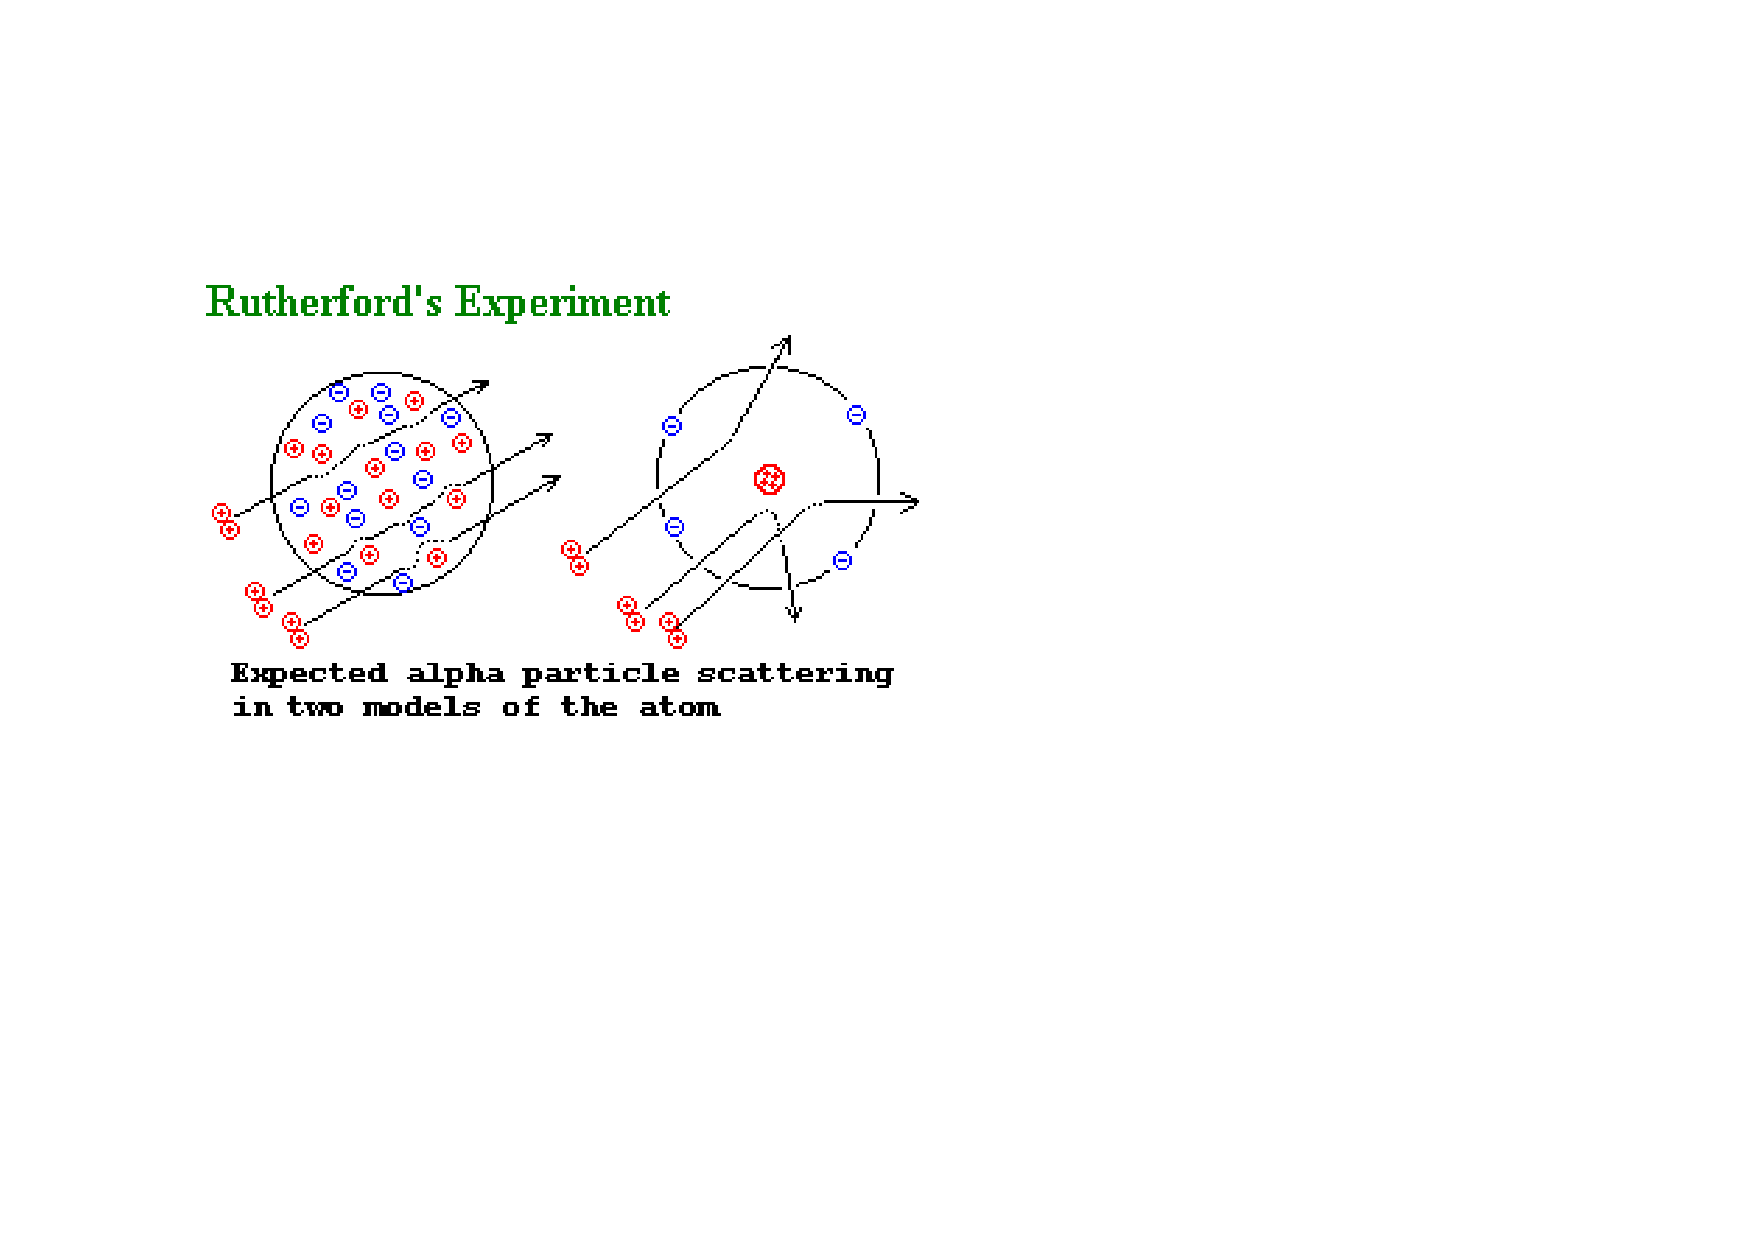
\includegraphics[width=0.49\textwidth]{fig/2-RutherfordStreuungErwartung.pdf}
	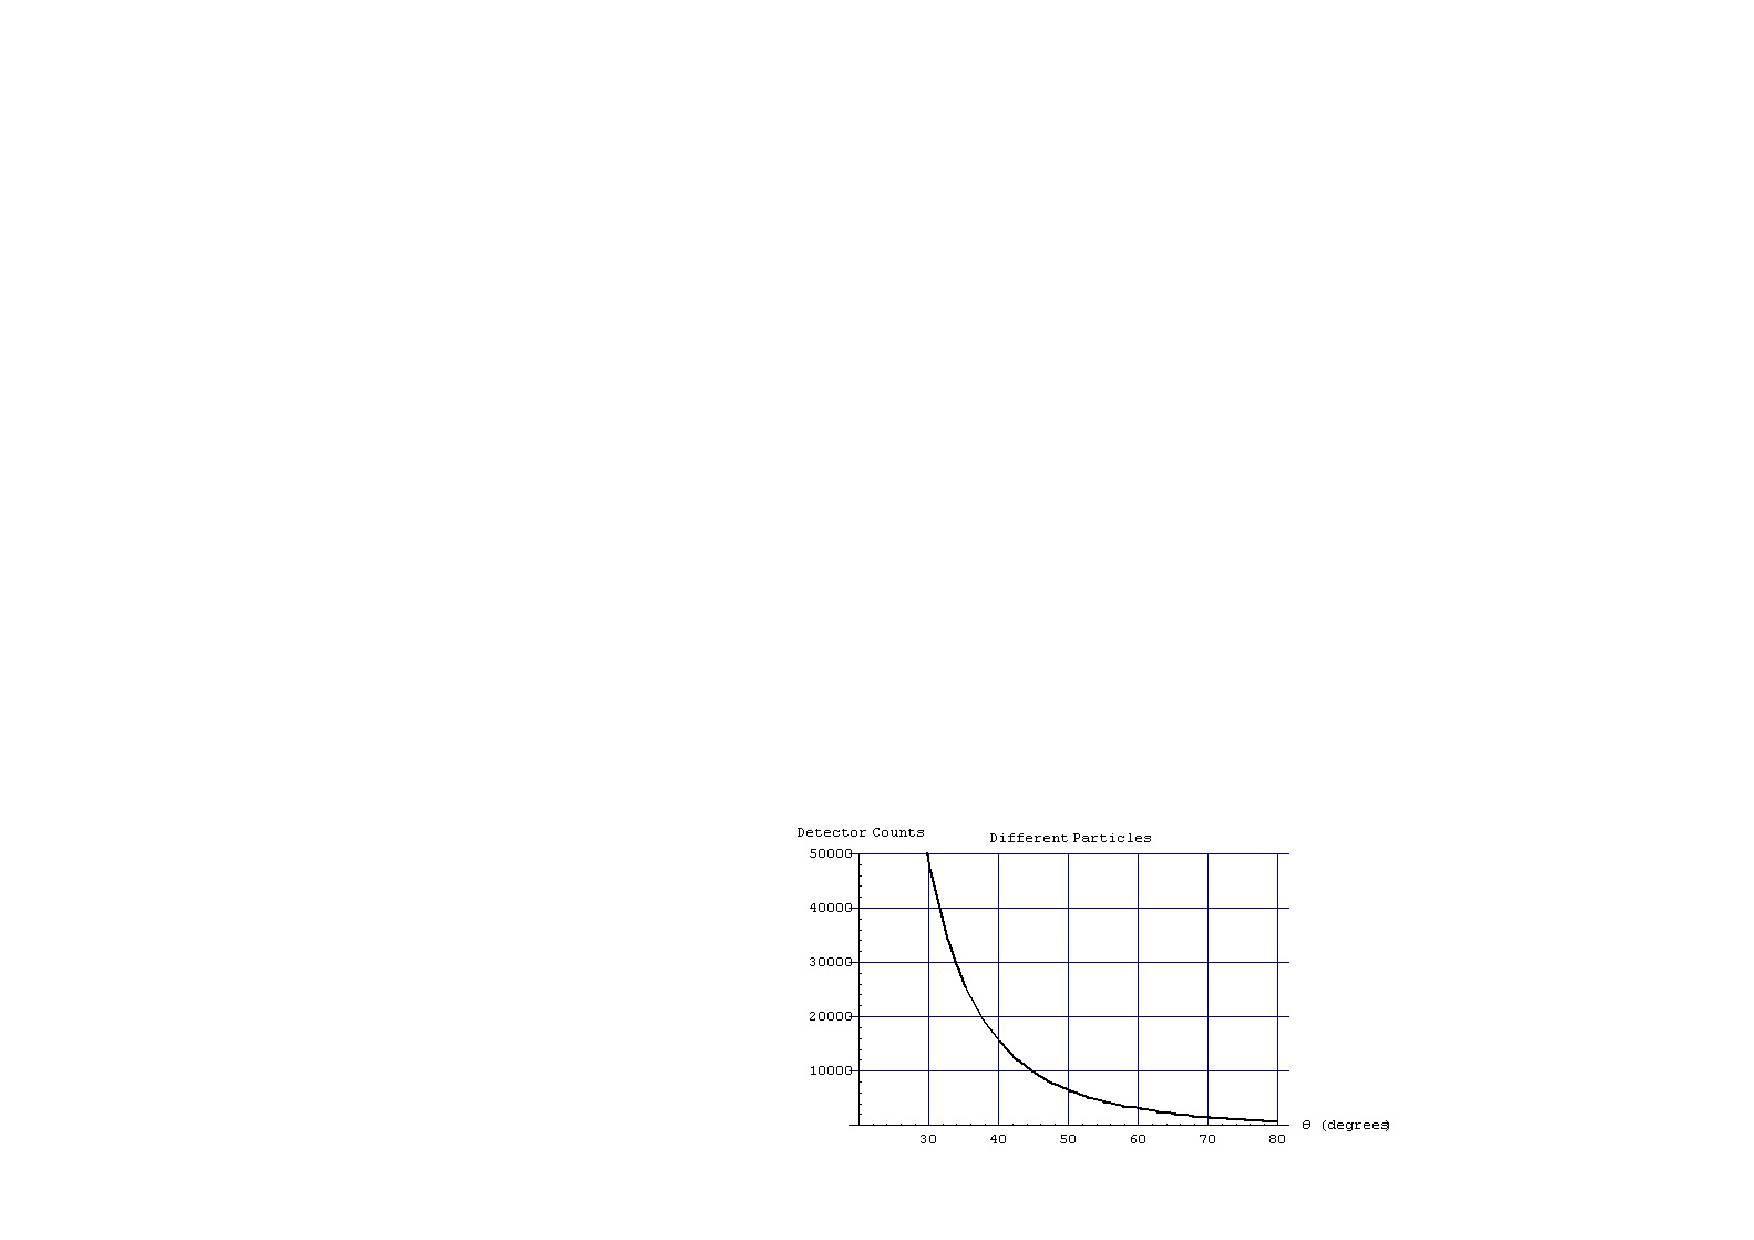
\includegraphics[width=0.49\textwidth]{fig/2-RutherfordExperimentWinkelabhaengigkeit.pdf}
	\caption{Modellvorstellungen zur $\alpha$-Teilchen Streuung (links) und real
	gemessene Intensität in Abhängigkeit vom Winkel (rechts).}
\end{figure}

\begin{figure}[!htbp]
	\centering
	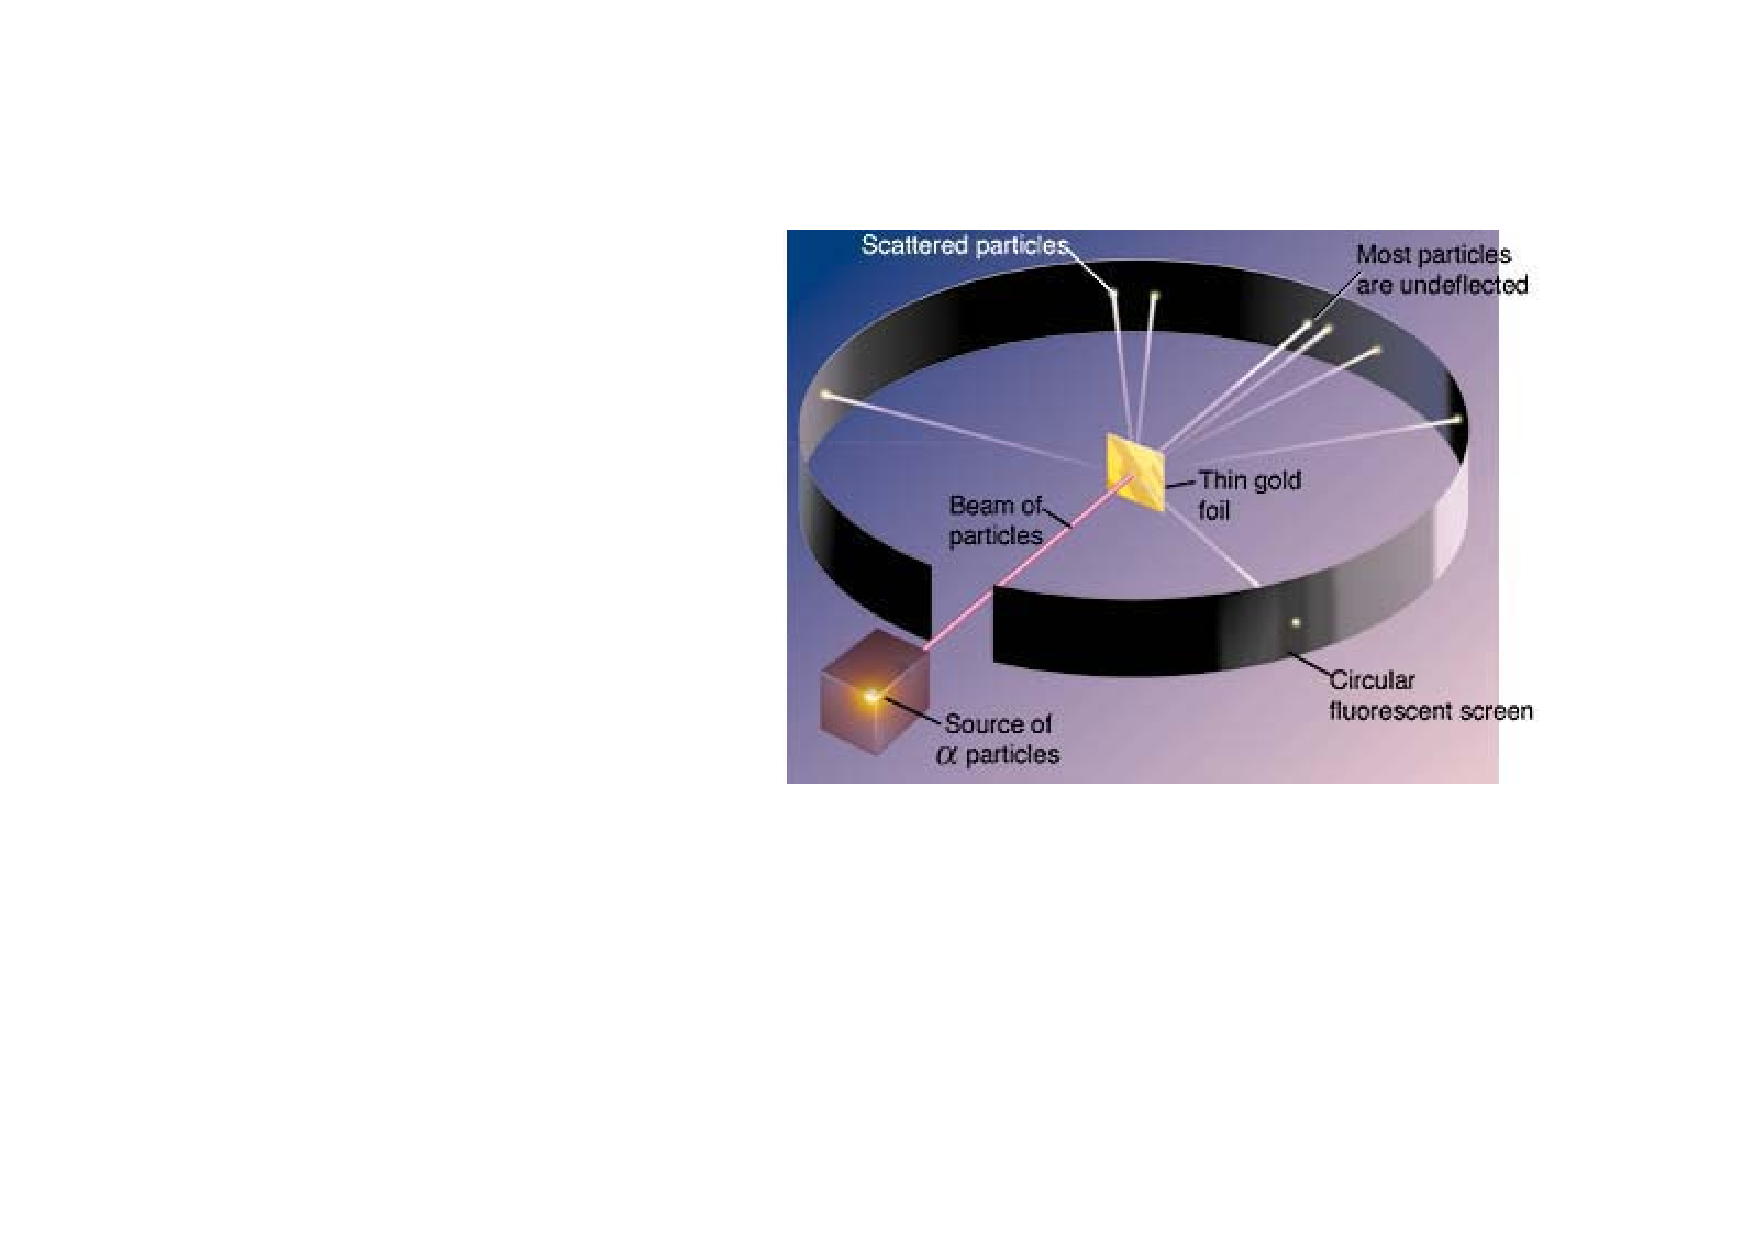
\includegraphics[width=\textwidth]{fig/2-RutherfordExperimentAufbau.pdf}
\end{figure}

\subsubsection{Rutherford'sche Streuformel}
	
Um die Ergebnisse zu formulieren benötigen wir noch einige Begriffe.
\begin{defnn}
Der \emph{Wirkungsquerschnitt} $\sigma$ ist ein Maß für die Wahrscheinlichkeit
einer Reaktion. Die Zahl der Rekationen ist gegeben durch,
\begin{align*}
N = j\cdot n\cdot\sigma,
\end{align*}
wobei $j$ die Stromdichte der einfallenden Teilchen und $n$ die Zahl der
Targetteilchen bezeichnet. $\sigma$ hat hier die Einheit einer Fläche.\fishhere
\end{defnn}

Wir sehen, dass $\sigma$ die relevanten Informationen über die
einzelnen Reaktionen enthält.

\begin{bemn}
Für ein Target aus Kugelteilchen ist $\sigma = \pi R^2$. Bei Coulomb-Stößen
geht jedoch die geometrische Anschauung verloren, denn die Wechselwirkung hat
$\infty$-Reichweite. D.h. der Wirkungsquerschnitt divergiert im Raum. Man geht
daher zu differentiellen Größen über,
\begin{align*}
\dot{N}(\th) = j\cdot n\cdot\sigma(\th)\Delta\Omega,
\end{align*}
wobei $\sigma$ hier einen differentiellen Wirkungsquerschnitt bezeichnet und
$\Delta \Omega$ einen Raumwinkel.\maphere
\end{bemn}

\sfigure[htbp][0.6]%
	{2-DefinitionDifferentiellerWirkungsquerschnitt.pdf}%
	{}
	{Zur Definition des differentiellen Wirkungsquerschnitts.}

Rutherford hat die Winkelabhängigkeit des differentiellen Wirkungsquerschnitts
empirisch bestimmt. Um den Ausdruck für $\sigma$ theoretisch herzuleiten,
verwendet man Drehimpulserhaltung,
\begin{align*}
&\vec{L} = \mu \left(\vec{r}\times\vec{v}\right) = \const,\tag{*}\\
\Rightarrow & \abs{\vec{L}} = \mu r^2 \frac{\diffd \ph}{\dt} = \mu v_0 b,
\end{align*}
sowie Impulserhaltung,
\begin{align*}
\abs{\vec{p}} = m v_0 = \const.
\end{align*}

\sfigure[H]%
	{2-SkizzeRutherfordStreuformel.pdf}%
	{}
	{Zur Herleitung der Winkelabhängigkeit.}

Die Bewegung findet nur in der $x,y$-Ebene statt, welche $\bot$ zu $\vec{L}$
ist. Setze $a:= \frac{Z_1Z_2 e^2}{4\pi\ep_0}$ und berechne $p_y$,
\begin{align*}
\dot{v}_y &= \frac{1}{\mu} F_y = \frac{1}{\mu}\frac{a}{r^2}\sin\ph
\overset{*}{=} \frac{1}{\mu}a\sin\ph \frac{\dph}{\dt}\frac{1}{v_0 b}.\\
\Rightarrow 
v_y &= \int\limits_{-\infty}^\infty \dot{v}_y \dt = \int\limits_{0}^{v_0\sin\th}
\diffd v_y = v_0\sin\th
= \frac{a}{\mu v_0 b}\int\limits_{-\infty}^\infty \sin\ph \frac{\dph}{\dt}\dt\\
&= \frac{a}{\mu v_0 b}\int\limits_{0}^{\pi-\th} \sin\ph \dph
= \frac{a}{\mu v_0 b}(1+\cos\th).
\end{align*}
Wir erhalten somit,
\begin{align*}
\cot \frac{\th}{2} = 
\frac{1+\cos\th}{\sin\th}=
\mu v_0^2\frac{b}{a} = 2 E_0 \frac{b}{a} = 2 \frac{E_0}{V_\text{pot}(b)},
\end{align*}
d.h. wir können $\th$ in Abhängigkeit von $b$ darstellen. Invertieren ergibt,
\begin{align*}
b(\th) = \frac{D}{2}\cot\frac{\th}{2},\qquad D=\frac{1}{4\pi\ep_0}\frac{Z_1Z_2e^2}{E_0}.
\end{align*}
Mit $\sigma(\th) = \frac{b}{\sin\th}\abs{\frac{\db}{\dth}}$ erhalten wir so für
den differentiellen Wirkungsquerschnitt,
\begin{align*}
\sigma(\th) =
\left(\frac{D}{4}\right)^2\frac{1}{\sin^4\left(\frac{\th}{2}\right)}.
\end{align*}
Die $\sin^{-4}\left(\frac{\th}{2}\right)$ Proportionalität ist
charakteristisch für die Rutherford Streuung.

Im Streuexperiment erwartet man also
\begin{align*}
N(\th) = j\cdot n \cdot C \cdot \Delta\Omega
\sin^{-4}\left(\frac{\th}{2}\right).
\end{align*}
Mithilfe von $C$ kann man $\frac{Z_1Z_2}{E_0}$ bestimmen.

\subsubsection{Kernradienbestimmung}
Bei der Messung von $\sigma$ wird in der Regel der Winkel $\th$ variiert unter
dem der Detektor misst. In großen Beschleunigeranlagen kann man auch den Winkel
konstant halten und die kinetische Energie variieren, um die
$\frac{1}{E_\text{kin}}$-Abhängigkeit zu verifizieren. Die Formel für den
differentiellen Wirkungsquerschnitt wurde experimentell für
\begin{align*}
E_\text{kin} < 5MeV,\qquad \th<150°,
\end{align*}
bestätigt. Für den Stoßparameter $b$ gilt,
\begin{align*}
b(\th) = \frac{D}{2}\cot\frac{\th}{2} < 6\cdot 10^{-15}m.
\end{align*}
Wir erhalten so eine obere Grenze für den Kernradius.
\begin{align*}
R \approx r_0\cdot A^{1/3},\qquad r_0 = 1.3\cdot 10^{-15}m,
\end{align*}
wobei $A$ für die Nukleonenzahl steht. Der Kerndurchmesser liegt also im
Femtometerbereich und damit $5$ Größenordnungen unter dem Atomdurchmesser.
Außerdem sehen wir, dass bei großer Entfernung vom Kern das Potential gerade
wie ein Coulomb-Potential aussieht.

\rfigure[!htpb][0.4]%
	{2-KernCoulomb.pdf}%
	{\HakenWolf, S. 49}%
	{Kernkraft- und Coulombpotential.}

Wir wollen nun untersuchen, wie wir durch Messungen von
$\frac{\diffd\sigma}{\diffd\Omega}$ Aussagen über die Form des Potentials machen
können.

\rfigure[!htpb][0.4]%
	{2-StreuungAlphaElast.pdf}%
	{\FrauenfelderHenley, S. 171}%
	{Differentieller Wirkungsquerschnitt für die elastische Streuung von
	$\alpha$-Teilchen an ${}^{24}Mg$.}

% \begin{figure}[!htbp]
% 	\centering
% 	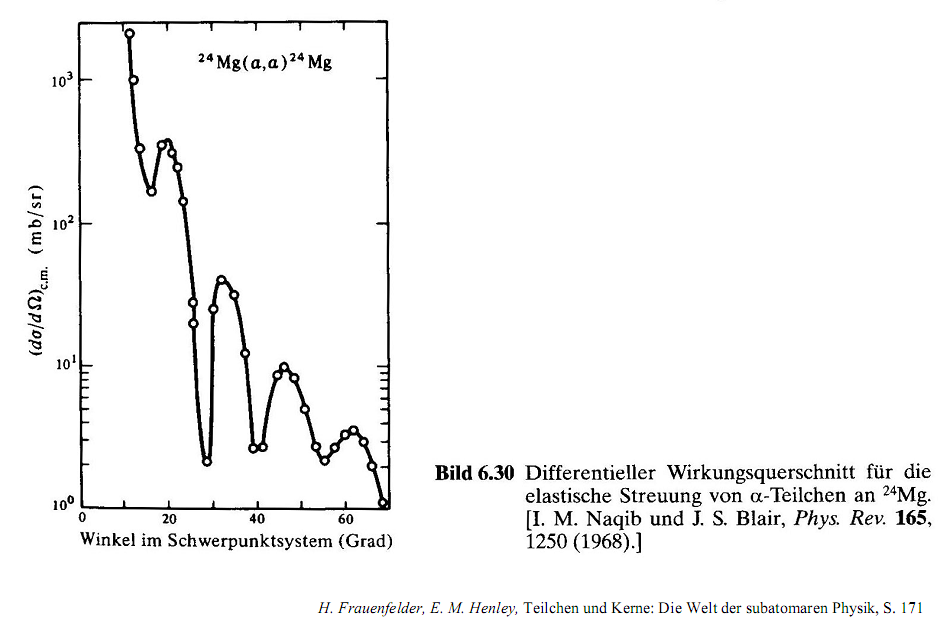
\includegraphics[width=\textwidth]{fig/2-StreuungAlphaElast.png}
% \end{figure}
Ähnlich wie bei Beugungsexperimenten in der Optik, tritt für bestimmte Winkel
$\th$ Resonanz im Kern auf und wir erhalten Beugungsmaxima. Verwenden wir verschiedene Teilchen als
Streuteilchen, erhalten wir Informationen über die verschiedenen
Wechselwirkungen (stark, schwach, elektromagnetisch).

Für geladene Streuteilchen muss die Energie hoch genug sein, um den Kern selbst
zu erreichen und zu untersuchen. Um Details im Kern aufzulösen, muss aber auch
ein neutrales Streuteilchen genug Energie haben. Im Bild der Optik muss die de
Broglie Wellenlänge des Streuteilchens viel kleiner sein als der Kern, um die
detailierte Struktur zu ``mikroskopieren''.
\begin{bspn}
\begin{enumerate}[label=\arabic{*}.)]
  \item Neutronen erfahren keine Coulomb Wechselwirkung. Das Beugungsmuster
  kommt nur durch starke Wechselwirkung zustande.

\rfigure[!htpb][0.5]%
	{2-StreuungNeutronenElast.pdf}%
	{\Stierstadt, S. 91}%
	{Winkelverteilung von an Atomkernen gestreuten Neutronen mit $2.2\cdot
	10^{-12}\mathrm{J} (14\mathrm{MeV})$ Primärenergie. Die durchgezogenen Kurven
	sind mit dem Modell berechnet.}

% \begin{figure}[!htbp]
% 	\centering
% 	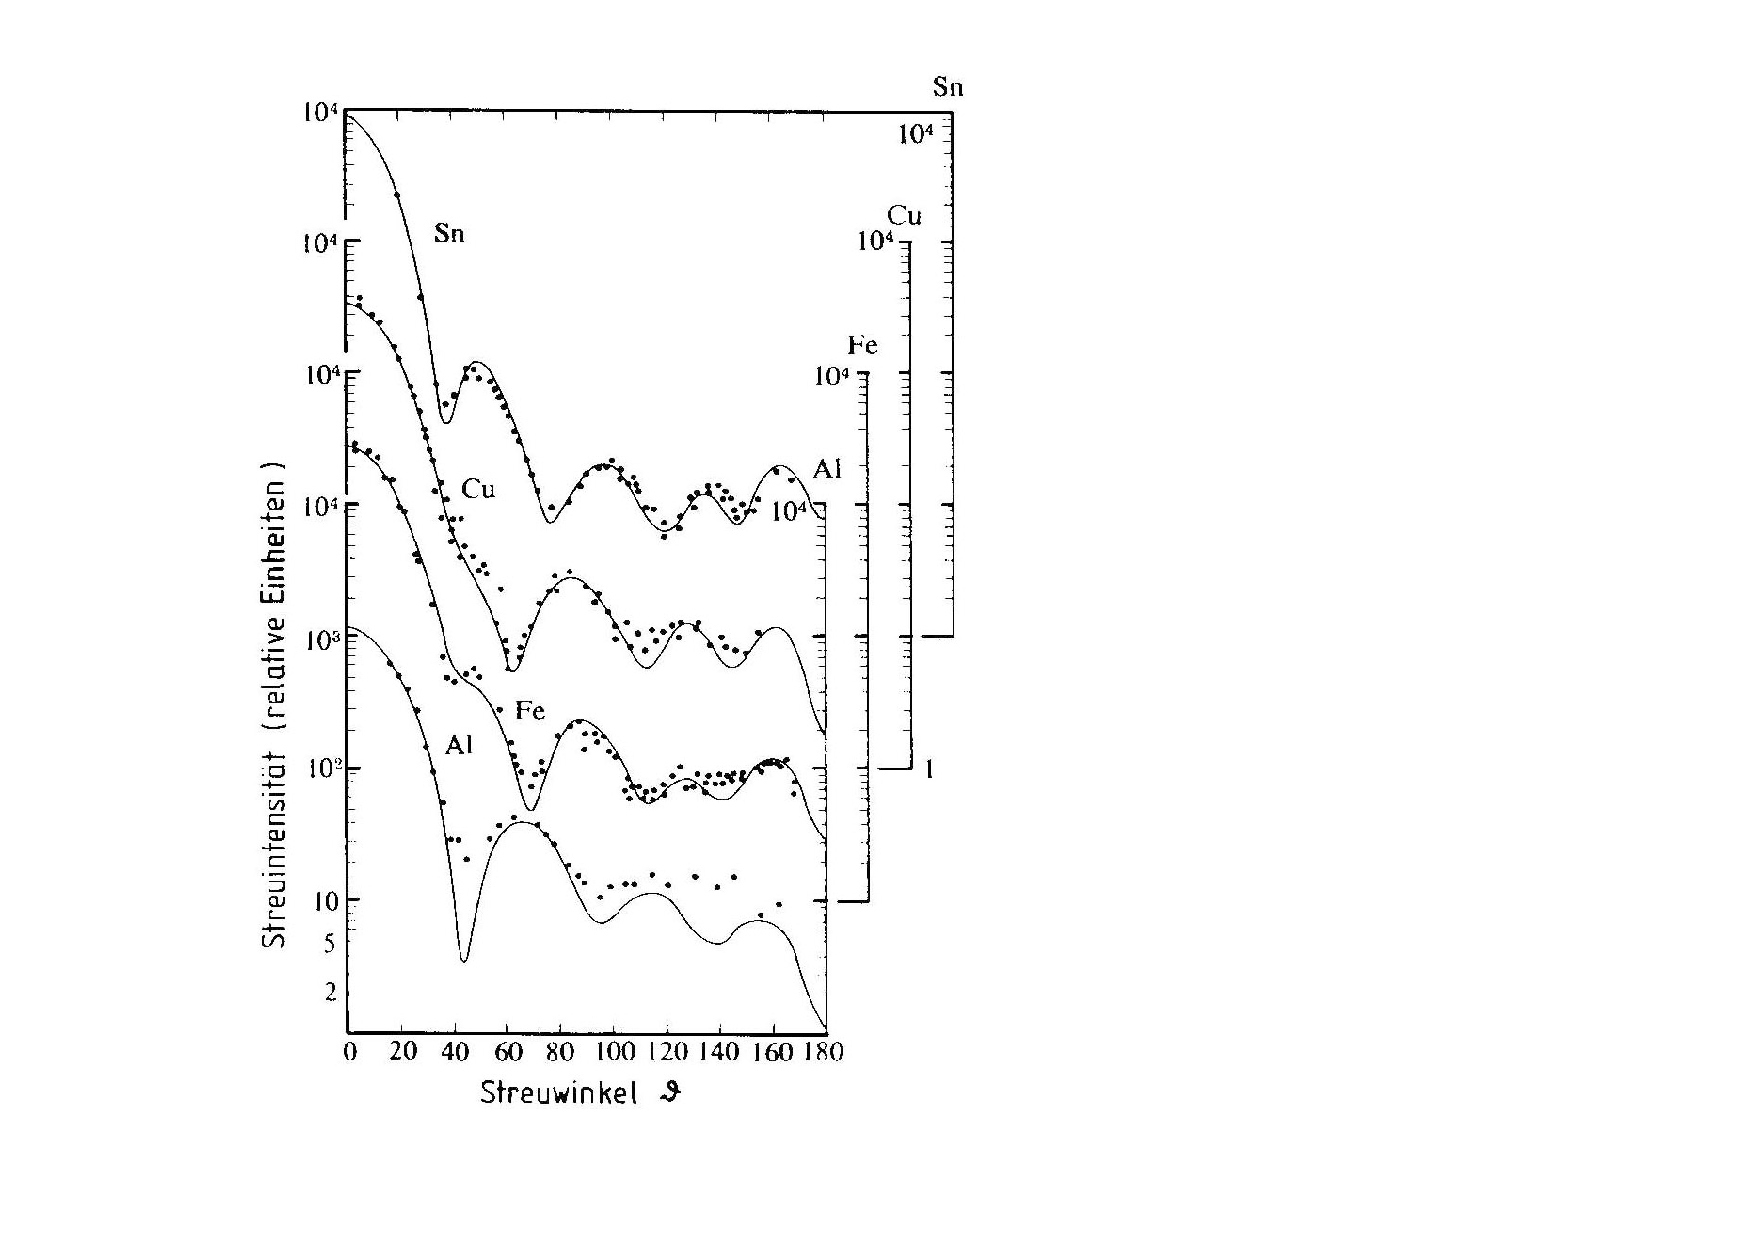
\includegraphics[width=\textwidth]{fig/2-StreuungNeutronenElast.pdf}
% \end{figure}
\item Elektronen erfahren nur Coulomb-Wechselwirkung.
\rfigure[!htpb][0.4]%
	{2-StreuungElektronElast.pdf}%
	{\KuckukKern, S. 27}%
	{Winkelverteilung elastisch gestreuter Elektronen an Kohlenstoff.}
\rfigure[!htpb][0.5]%
	{2-StreuungElektron2Elast.pdf}%
	{\BethgeWalter, S. 42}%
	{Elektronenstreuung an Uran, gemessen bei zwei Energien.}

% \begin{figure}[!htbp]
% 	\centering
% 	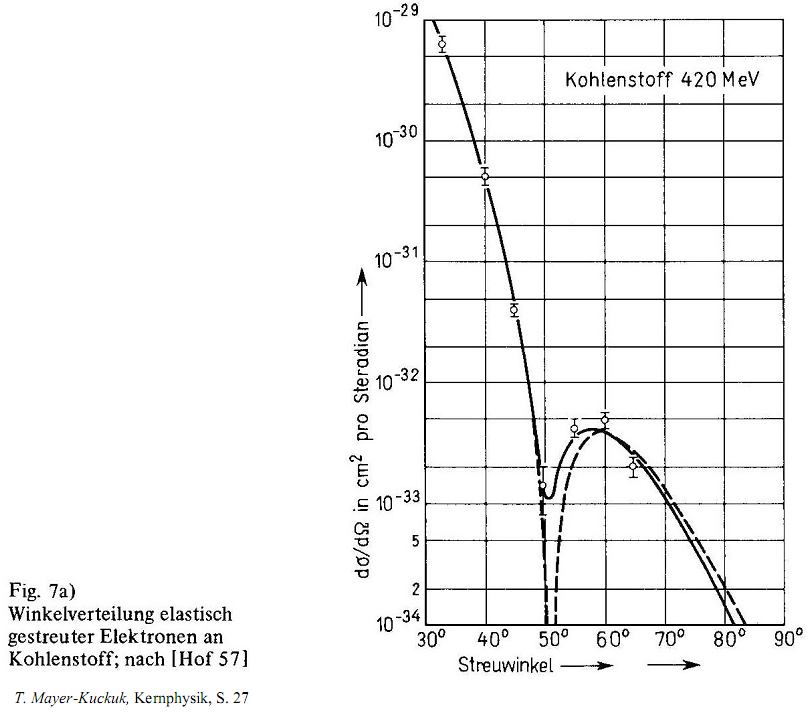
\includegraphics[width=\textwidth]{fig/2-StreuungElektronElast.png}
% \end{figure}
% \begin{figure}[!htbp]
% 	\centering
% 	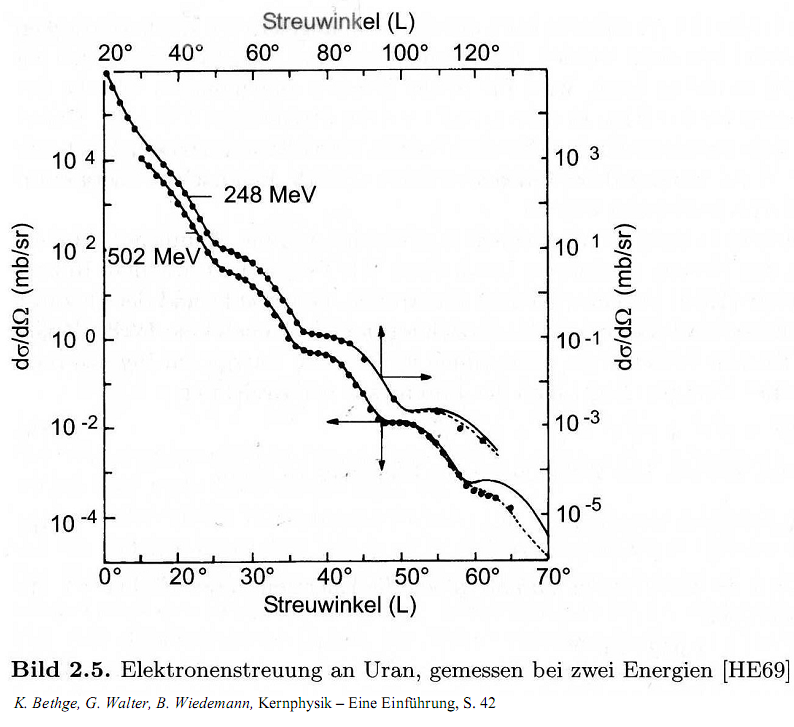
\includegraphics[width=\textwidth]{fig/2-StreuungElektron2Elast.png}
% \end{figure}
\item Die Messergebnisse zeigen, dass die Ladungsverteilung von der
Atommasse abhängt. Ist das Wasserstoffatom noch singulär, so hat Silizium
eine homogene Dichteverteilung. Schwere Kerne haben in etwa alle die gleiche
homogene Kerndichte.

\sfigure[!htpb]%
	{2-StreuungLadungsvert.pdf}%
	{\BethgeWalter, S. 44}%
	{\label{fig:radlad}Radiale Ladungsverteilungen einiger Atomkerne. Diese Daten
	werden aus der Inversion der Streudaten gewonnen, ähnlich wie man aus dem
	Fernfeldbeugungsbild in der Optik das beugende Objekt rekonstruieren kann.}

% \begin{figure}[!htbp]
% 	\centering
% 	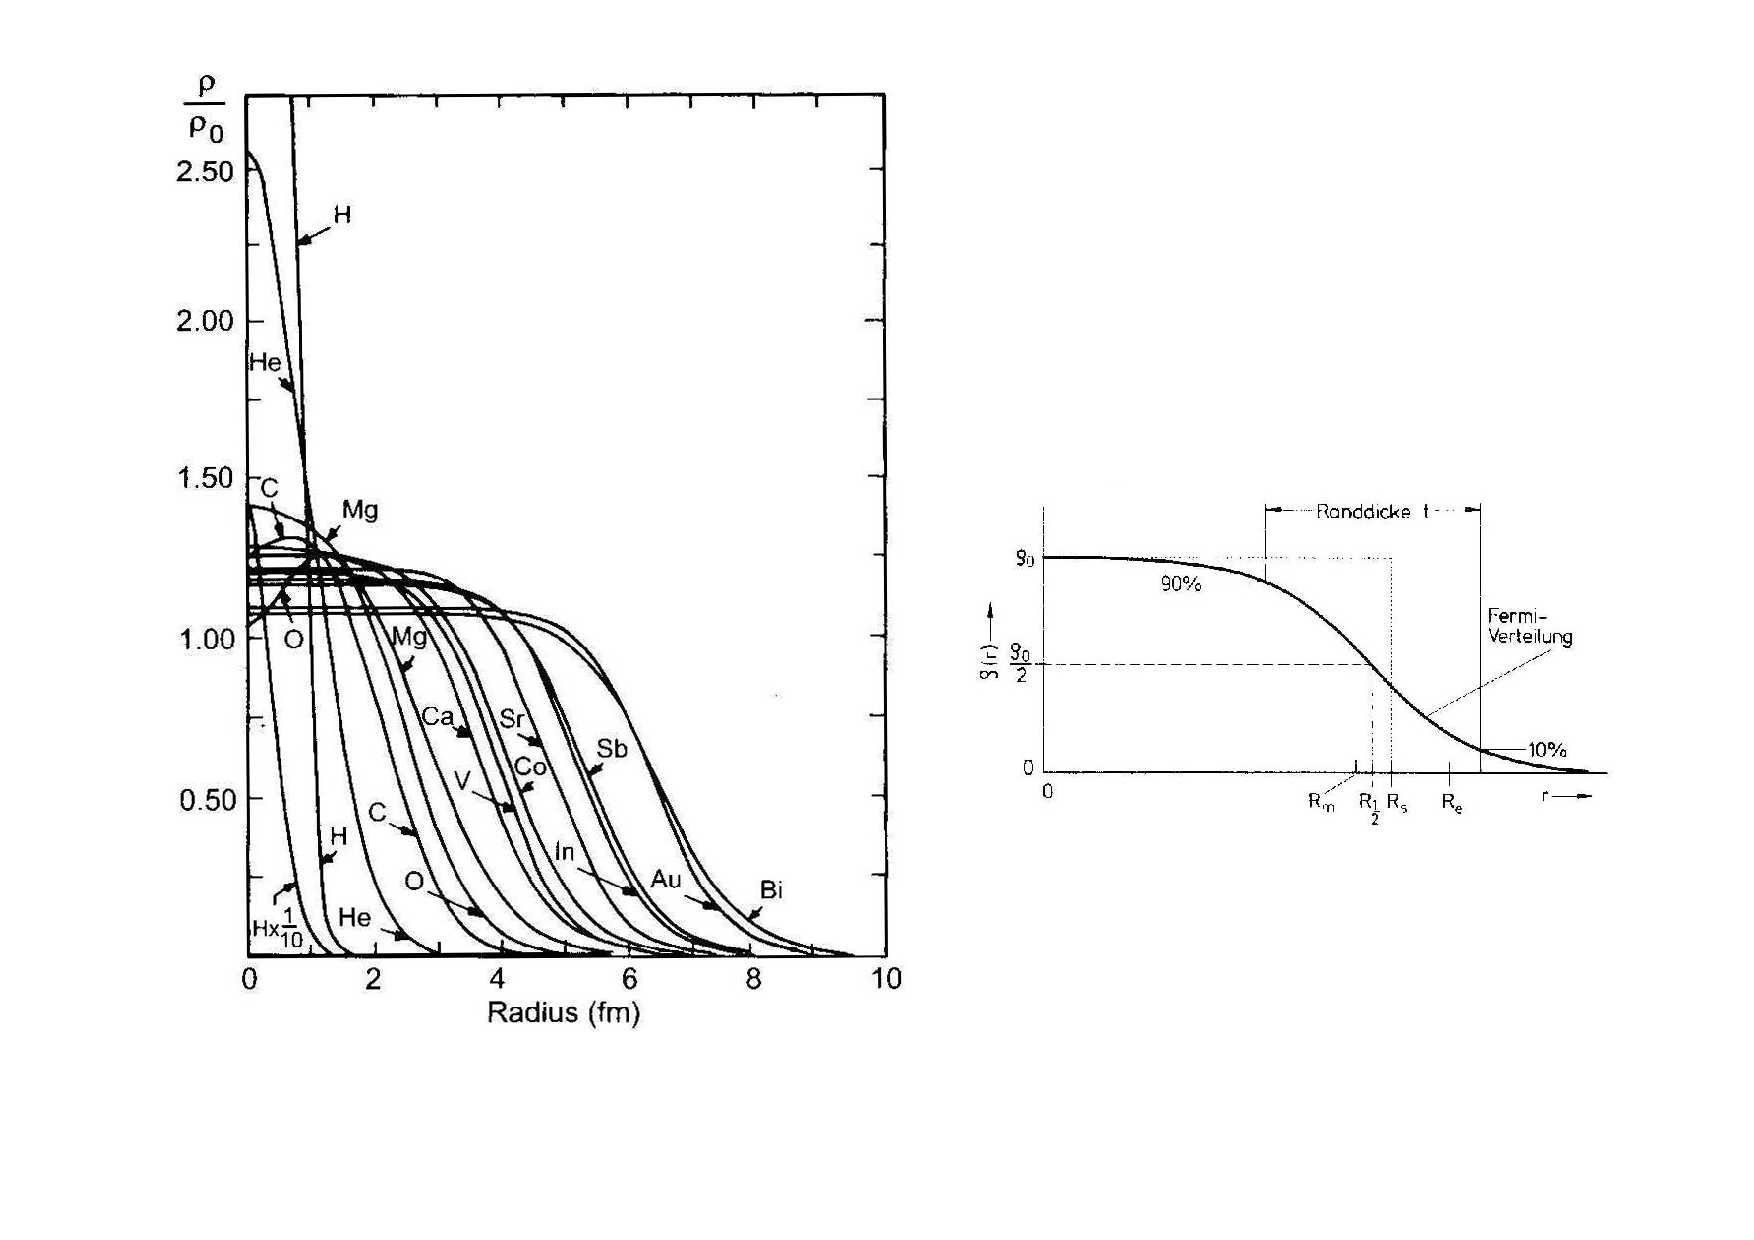
\includegraphics[width=\textwidth]{fig/2-StreuungLadungsvert.pdf}
% \end{figure}
\end{enumerate}
\end{bspn}
\begin{bemn}
Streuversuche kann man als Mikroskopie mit Materiewellen verstehen. Es gelten
die selben Auflösungsgesetze wie in der optischen Mikroskopie, d.h. die
Auflösung $\entspr$ Wellenlänge, wobei hier die De-Broglie Wellenlänge
\begin{align*}
\lambda_{dB} = \frac{h}{p},
\end{align*}
mit dem relativistischen Impuls $p$ gemeint ist. Für eine vorgegebene
$E_\text{kin}$ erhalten wir aus dem $p$-Skalarprodukt,
\begin{align*}
&E^2 = p^2c^2 +m_e^2c^4 = (E_\text{kin}+m_ec^2)^2.\\
\Rightarrow & p = \frac{1}{c}\sqrt{(E_\text{kin}+m_ec^2)^2 - m_e^2c^4}
= \frac{1}{c}\sqrt{E_\text{kin}^2+2E_\text{kin}m_ec^2+m_e^2c^4 - m_e^2c^4}
\\ &= \frac{1}{c}\sqrt{E_\text{kin}(E_\text{kin}+2m_ec^2)},\\
\Rightarrow & \lambda_{dB} =
\frac{hc}{\sqrt{E_\text{kin}}\sqrt{E_\text{kin}+2m_ec^2}}.
\end{align*}
Für $E_\text{kin}=100 \mathrm{MeV}$ ergibt sich $\lambda_{dB}\approx
10^{-14}\mathrm{m} = 10 \mathrm{fm}$, was noch zu wenig für Kernauflösung ist.
Bei der Verwendung von Elektronen werden aufgrund der geringen Masse für
Kernauflösung sehr hohe Energien benötigt. Während bei $\alpha$-Teilchen
bereits eine Energie von $5 \mathrm{MeV}$ ausreicht, sind bei Elektronen $500
\mathrm{MeV}$ notwendig.\maphere
\end{bemn}

\sfigure[H][0.6]%
	{2-WirkungsquerschnittUndLadungsverteilung.pdf}%
	{\FrauenfelderHenley, S. 163}
	{Wirkungsquerschnitt und Ladungsverteilung. Das Beugungsminimum im
	Wirkungsquerschnitt der schweren Kerne weist auf die wohldefinierte
	Kernoberfläche hin. Nukleonen dagegen besitzen eine langsam abnehmende
	Ladungsdichte an der Oberfläche.}

\subsection{Inelastische Streuung, Quarks und QCD}
Geht man zu Streuteilchen mit noch höherer Energie über und betrachtet die
verbleibenden Energie der gestreuten Teilchen, kann man Aufschluss über die
innere Struktur der Kerne und Nukleonen erhalten. Wir betrachten dazu die
Energie der gestreuten Teilchen als Funktion der Energie.
 
Bei Protonen kann man so feststellen, dass innere Anregungszustände existieren
(vgl. Spektrallinien) und diese daher eine innere Struktur besitzen, also aus
kleineren Teilchen aufgebaut sind.

\begin{figure}[!htpb]
\centering
\begin{minipage}{1\linewidth}%
	\renewcommand{\footnoterule}{}%
	\centering%
	\begin{pspicture}(0,-3)(11,5)
	\rput(5,0){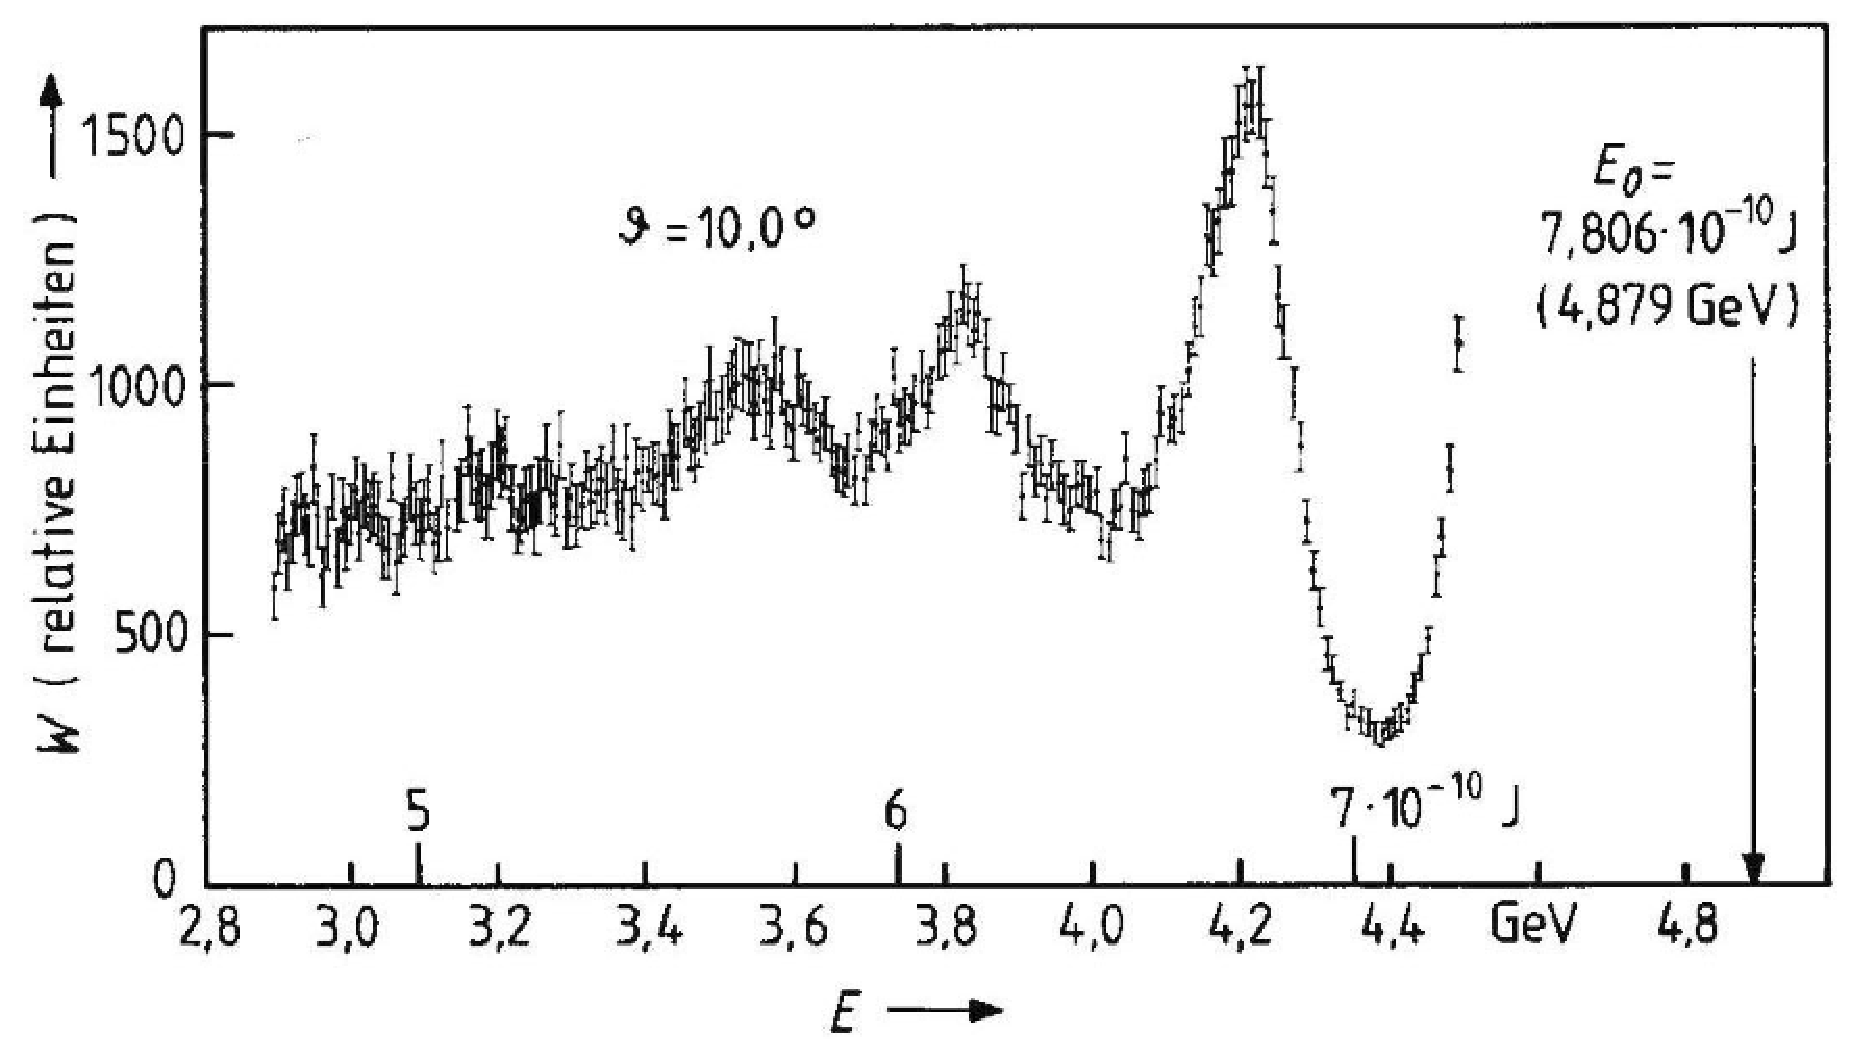
\includegraphics[width=10cm]{fig/2-InelastProton.eps}}
	\psline[linecolor=darkblue]{<-}(6.8,3)(6.8,4.2)
	\psline[linecolor=darkblue]{<-}(9.45,3)(9.45,4.2)
	\psline{<->}(7,3.6)(9.2,3.6)
	\rput(8.1,4){\color{gdarkgray}$\Delta E$}
	\rput(6.4,4.7){\color{gdarkgray}inelastischer Peak}
	\rput(9.6,4.7){\color{gdarkgray}elastischer Peak}
	\end{pspicture}
	\footnotetext{\textit{K. Stierstadt}, Physik der Materie, S. 28}
\end{minipage}
\caption{Nachweis der inneren Struktur von Protonen durch Streuung von
hochenergetischen Elektronen. Bei den inelastischen Peaks ist jeweils eine
Energie $\Delta E$ vom Target absorbiert worden, um in einen angeregten Zustand
überzugehen.}
\end{figure}

% \sfigure[!htpb]%
% 	{2-InelastProton.pdf}%
% 	{\textit{K. Stierstadt}, Physik der Materie, S. 28}
% 	{Nachweis der inneren Struktur von Protonen durch Streuung von
% 	hochenergetischen Elektronen.}

Für bestimmte Energien der streuenden Teilchen tritt Resonanz auf, d.h. im
Proton werden Energieniveaus mit dieser bestimmten Energie angeregt. 
Übersetzten wir das Energiemuster in ein Anregungsschema, sehen wir, dass
$p^+$ und $n^0$ dieselben Anregungsspektren besitzen. Ein analoges Ergebnis
erhalten wir für $\Delta$-Teilchen. \begin{figure}[!htbp]
	\centering
	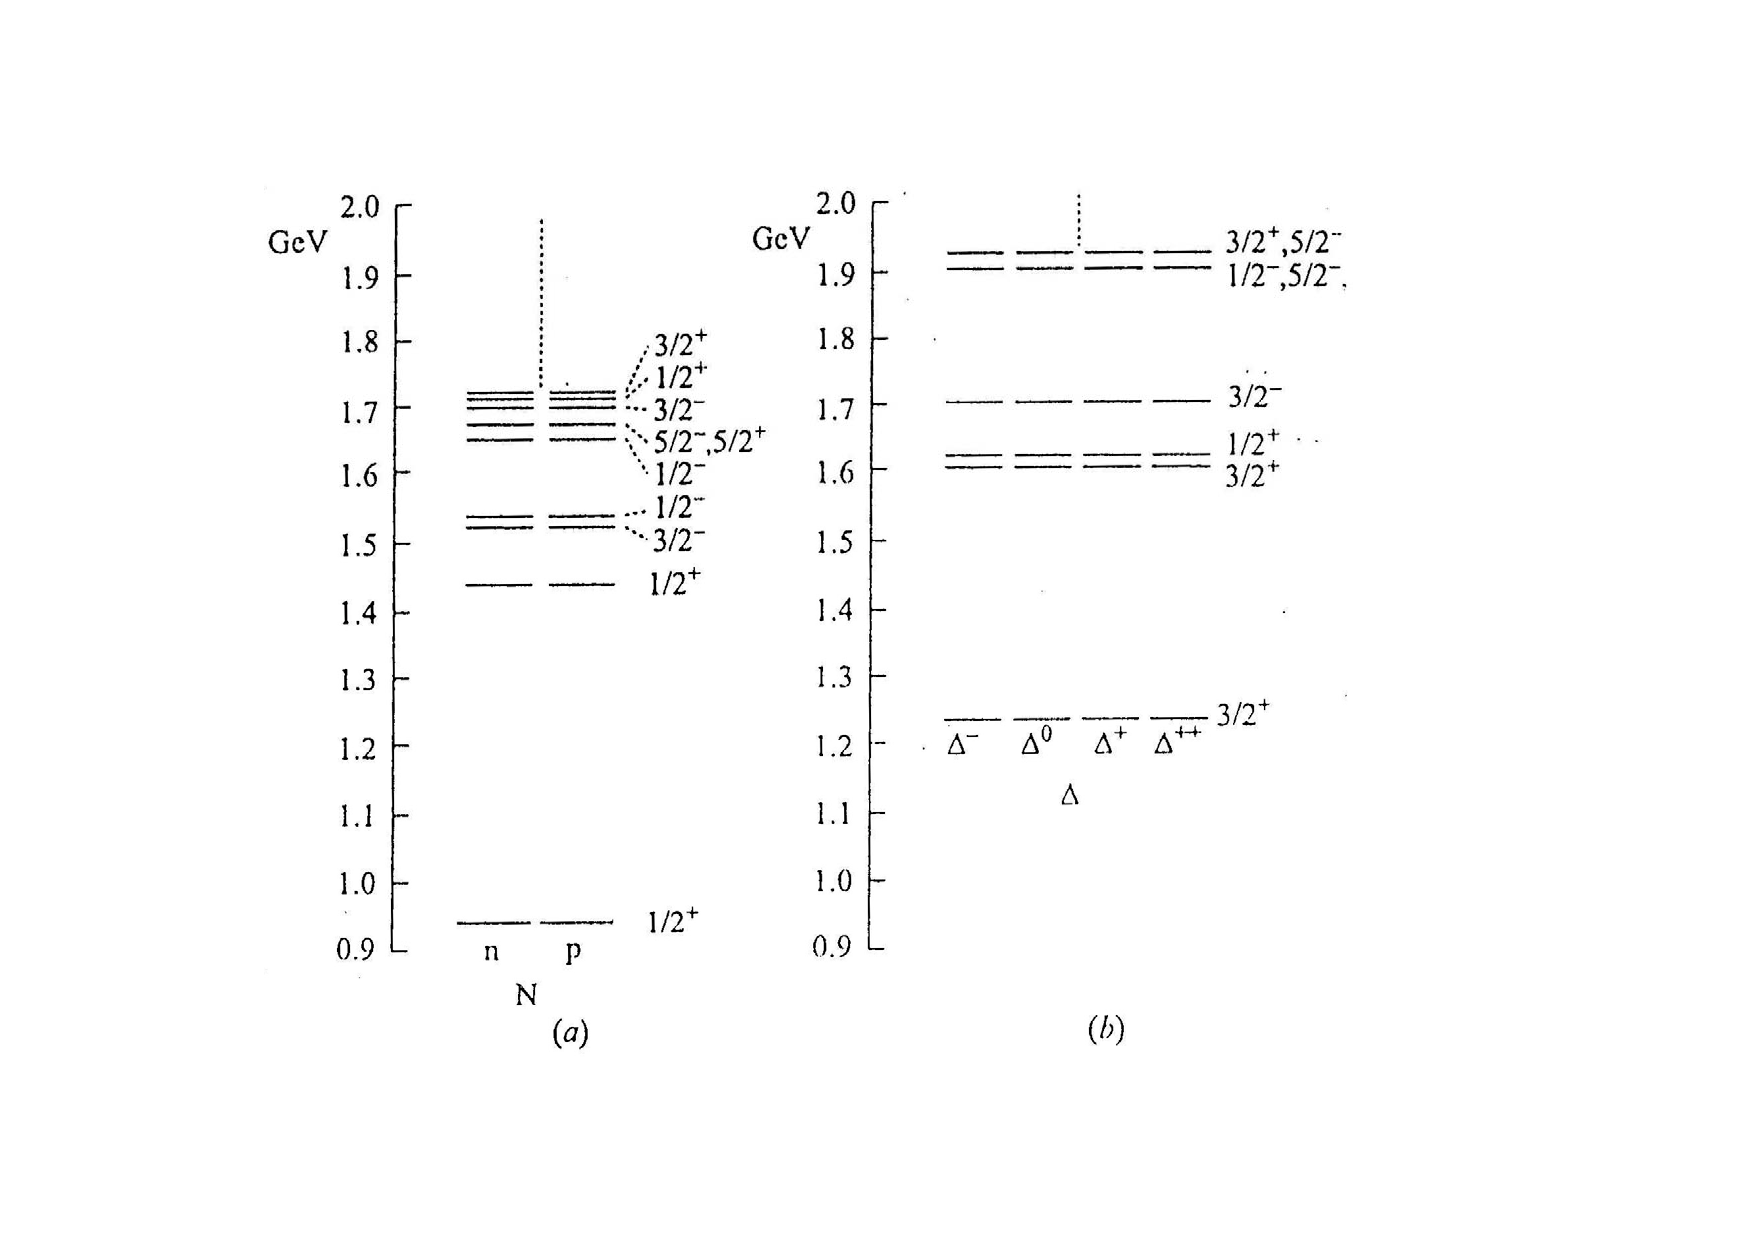
\includegraphics[width=0.8\textwidth]{fig/2-AnregungBaryonen.pdf}
	\caption{Anregungszustände Baryonen. (a) Doublett (N), (b) Quartett
	($\Delta$).}
\end{figure}

Wir haben bereits gesehen, dass es zu jedem Spin $s$, $2s+1$ entartete Zustände
gibt. Für Spin $s=\frac{1}{2}$ gibt es somit zwei Zustände $p^+,n^0$, für
$s=\frac{3}{2}$ vier Zustände, $\Delta^-, \Delta^0, \Delta^+, \Delta^{++}$. Da
für diese Teilchen innere Anregungszustände existieren, können sie nicht
elementar sein und müssen daher aus weiteren Teilchen bestehen,
den \emph{Quarks}.


Quarks müssen als elementare Teilchen, den kleinstmöglichen positiven Spin
$s=\frac{1}{2}$ besitzen.
Angenommen, die uns bekannten Baryonen bestünden nur aus zwei Quarks mit Spin
$s=\frac{1}{2}$, dann wären bei Kopplung von zweien nur Spinwerte von $s=0$
oder $1$ möglich, was nicht unserer Beobachtung entspricht. Die Baryonen müssen
daher aus mindestens drei Quarks bestehen.
Eine geradzahlige größere Anzahl von Quarks wäre
aufgrund der daraus resultierenden geradzaligen Spinwerten nicht möglich.
Eine
größere ungerade Anzahl wie z.b. $5$ wäre möglich, dann müssten
wir aber auch Baryonen mit entsprechendem Spin beobachten, was (noch) nicht der
Fall ist.

Gehen wir also davon aus, dass ein Baryon aus drei Quarks besteht. 
Quarks sind Fermionen, es kann von jeder Sorte nur ein Vertreter
pro Baryon koppeln (Pauli Prinzip). Es muss also mindestens $3$ verschiedene
Quarksorten geben, die für die innere Struktur verantwortlich sind. 

Auffällig ist, dass mehr positiv als negativ geladene Baryonen ($p^+$,
$\Delta^{++}$, $\Delta^+$) existieren, daher ist es wahrscheinlich, dass
mindestens eine Quarksorte eine große positive Ladung besitzt.

Wir wollen nun die Freiheitsgrade der Quarks genauer betrachten. Zunächst 
gibt es zwei Einstellungsmöglichkeiten für die Ladung, nämlich up mit der
Ladung $+\frac{2}{3}$ und down mit der Ladung $-\frac{1}{3}$, weshalb wir von
\emph{Up-} und \emph{Downquarks} sprechen. Diese Einstellungsmöglichkeiten
sind jedoch vom Spin der Quarks selbst unabhängig, ein Upquark hat daher auch
2 Spineinstellungsmöglichkeiten, Spin up und down. Die uns bekannten Baryonen
haben somit die Konfiguration,
\begin{align*}
&n^0 = (u^{\uparrow+\frac{2}{3}},
 	  d^{\uparrow-\frac{1}{3}}, 
	  d^{\downarrow-\frac{1}{3}})\\
&p^+ = (u^{\uparrow+\frac{2}{3}},
 	  u^{\uparrow+\frac{2}{3}}, 
	  d^{\downarrow-\frac{1}{3}})\\
&\Delta^- = (d^{\uparrow-\frac{1}{3}},
 	  d^{\uparrow-\frac{1}{3}},
 	  d^{\uparrow-\frac{1}{3}})\\
&\Delta^0 = (u^{\uparrow+\frac{2}{3}},
 	  d^{\uparrow-\frac{1}{3}},
 	  d^{\uparrow-\frac{1}{3}})\\
&\Delta^+ = (u^{\uparrow+\frac{2}{3}},
 	  u^{\uparrow+\frac{2}{3}},
 	  d^{\uparrow-\frac{1}{3}})\\
&\Delta^{++} = (u^{\uparrow+\frac{2}{3}},
 	  u^{\uparrow+\frac{2}{3}},
 	  u^{\uparrow+\frac{2}{3}}).
\end{align*}
Wir sehen, dass die Teilchenkonfigurationen ohne weitere Freiheitsgrade
nicht möglich sind, da sich maximal zwei Quarks des selben Typs durch ihre
Spineinstellung unterscheiden können. Beim $\Delta^{++}$-Teilchen haben wir
jedoch drei Teilchen des selben Typs, was nach dem Pauli Prinzip verboten wäre.

Es muss also weitere Freiheitsgrade geben und zwar mindestens drei. Wir nennen
diese \emph{Farbladung (color charge)}  $(r,g,b)$ für rot, grün und blau. Die
Farbladung ist die Ladung der starken Wechselwirkung und wird in der
Quantenchromodynamik genauer betrachtet. Wir wollen hier lediglich eine
qualitative Betrachtung durchführen.

\begin{figure}[H]
\centering
\begin{pspicture}(0,-1.47)(3.46,1.47)
\pscircle[linecolor=red](1.69,-1.14){0.33}
\pscircle[linecolor=green](3.13,0.74){0.33}
\pscircle[linecolor=blue](0.33,0.74){0.33}
\pscircle[linecolor=htmlyellow](1.69,1.14){0.33}
\pscircle[linecolor=cyan](3.11,-0.64){0.33}
\pscircle[linecolor=magenta](0.33,-0.64){0.33}
\rput(0.34,0.75){$r$}
\rput(3.13,0.75){$g$}
\rput(1.7,-1.12){$b$}

\rput(3.13,-0.61){$\overline{r}$}
\rput(0.33,-0.61){$\overline{g}$}
\rput(1.7,1.2){$\overline{b}$}
\psline[linewidth=0.04cm](0.54,-0.35)(1.46,0.87)
\psline[linewidth=0.04cm](1.92,0.87)(2.92,-0.33)
\psline[linewidth=0.04cm](0.68,-0.63)(2.76,-0.63)
\psline[linewidth=0.04cm,linestyle=dashed,dash=0.16cm 0.16cm](0.68,0.71)(2.78,0.71)
\psline[linewidth=0.04cm,linestyle=dashed,dash=0.16cm 0.16cm](0.52,0.45)(1.5,-0.85)
\psline[linewidth=0.04cm,linestyle=dashed,dash=0.16cm 0.16cm](1.88,-0.85)(2.92,0.47)
\end{pspicture}
\caption{Farbladungen und Antifarbladungen.}
\end{figure}

In der Elektrostatik kann man die Ladungskonjugation als Punktspiegelung
auffassen. Bei den Farbladungen existiert z.B. für rot ein
\oline{rot}, das Gegenteil von rot, es entspricht aber weder grün
oder blau. Für die Ladungskonjugation gilt daher,
\begin{align*}
\begin{pmatrix}
r \\ g \\ b
\end{pmatrix}
\overset{\hat{C}}{\mapsto}
\begin{pmatrix}
\overline{r} \\ \overline{g} \\ \overline{b}
\end{pmatrix}.
\end{align*}
Die für uns beobachtbaren Teilchen (Baryonen) sind jedoch farblos, d.h.
Baryonen eines Typs sind nicht unterscheidbar und wechselwirken nicht direkt
(d.h. in 1. Ordnung) durch den Mechanismus der Quarkwechselwirkungen.
\begin{bspn} Mögliche Konfiguration eines $\Delta^{++}$,
\begin{align*}
\Delta^{++} = (u^{\uparrow+\frac{2}{3}g},
 	  u^{\uparrow+\frac{2}{3}r},
 	  u^{\uparrow+\frac{2}{3}b})\bsphere
\end{align*}
\end{bspn}
\begin{bspn}
Es ist aber auch möglich, ein rot und ein \oline{rot} zusammenzubringen,
wodurch ein fabloses Teilchen, ein \emph{Meson} entsteht.
\begin{align*}
\pi^0 = (u^{r}\overline{u}^{\overline{r}}).
\end{align*}
Mesonen bestehen aus zwei Quarks. Aufgrund der Ladungen sind somit auch
Triplets möglich. Da Mesonen aus Quarks und Antiquarks bestehen haben sie eine
sehr endliche Lebensdauer ($\pi^0$ von $2.6\cdot 10^{-8}s$).\bsphere
\end{bspn}

Die Farbladungen führen zu Wechselwirkungen zwischen den Quarks. Wir können
diese Wechselwirkung durch das Modelpotential,
\begin{align*}
V(r) = -\frac{\alpha_s}{r} + Ar
\end{align*}
beschreiben.

Im Gegensatz zum Coulomb-Potential bei dem ein Teilchen durch das Aufbringen
von endlich viel Energie unendlich weit vom Potentialmittelpunkt entfernt
werden kann, nimmt hier das Potential mit wachsendem Abstand linear zu.
Beim Versuch Farbladungen zu trennen, entstehen neue farblose Mesonen, wenn die
Wechselwirkungsenergie größer wird als die Ruhemasse des Mesons.

\sfigure[!htpb]%
	{2-MesonenTrennung.pdf}%
	{\KuckukKern, S. 188}%
	{Zum Blasenmodell der Hadronen (Bag Modell).}

Insgesamt ist so weniger Energie notwendig als für die Trennung der einzelnen
Farbladungen. Als Konsequenz sehen wir, dass es nur farblose Teilchen als
beobachtbare Teilchen auftreten.

Es handelt sich hier lediglich um eine stark vereinfachte Modellvorstellung,
die schnell an ihre Grenzen stößt. In Wirklichkeit ist die Wechselwirkung
deutlich komplizierter, eine detailierte Behandlung ist aber für unsere
Fragestellung nicht zweckmäßig und sprengt den Rahmen der Vorlesung.

Wir wollen nun zur Kernphysik zurückkehren und die Frage klären, warum auch
farblose Teilchen wie $p^+, n^0$ eine attraktive Wechselwirkung erfahren.
Aufgrund der Ladung lässt sich eine Coulomb-Wechselwirkung sofort ausschließen.
Erinnern wir uns zunächst an die Van-Der-Waals Wechselwirkung. Hier induzieren
Atome durch fluktuierende Ladungsverschiebung in anderen Atomen Dipolmomente,
wodurch eine Attraktion zwischen den Atomen stattfindet. Ähnlich induzieren
auch fluktuierende Farbladungsverschiebungen, Farbladungsverschiebungen in
anderen Teilchen, wodurch diese ebenfalls eine attraktive Wechselwirkung
erfahren. Diese Wechselwirkung ist als Induktionsprozess 2. Ordnung 
schwächer als die Wechselwirkung zwischen den Farbladungen selbst; bei
den im Atom vorliegenden Längenskalen jedoch deutlich stärker als beispielsweise
die Coulomb Wechselwirkung für gleichnamige Teilchen.

Wir wollen diese Wechselwirkung nun für den konkreten Fall der
Proton-Neutron-Wechselwirkung betrachten. Durch den Induktionsprozess werden
hier $\pi^+$-Mesonen, farblose Teilchen, die aus einem Up-Quark
und einem Anti-Down-Quark bestehen, ausgetauscht.
 \begin{figure}[!htbp]
\centering
\begin{pspicture}(0,-0.8)(3.76,1)
\pscircle(0.59,-0.2028125){0.59}
\pscircle(3.17,-0.2028125){0.59}

\rput[b](0.32953125,-0.1){\color{gdarkgray}u}
\rput[b](0.8095313,-0.1){\color{gdarkgray}u}
\rput(0.56453127,-0.5){\color{gdarkgray}d}

\rput[b](2.9095314,-0.1){\color{gdarkgray}u}
\rput[b](3.3845313,-0.1){\color{gdarkgray}d}
\rput[b](3.1445312,-0.5){\color{gdarkgray}d}

\psline[linecolor=darkblue]{<->}(1.22,-0.1528125)(2.52,-0.1528125)

\rput(0.6045312,0.7371875){\color{gdarkgray}$p^+$}
\rput(3.188125,0.7371875){\color{gdarkgray}$n^0$}
\rput(1.9445312,0.2171875){\color{gdarkgray}$\pi^+$}
\end{pspicture} 
\qquad
\begin{pspicture}(0,-2.2)(3.26,2.3)
\psellipse(0.42,0.995625)(0.4,0.78)

\psellipse(2.86,0.995625)(0.4,0.78)

\psellipse(0.4,-0.984375)(0.4,0.78)


\psellipse(2.86,-0.984375)(0.4,0.78)

\psline(0.9,1.515625)(2.4,1.515625)
\psline(0.92,1.015625)(2.4,1.015625)
\psline(0.92,-0.964375)(2.4,-0.964375)
\psline(0.92,-1.364375)(2.4,-1.364375)

\psline[linecolor=yellow]{->}(2.4,0.575625)(1.94,0.575625)(1.36,-0.5)(0.92,-0.5)
\psline[linecolor=darkblue]{->}(0.92,0.595625)(1.38,0.595625)(1.96,-0.5)(2.4,-0.5)

\psellipse(1.65,0.075625)(0.55,0.3)


\rput[b](0.4,1.4){\color{gdarkgray}d}
\rput[b](0.4,0.95){\color{gdarkgray}u}
\rput[b](0.4,0.5){\color{gdarkgray}u}

\rput[b](2.85,1.4){\color{gdarkgray}d}
\rput[b](2.85,0.95){\color{gdarkgray}u}
\rput[b](2.85,0.5){\color{gdarkgray}d}

\rput[b](0.4,-0.6){\color{gdarkgray}d}
\rput[b](0.4,-1.05){\color{gdarkgray}u}
\rput[b](0.4,-1.5){\color{gdarkgray}d}

\rput[b](2.85,-0.6){\color{gdarkgray}u}
\rput[b](2.85,-1.05){\color{gdarkgray}u}
\rput[b](2.85,-1.5){\color{gdarkgray}d}

\rput[b](1.9695313,-0.05){\color{gdarkgray}u}
\rput[b](1.3445313,-0.05){\color{gdarkgray}\oline{d}}

\rput[b](0.4,2){\color{gdarkgray}$p^+$}

\rput[b](2.85,2){\color{gdarkgray}$n^0$}

\rput[b](0.4,-2.1){\color{gdarkgray}$n^0$}

\rput[b](2.85,-2.1){\color{gdarkgray}$p^+$}
\end{pspicture} 
\caption{Rolle des $\pi^+$-Meson bei der Proton-Neutron Wechselwirkung.}
\end{figure}

Um diese Wechselwirkung mit anderen uns bekannten zu vergleichen, müssen wir
die Wechselwirkungteilchen vergleichen. Die Elektromagnetische Wechselwirkung
basiert beispielsweise auf Photonen, die keine Ruhemasse und daher unendliche
Reichweite haben. Die Mesonen dagegen besitzen eine Ruhemasse und haben daher
nur eine endliche Reichweite. Mithilfe der Energie-Masse-Äquivalenz und der
Heisenbergschen Unschärferelation können wir die Reichweite abschätzen. Gehen wir von
\begin{align*}
\Delta t = \frac{\hbar}{\Delta E}
\end{align*} 
aus, wobei $\Delta E \ge m_{\pi}c^2$, so erhalten wir für die Reichweite,
\begin{align*}
R = c\Delta t = \frac{c\hbar}{\Delta E} \le \frac{\hbar}{cm_\pi}.
\end{align*}
Für $\pi$-Mesonen mit $m_\pi = 140 \frac{\mathrm{MeV}}{c^2}$ ergibt sich der
Wert,
\begin{align*}
R \le 1.4\mathrm{fm}.
\end{align*}
 \begin{figure}[!htbp]
\centering
\begin{pspicture}(0,-1.3425)(4.8096876,1.3225)

\psbezier[linecolor=darkblue](0.5046875,-0.9175)(1.1446875,-0.2175)(1.1046875,0.6825)(0.6468304,1.3025)
\psbezier[linecolor=yellow](3.8646874,-0.9175)(3.2246876,-0.2175)(3.2646875,0.6825)(3.7225447,1.3025)

\pscircle[fillstyle=solid,fillcolor=glightgray](0.7746875,-0.5275){0.19}
\pscircle[fillstyle=solid,fillcolor=glightgray](3.4746876,-0.3075){0.19}
\psline(0.6646875,1.0425)(0.8846875,1.1825)
\psline(0.8446875,0.3025)(1.1246876,0.3025)

\psline[linestyle=dotted,dotsep=0.06cm]{->}(1.1046875,0.3625)(3.3846874,0.9425)
\psdots(3.5246875,0.9625)

\rput(0.735,-1.1875){\color{gdarkgray}Nukleon 1}
\rput(4.0295315,-1.1875){\color{gdarkgray}Nukleon 2}
\rput(0.5565625,0.6725){\color{gdarkgray}$\Delta x$}
\rput(2.2190626,0.3925){\color{gdarkgray}$\Delta t$}
\end{pspicture} 
\caption{Reichweite der Wechselwirkung.}
\end{figure}

Aufgrund unserer stark vereinfachten Modellvorstellung ist dieses Vorgehen nur
ein zur groben Abschätzung der Reichweite zulässiges Mittel.

Wir sehen also, dass die 2. Ordnung Farbwechselwirkung, die durch den Austausch
von $\pi$-Mesonen stattfindet, eine Reichweite von ungefähr Kerndurchmesser
hat. Die Teilchen im Kern wechselwirken also hauptsächlich untereinander. Damit
sie mit Teilchen in anderen Kernen
wechselwirken, müsste man die Kerne auf einen Abstand kleiner als der
Kerndurchmesser zusammenbringen.\footnote{Dies ist eine große Herausforderung
beim Bau von Fusionsreaktoren.}

\sfigure[htpb][1]%
	{2-TheQuarks.pdf}%
	{\TiplerMPFife, S. 569}%
	{Quarks.}
	
\sfigure[htpb][1]%
	{2-TheLeptons.pdf}%
	{\TiplerMPFife, S. 569}%
	{Leptonen.}

\subsection{Kernmassenbestimmung und Kernmodelle} 

Wir wollen nun die Bindungsenergie der 2. Ordnung Farbladungswechselwirkung
untersuchen. Es stellt sich natürlich die Frage, wie man diese überhaupt messen
kann. Die Energie Masse Äquivalenz $E=mc^2$ besagt, dass die Information über
die  Bindungsenergie bereits in der Masse enthalten ist. Eine Änderung der
Bindungsenergie führt somit zu einer Änderung der Masse. Misst man nun die
Masse der einzelnen Nukleonen und anschließend die der Atome, kann man aus der
Differenz der Massen die Größe der Bindungsenergien berechnen.

\begin{figure}[!htbp]
	\centering
	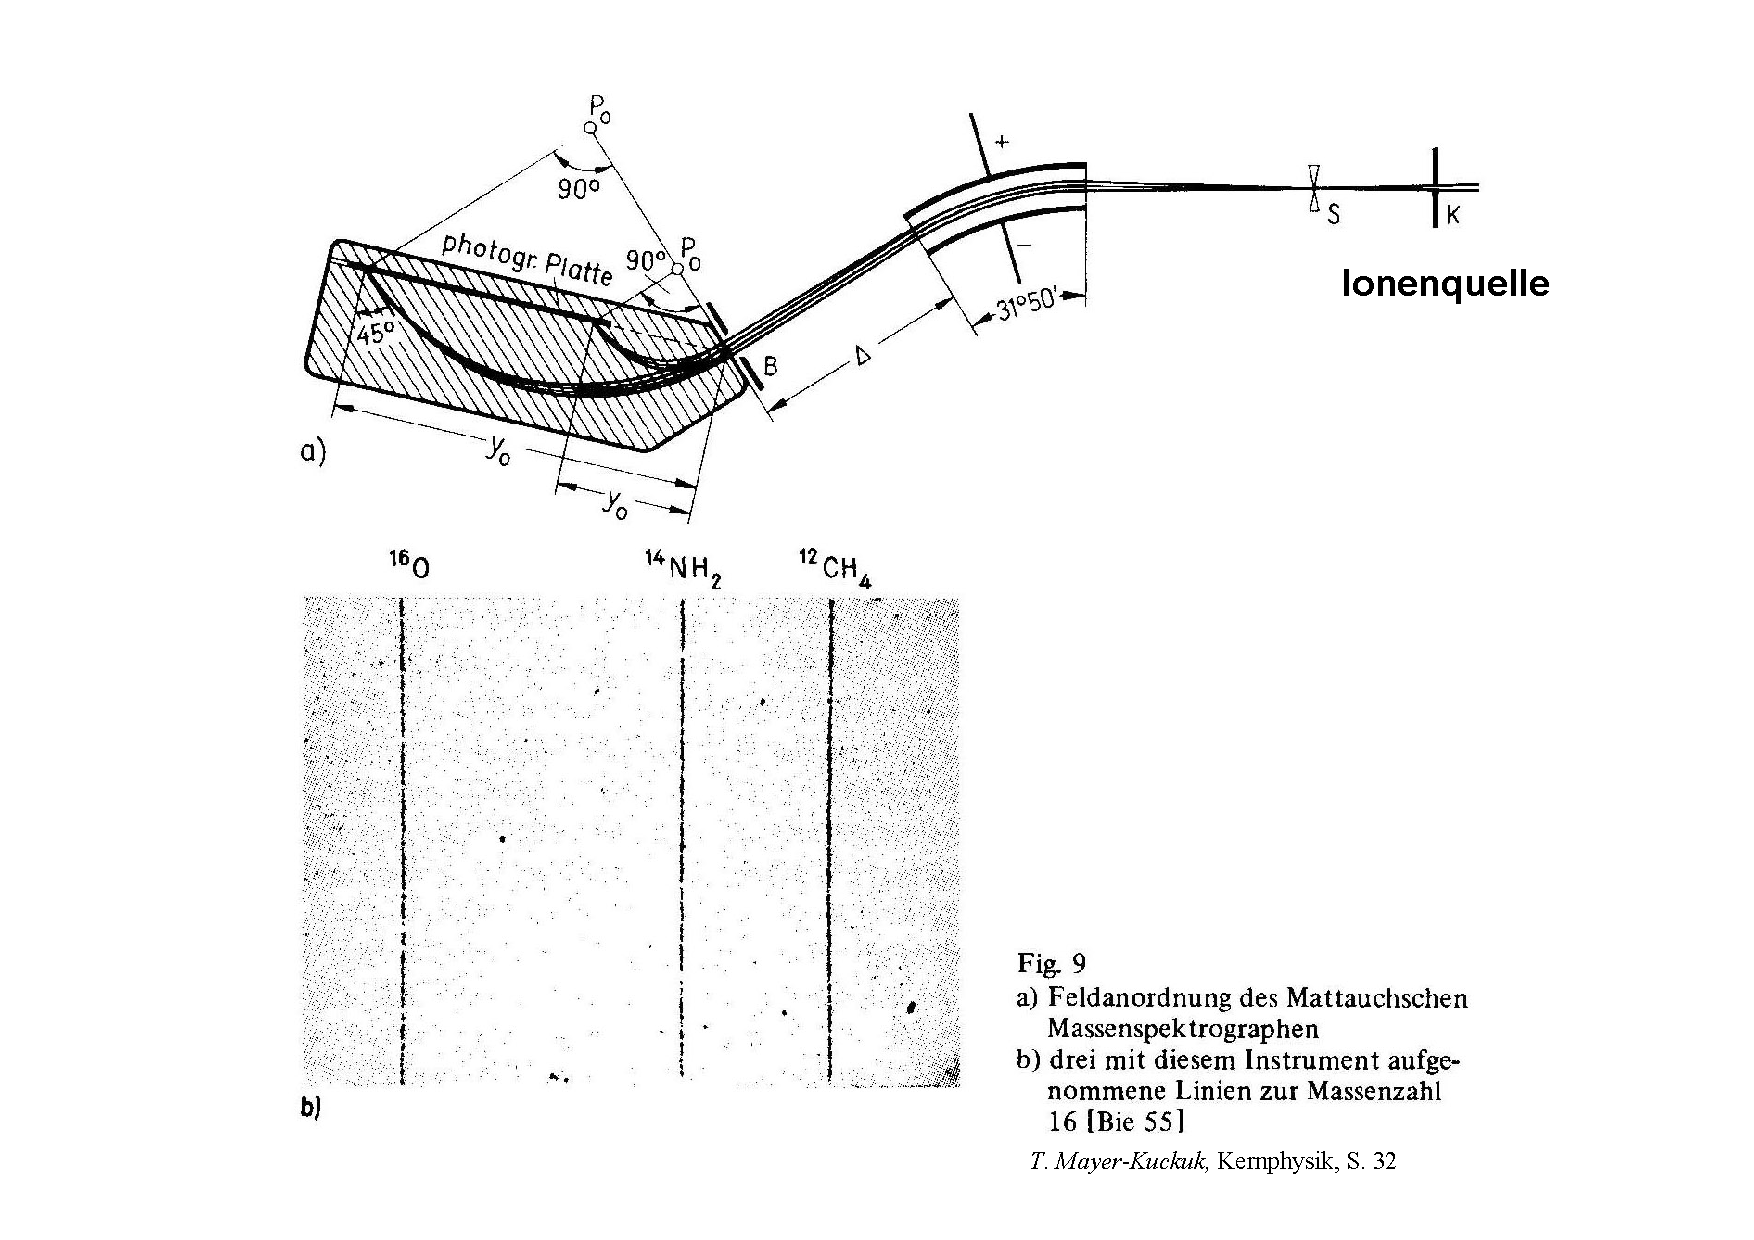
\includegraphics[width=0.8\textwidth]{fig/2-Massenspektrograph.pdf}
\end{figure}

\begin{defnn}
Die \emph{Bindungsenergie} ist eine positive Größe, gegeben durch
\begin{align*}
B(Z,N) = \left[Zm_{p^+} + Nm_{n^0} - m(Z,N) \right]c^2,
\end{align*}
wobei $Z$ die Anzahl der Protonen, $N$ die Anzahl der Neutronen und $m(Z,N)$
die reale Masse eines Kerns mit $N$ und $Z$ bezeichnet.\fishhere
\end{defnn}
\begin{bspn} Masse des
Protons, Neutrons und Elektrons
\begin{align*}
m_{p^+} = 938.3\frac{\mathrm{MeV}}{c^2},\quad m_{n^0} =
939.6\frac{\mathrm{MeV}}{c^2},\quad m_{e^-} = 0.591\frac{\mathrm{MeV}}{c^2}.
\end{align*}
Die Elektronenmasse ist also vernachlässigbar gegenüber der der
Protonen und Neutronen.\bsphere
\end{bspn}
\begin{bspn}
Die Atomare Masseneinheit
\begin{align*}
1u = \frac{1}{12}m\left({}^{12}C\right) = 931.5\frac{\mathrm{MeV}}{c^2} \entspr
1.6606\cdot 10^{-24}\mathrm{g},
\end{align*}
ist kleiner als die Summe der einzelnen Protonen- und Neutronenmassen im
${}^{12}C$, es fehlt also bereits die ${}^{12}C$-Bindungsenergie.\bsphere
\end{bspn}
\begin{bspn}
Die Messgenauigkeit der Massenspektrometrie heute $\dfrac{\Delta m}{m} \approx
10^{-10}$.\bsphere
\end{bspn}

\sfigure%
	{2-BindungsEnergieProNukleon.pdf}
	{\KuckukKern, S. 36}
	{Zentrales Ergebnis der Massenspektroskopie: Bindungsenergie pro Nukleon als
	Funktion von $A$ für stabile Kerne.}

Wollen wir Atome vergleichen, benötigen wir noch einige Begriffe. 

\begin{figure}[!ht]
  \centering
  \begin{pspicture}(-2.6,-1.2)(5,1.2)

\psbezier{->}(2.9721875,0.7107813)(2.4521875,-0.08921875)(2.4321876,1.0707812)(1.8121876,0.41078126)
\psbezier{<-}(1.9574513,0.014663258)(2.5974512,-0.44533673)(1.8574514,-0.68533677)(2.4574516,-0.9253368)
\psbezier{->}(0.3121875,0.45078126)(0.8321875,-0.12921876)(0.8521875,1.0307813)(1.3321875,0.45078126)
\psbezier{<-}(1.2471875,0.008774293)(0.4871875,0.008774293)(1.0671875,-0.6712257)(0.4071875,-0.5712257)

\rput(1.6289062,0.20578125){\color{darkblue}\Large ${}_Z^AX_N$}

\rput[l](2,0.9607813){\color{gdarkgray}chemisches Element}
\rput[l](2.6,-0.9792187){\color{gdarkgray}Neutronenzahl}
\rput[r](0.7,0.6407812){\color{gdarkgray}Gesamtnukleonenzahl}

\rput[r](0.6,-0.3){\color{gdarkgray}Kernladungszahl}
\end{pspicture} 
  \caption{Notation eines chemischen Elements $X$ mit Kernladungszahl $Z$,
  Neutronenzahl $N$ und Gesamtnukleonenzahl $A$.}
\end{figure}

\begin{defnn}
\emph{Isotope} sind Kerne mit gleicher Kernladungszahl $Z$ aber
unterschiedlicher Neutronenzahl $N$ und demnach unterschiedlicher Massenzahlen $A$.
\begin{bspn}
${}^{12}C$, ${}^{13}C$ und ${}^{14}C$.\bsphere
\end{bspn}
\emph{Isobare} sind Kerne mit derselben Massenzahl $A$, jedoch mit
unterschiedlicher Neutronenzahl $N$ und deshalb auch unterschiedlicher Kernladungszahl $Z$.
\begin{bspn}
${}^{12}C$, ${}^{12}N$ und ${}^{12}B$.\bsphere
\end{bspn}
\emph{Isotone} sind Kerne mit derselben Neutronenzahl $N$, aber mit
unterschiedlicher Massenzahl $A$ und deshalb auch unterschiedlicher
Kernladungszahl $Z$.
\begin{bspn}
${}^{12}C$, ${}^{13}N$ und ${}^{14}O$.\bsphere\fishhere
\end{bspn}
\end{defnn}

\begin{figure}[!htbp]
\centering
\begin{pspicture}(0,-1.2910937)(4.845,1.2910937)

\psline{->}(0.32,-1.1076914)(0.32,1.1726646)
\psline{->}(0.2753125,-1.07)(4.2353125,-1.07)
\psline[linecolor=darkblue](0.8553125,0.8726562)(3.6553125,-0.72734374)
\psline[linecolor=yellow](0.8553125,0.07320729)(3.6553125,0.07320729)
\psline(2.2553124,-0.72734374)(2.2553124,0.8726562)

\rput(2.325625,1.1226562){\color{gdarkgray}Isotone}

\rput(3.935625,0.36265624){\color{gdarkgray}Isotope}

\rput(4.275625,-0.75734377){\color{gdarkgray}Isobare}

\rput(4.405156,-1.1373438){\color{gdarkgray}$N$}

\rput(0.09796875,1.0826563){\color{gdarkgray}$Z$}
\end{pspicture} 
\caption{Isotone, Isotope und Isobare.}
\end{figure}

\begin{bemn}[Beobachtungen.]
\begin{enumerate}[label=\arabic{*}.)]
\item Die Bindungsenergie pro Nukelon $\frac{B}{A}$ hat ein Maximum bei $A\sim
60$. Wir können daher durch Spaltung von schweren bzw. Fusion von leichten
Kernen Energie gewinnen. Durch Fusion der leichtesten Kerne können über
$\approx 4\mathrm{MeV}$ frei werden, während wir durch Spaltung der schwersten
Kerne lediglich $\approx 1\mathrm{MeV}$ erhalten.
\item Leichte Kerne zeigen eine ``Schalenstruktur''.
\item Größenordnungsmäßig bleibt $\frac{B}{A}$ für schwere Kerne nahezu
konstant. Die Wechselwirkung eines Nukleons betrifft nur seine nächsten
Nachbarn, die weiteren Nukleonen im Kern spielen keine Rolle. Andernfalls würden
$A-1$ Bindungspartner auch $\frac{A(A-1)}{2}$ Bindungen erzeugen und $\frac{B}{A}$
wäre proportional zu $A$.
\end{enumerate}
\end{bemn}

Wir können diese Eigenschaften sehr gut mittels einem Tröpfchenmodell
beschreiben. In einem Tropfen herrscht unabhängig von der Größe des Tropfens
stets die selbe Dichte. Dies entspricht den Ergebnissen der Streuexperimente,
die eine nahezu homogene Ladungsverteilung für schwere Teilchen besagen. Ein
Teilchen in einem Tropfen wechselwirkt nur mit seinen nächsten Nachbarn. Die
Wechselwirkung ist von der Größe des Topfens unabhängig.

Das Tröpfchenmodell scheitert jedoch beim Übergang zu $<10$ Nukleonen und der
hier vorliegenden Schalenstruktur. In diesem Fall lassen sich die Teilchen als
nahezu ideales Gas interpretieren und durch das Modell des freien Teilchens
beschreiben.

Zur Lösung wählen wir als effektives Model ein Fermigas im
mittleren Potential. Innerhalb des Kastenpotentials kann sich ein Teilchen
frei bewegen, während am Rand viel Energie notwendig ist, um es vom Verband zu
lösen. Die Physik in diesem Potential wird durch das Pauli-Prinzip dominiert,
welches bestimmt wie oft ein Energiezustand überhaupt auftreten kann.

Wir werden sehen, dass die Energie dieses Potentials viel größer ist als die
Bindungsenergie pro Nukleon $E_\text{Fermi}>>\frac{B}{A}$.
\begin{bspn}
$E_\text{Fermi}\approx40\mathrm{MeV}$, $\dfrac{B}{A}\approx
8\mathrm{MeV}$.\bsphere
\end{bspn}
\begin{figure}[!ht]
  \centering
\begin{pspicture}(-0.25,-0.74717915)(2.42,0.7266349)

\psline(0,0.7066349)(0.7,0.7066349)(0.7,-0.6733651)(1.7,-0.6733651)(1.7,0.7066349)(2.4,0.7066349)
\psline(0.8,-0.32)(1.6,-0.32)
\psline(0.8,-0.023)(1.6,-0.023)
\psline[linecolor=darkblue](0.8,0.25)(1.6,0.25)

\pscircle[fillstyle=solid,fillcolor=white](0.91,0.25){0.09}
\pscircle[fillstyle=solid,fillcolor=white](0.91,-0.023){0.09}
\pscircle[fillstyle=solid,fillcolor=white](0.91,-0.32){0.09}

\pscircle[fillstyle=solid,fillcolor=white](1.49,0.25){0.09}
\pscircle[fillstyle=solid,fillcolor=white](1.49,-0.023){0.09}
\pscircle[fillstyle=solid,fillcolor=white](1.49,-0.323){0.09}

\rput[r](0.6,0.25663492){\color{gdarkgray}$E_\text{Fermi}$}
%\rput{90}(2.020937,1.8641888)
%{\rput(1.9125,-0.063365094){\color{gdarkgray}Zustände}}
\end{pspicture} 
  \caption{Kastenpotential mit diskreten Energiezuständen.}
\end{figure}

\subsubsection{Ideales Fermigas im Kastenpotential}

Die Wechselwirkung der Fermionen untereinander ist sehr klein im Verhältnis zur
Fermienergie, weshalb wir diese in unserem Modell vernachlässigen wollen.
Da Messungen außerdem zeigen, dass die Dichteverteilung nahezu konstant
ist, gehen wir davon aus, dass außer den elementaren keine weiteren Kräfte
wirken.

Wir wollen nun die quantenmechanischen Zustände im 3-dimensionalen
Kastenpotential untersuchen. Dazu wählen wir für die Nukleonen als effektives
Potential,
\begin{align*}
V(r) =
\begin{cases}
0 & r > a,\\
-V_0 & r\le a,
\end{cases}
\end{align*}
wobei $a$ den Kernradius bezeichnet.

Um unsere Rechnungen zu vereinfachen, gehen wir davon aus, dass der Kern
Würfelform mit Kantenlänge $a$ hat. Dadurch kommt in unserem
Modell lediglich ein Vorfaktor der Größenordnung $1$ dazukommt. Durch die
Würfelform können wir die 3-dimensionale Schrödingergleichung in drei
1-dimensionale separieren. Die Gesamtwellenfunktion ist somit gegeben durch,
\begin{align*}
\Psi_\text{ges} = \Psi_x\Psi_y\Psi_z,
\end{align*}
mit der Gesamtenergie,
\begin{align*}
E_\text{ges} = E_x + E_y + E_z.
\end{align*}

Wir fordern weiterhin, dass am ``Potentialrand'' Knotenpunkte vorliegen, also
die Amplitude dort verschwindet. Die Lösungen der SGL sind stehende Wellen
der Form,
\begin{align*}
\Psi_x = \frac{2}{\sqrt{2}a}\begin{cases}
\cos k_x x, & k_x = \frac{\pi \lambda}{a},  \lambda=1,3,5,\ldots\\
\sin k_x x, & k_x = \frac{\pi \lambda}{a},  \lambda=2,4,6,\ldots 
\end{cases}
\end{align*}
$\lambda$ ist hier Quantenzahl.

Entsprechend ergibt sich für die Energie die Form,
\begin{align*}
&E_x^{(\lambda)} = \frac{\hbar^2}{2m}\left(k_x^{(\lambda)}\right)^2 =
\frac{1}{2m}\left(\frac{\pi\hbar}{a}\lambda_x\right)^2.
\end{align*}
Die Gesamtenergie eines Teilchens, das durch die Zustände $\lambda_x,\lambda_y$
und $\lambda_z$ charakterisiert wird, ist somit gegeben durch,
\begin{align*}
&E_\text{ges} =
\frac{1}{2m}\left(\frac{\pi\hbar}{a}\right)^2\underbrace{\left(\lambda_x^2 +
\lambda_y^2+ \lambda_z^2\right)}_{:=\rho^2}.
\end{align*}

Wir wollen nun untersuchen, wie sich unser Modell verhält, wenn wir viele
Fermionen in das Potential einbringen. Die Fermionen haben lediglich vier
unterscheidbare Konfigurationen nämlich Proton/Neutron und Spin Up/Down. Das
Pauliprinzip besagt daher, dass pro Energiezustand nur zwei Nukleonen eines Typs
möglich sind.

\begin{figure}[!ht]
  \centering
\begin{pspicture}(0,-0.7041111)(2.4512014,0.7041111)
\psline(0.0,0.69)(0.7,0.69)(0.7,-0.69)(1.7,-0.69)(1.7,0.69)(2.4,0.69)
\psline(1.04,-0.37588888)(1.36,-0.37588888)
\psline(1.04,0.124111116)(1.36,0.124111116)
\psline(0.8,0.55)(1.6,0.55)
\pscircle(0.91,0.120000005){0.09}
\pscircle(0.91,-0.38){0.09}
\pscircle(1.49,-0.38){0.09}
\pscircle(1.49,0.120000005){0.09}
\psline[linecolor=darkblue]{->}(0.91,-0.035888884)(0.91,0.36411113)
\psline[linecolor=darkblue]{->}(1.49,-0.5358889)(1.49,-0.13588889)
\psline[linecolor=yellow]{<-}(0.91,-0.6358889)(0.91,-0.23588888)
\psline[linecolor=yellow]{<-}(1.49,-0.13588889)(1.49,0.2641111)
\psline(1.75,0.124111116)(2,0.124111116)

\rput(2.2047951,0.094111115){\color{gdarkgray}$E_F$}
\end{pspicture} 
  \caption{Fermipotential mit 4 Nukleonen mit Spin Up/Down.}
\end{figure}

Somit erhalten wir eine neue Energieskala. Die \emph{Fermienergie} $E_F$ ist
die Energie, bis zu der von $n$ Teilchen alle Zustände besetzt sind. Wenn wir
$E_F$ berechnen wollen, müssen wir also Zustände ``zählen''. Dazu führen wir
die \emph{Zustandsdichte} $\dfrac{\dn}{\dE}$ ein, die die Anzahl der
Energiezustände pro Energieintervall beschreibt.
%TODO: 3d Bild Energiezustände.
Betrachten wir eine Kugel mit Radius $\rho$ im Zustandsraum, so gilt
\begin{align*}
\dn = \frac{1}{8}4\pi \rho^2\drho.
\end{align*}
Der Faktor $\frac{1}{8}$ entsteht, da wir nur den rechten oberen Quadranten
betrachten, $\lambda_x,\lambda_y,\lambda_z > 0$. Verwenden wir nun die
$\rho$-Impuls Beziehung,
\begin{align*}
\rho = \frac{ap}{\pi\hbar},
\end{align*}
so erhalten wir
\begin{align*}
&\dn = \frac{1}{8}4\pi \frac{a^2p^2}{\pi^2\hbar^2}\frac{a}{\pi\hbar}\ddp
= \frac{1}{2\pi^2\hbar^3}\underbrace{a^3}_{:=V}p^2\ddp.\tag{*}
\end{align*}
Die Energie-Impuls Beziehung $p^2 = 2mE$ liefert,
\begin{align*}
&\frac{\ddp}{\dE} = \frac{\diffd\sqrt{2mE}}{\dE} = \frac{m}{\sqrt{2mE}},\\
\Rightarrow\;& p^2\ddp = 2mE \frac{m}{\sqrt{2mE}}\dE = m^{3/2}\sqrt{2E}\dE
\end{align*}
Setzen wir dies in (*) ein, erhalten wir die Zustandsdichte,
\begin{align*}
\frac{\dn}{\dE} = \frac{m^{3/2}}{\sqrt{2}\pi^2\hbar^3}V\sqrt{E}
\end{align*}

\begin{figure}[!ht]
  \centering
\begin{pspicture}(-0.5,-1)(4.5,2.5)
\psaxes[labels=none,ticks=none]{->}%
 (0,0)(-0.2,-0.2)(4,2)[\color{gdarkgray}$E$,-90][\color{gdarkgray}$\frac{\dn}{\dE}$,0]

 \psline(3,0)(3,1.72)

 \psplot[linewidth=1.2pt,%
	     linecolor=darkblue,%
	     algebraic=true]%
	     {0}{3.5}{x^0.5}
 	     
 \psxTick(3){\color{gdarkgray}E_F}
 
 \rput(2,1.8){\color{gdarkgray}$\sim\sqrt{E}$}
\end{pspicture} 
  \caption{Integration der Zustandsdichte.}
\end{figure}

Für einen Kern mit $n$ Spin $\frac{1}{2}$-Teilchen gleichen Typs kann jeder
Energiezustand doppelt besetzt werden. Die Anzahl der Energiezustände ist daher,
\begin{align*}
n &= 2\int\limits_{0}^{E_F} \frac{\dn}{\dE}\dE =
2\frac{m^{3/2}V}{\sqrt{2}\pi^2\hbar^3}\int\limits_{0}^{E_F} \sqrt{E}\dE
= \frac{2^{3/2}}{3}\frac{m^{3/2}V}{\pi^2\hbar^{3}}E_F^{3/2}\\
\Rightarrow E_F &=
\left(\frac{3}{2^{3/2}}\frac{\pi^2\hbar^3}{m^{3/2}V}n\right)^{2/3}
= \frac{3^{2/3}}{2}\frac{\pi^{4/3}\hbar^2}{m}\left(\frac{n}{V}\right)^{2/3}
\end{align*}
Unsere vereinfachte Modellvorstellung erlaubt es nicht, den Wert exakt
auszurechnen, festzuhalten ist jedoch, dass 
die Fermieenergie proportional zur $(\text{Kerndichte})^{2/3}$ ist.

Mit der gemessenen Kerndichte erhalten wir für die Fermienergie,
\begin{align*}
E_F = 30\mathrm{MeV}.
\end{align*}
Insgesamt verfügen wir nun über zwei Energieskalen. Zum einen die Fermienergei
$\im 30\mathrm{MeV}$ und zum anderen die Bindungsenergie $8\mathrm{MeV}$.

\begin{figure}[!ht]
  \centering
\begin{pspicture}(0,-0.82705563)(2.4141111,0.8270556)
\psline(0.0,0.8129445)(0.7,0.8129445)(0.7,-0.8129445)(1.7,-0.8129445)(1.7,0.8129445)(2.4,0.8129445)
\psline[linecolor=darkblue](0.8,0.23294444)(1.6,0.23294444)
\psline{<->}(1.7858889,-0.79294443)(1.7858889,0.20705555)
\psline{<->}(1.7858889,0.24705556)(1.7858889,0.7670556)
\rput(2.1447952,-0.18294445){\color{gdarkgray}$E_F$}
\rput(2.0530765,0.53705555){\color{gdarkgray}$B$}
\end{pspicture} 
  \caption{Bindungs- und Fermieenergie im Fermipotential.}
\end{figure}

\begin{bemn}[Bemerkungen.]
\begin{enumerate}[label=\arabic{*}.]
  \item 
Später werden wir in der Festkörperphysik ein analoges Modell entwickeln.
Betrachten wir die Elektronen im Kupferatom, so sind dies auch Fermionen, die
man durch ein Fermipotential beschreiben kann. Die Bindungsenergie entspricht
dann der Austrittsenergie der Elektronen. Diese beträgt lediglich $\sim
3\mathrm{eV}$ gegenüber der Fermienergie $\sim 7\mathrm{eV}$. 
\item
Unsere bisherigen Überlegungen gelten nur für nicht wechselwirkende Teilchen
bei $T=0$. Für thermische Energien $k_BT<<E_F$ und $E_B<<E_F$ verhält sich der
Kern aber näherungsweise wie ein ideales, d.h. wechselwirkungsfreies, Fermigas.
\item
Während die Neutronen neutral bezüglich der Coulomb-Wechselwirkung sind,
besitzen die Protonen eine positive Ladung. Das Coulombpotential verhält sich
wie $\dfrac{1}{r}$, weshalb Protonen beim Einbringen in den Kern bereits ein
höheres Energieniveau als Neutronen haben. Protonen und Neutronen streben
danach das Energieniveau in Balance, d.h. die Fermienergie auf dem gleichen
Niveau zu halten. Sind ``zu viele'' Neutronen im Kern, beobachten wir
$\beta^-$-Zerfall,
\begin{align*}
n^0 \longrightarrow p^+ + e^- + \overline{\nu}_e. 
\end{align*}
Sind dagegen zu viele Protonen im Kern, findet $\beta^+$-Zerfall statt,
\begin{align*}
p^+ \longrightarrow n^0 + e^+ + \nu_e.
\end{align*}
$\beta$-Zerfälle finden so lange statt, bis die $p^+$ und $n^0$ Niveaus bis zur
gleichen Fermienergie gefüllt sind und so ein stabiler Zustand erreicht ist.
\begin{figure}[H]
\centering
\begin{pspicture}(0,-1.62)(5.58,1.6)
\psline(0.3541111,1.3058889)(1.0541111,1.3058889)(1.0541111,-1.18)(2.054111,-1.18)(2.054111,1.3058889)(2.754111,1.3058889)
\psline(1.3941112,0.24000001)(1.7141111,0.24000001)
\psline(1.3941112,0.74)(1.7141111,0.74)
\psline(1.1541111,1.1658889)(1.9541111,1.1658889)
\pscircle(1.2641112,0.7358889){0.09}
\pscircle(1.2641112,0.23588888){0.09}
\pscircle(1.8441111,0.23588888){0.09}
\pscircle(1.8441111,0.7358889){0.09}
\psline[linecolor=darkblue]{->}(1.2641112,0.58)(1.2641112,0.98)
\psline[linecolor=darkblue]{->}(1.8441111,0.07999999)(1.8441111,0.48)
\psline[linecolor=yellow]{<-}(1.2641112,-0.02000001)(1.2641112,0.38)
\psline[linecolor=yellow]{<-}(1.8441111,0.48)(1.8441111,0.88)
\psline(1.374111,-0.82)(1.6941111,-0.82)
\psline(1.374111,-0.32)(1.6941111,-0.32)
\pscircle(1.2441111,-0.3241111){0.09}
\pscircle(1.2441111,-0.8241111){0.09}
\pscircle(1.8241111,-0.8241111){0.09}
\pscircle(1.8241111,-0.3241111){0.09}
\psline[linecolor=darkblue]{->}(1.2441111,-0.48)(1.2441111,-0.07999998)
\psline[linecolor=darkblue]{->}(1.8241111,-0.98)(1.8241111,-0.58)
\psline[linecolor=yellow]{<-}(1.2441111,-1.08)(1.2441111,-0.68)
\psline[linecolor=yellow]{<-}(1.8241111,-0.58)(1.8241111,-0.18)
\psline(3.5,1.58)(3.5,1.3)(3.5,-0.68)(4.5,-0.68)(4.5,1.3)(4.5,1.58)
\psline(3.8341112,0.24000001)(4.154111,0.24000001)
\psline(3.8341112,0.74)(4.154111,0.74)
\psline(3.6141112,1.1858889)(4.414111,1.1858889)
\pscircle(3.704111,0.7358889){0.09}
\pscircle(3.704111,0.23588888){0.09}
\pscircle(4.284111,0.23588888){0.09}
\pscircle(4.284111,0.7358889){0.09}
\psline[linecolor=darkblue]{->}(3.704111,0.58)(3.704111,0.98)
\psline[linecolor=darkblue]{->}(4.284111,0.07999999)(4.284111,0.48)
\psline[linecolor=yellow]{<-}(3.704111,-0.02000001)(3.704111,0.38)
\psline[linecolor=yellow]{<-}(4.284111,0.48)(4.284111,0.88)
\psline(3.814111,-0.32)(4.134111,-0.32)
\pscircle(3.684111,-0.3241111){0.09}
\pscircle(4.264111,-0.3241111){0.09}
\psline[linecolor=darkblue]{->}(3.684111,-0.48)(3.684111,-0.07999998)
\psline[linecolor=yellow]{<-}(4.264111,-0.58)(4.264111,-0.18)
\psline[linestyle=dashed](2.12,0.74)(3.46,0.74)
\psline[linestyle=dashed](3.44,-0.66)(2.12,-0.66)

\psline{<->}(2.14,-0.74)(2.14,-1.16)
\psline{<->}(4.72,0.78)(4.72,-0.68)
\psline{<->}(0.8,0.78)(0.8,-1.18)

\psbezier(3.5,1.58)(3.48,1.32)(3.36,1.32)(3.02,1.32)
\psbezier(4.5,1.58)(4.52,1.32)(4.64,1.32)(4.98,1.32)

\rput(2.41,-0.975){\color{gdarkgray}$E_C$}
\rput(5.19,0.045){\color{gdarkgray}$E_{F,p}$}
\rput(0.35,0.045){\color{gdarkgray}$E_{F,n}$}
\rput(1.55,-1.455){\color{gdarkgray}Neutronen}
\rput(3.99,-1.455){\color{gdarkgray}Protonen}
\end{pspicture} 
\caption{Kastenpotential für Neutronen und Protonen}
\end{figure}

Wir erkennen die Auswirkungen dieses Effekts im Periodensystem der Elemente
wieder. Hier führt hauptsächlich die Coulomb-Wechselwirkung zwischen den
Protonen im Kern zum ``Neutronenüberschuss''.

\sfigure[H]%
	{2-BindungsEnergieMitCoulombPotOhneCoulombPot.pdf}
	{\KuckukKern, S. 47}
	{Vergleich der Bindungsenergie im symmetrischen (links) und
	unsymmetrischen Fermipotential (rechts).}
% 
% \begin{figure}[!htbp]
% 	\centering
% 	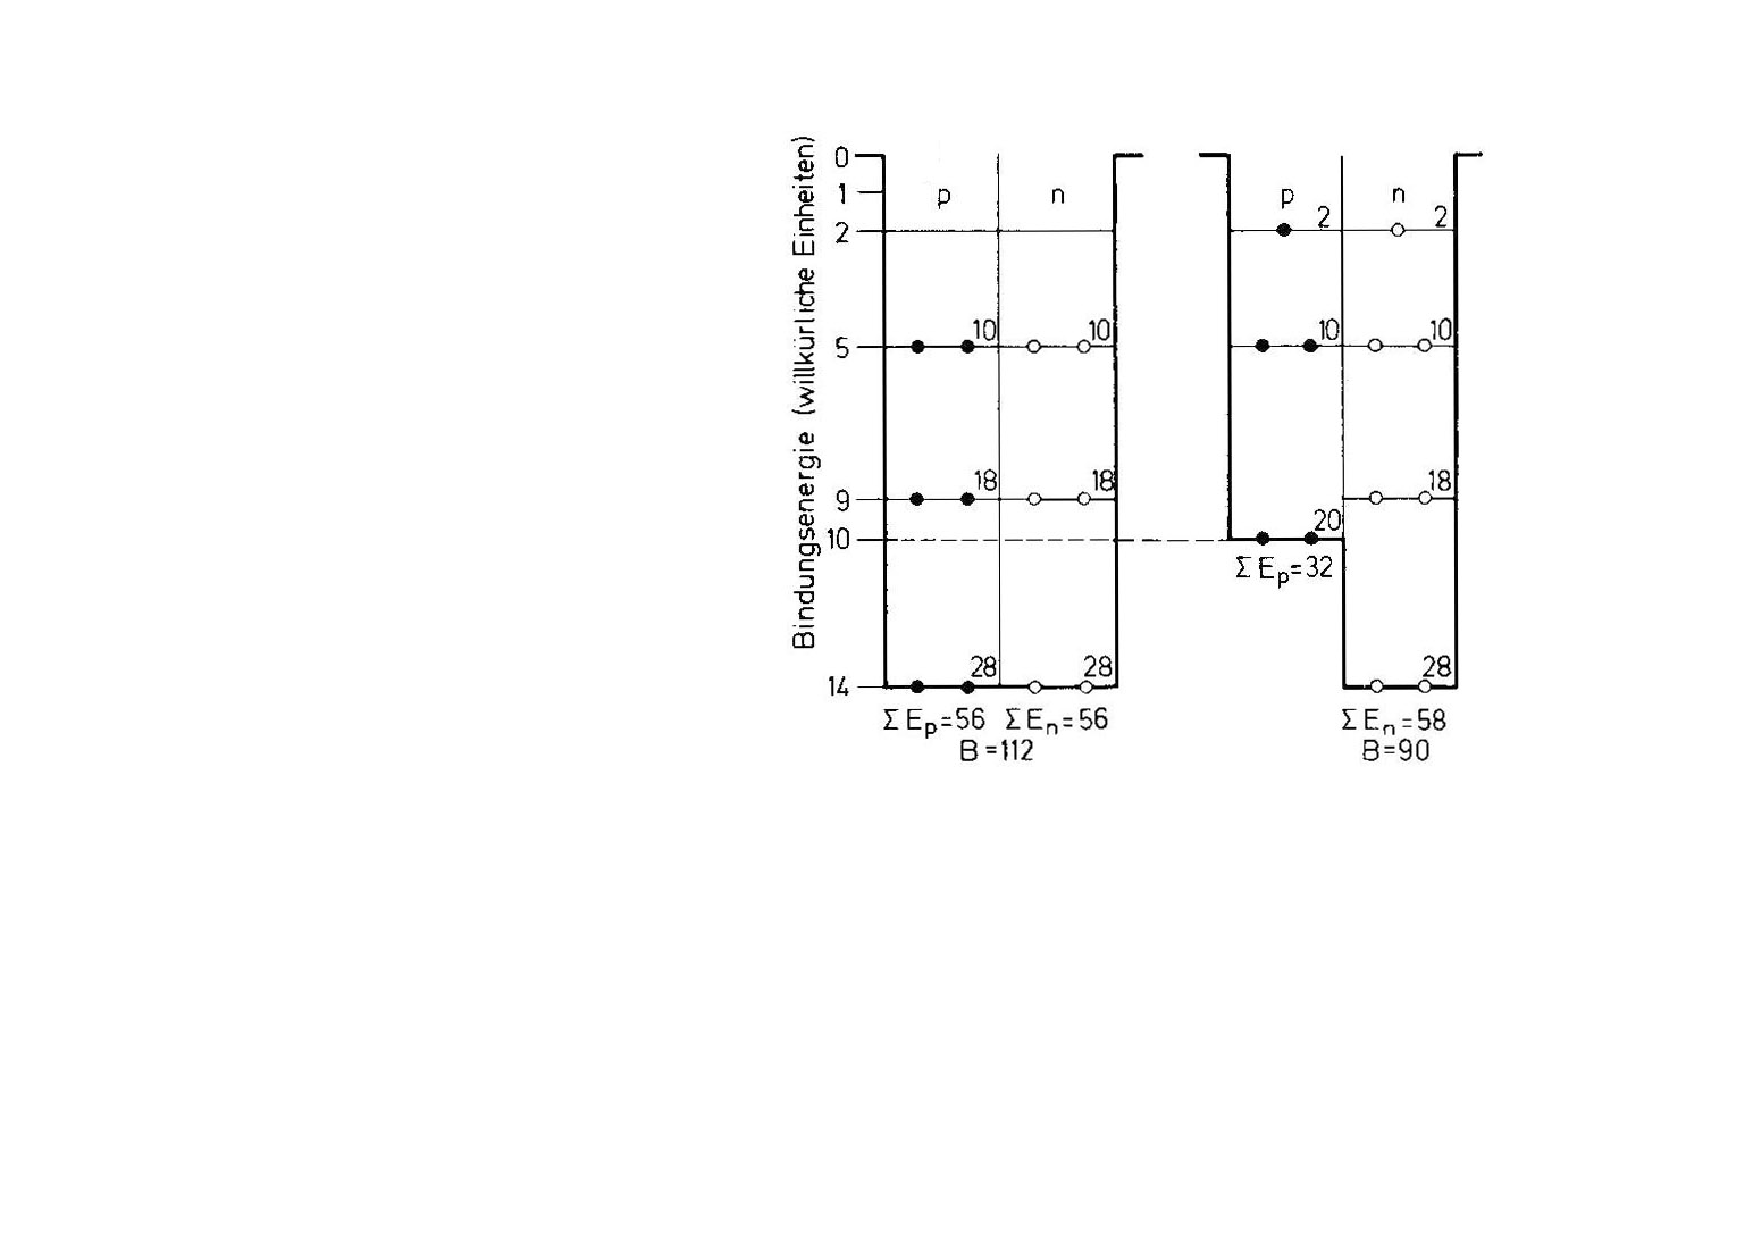
\includegraphics[width=0.8\textwidth]{fig/2-BindungsEnergieMitCoulombPotOhneCoulombPot.pdf}
% 	\caption{Vergleich der Bindungsenergie im symmetrischen (links) und
% 	unsymmetrischen Fermipotential (rechts)}
% \end{figure}

\item Man kann die Schalenstruktur der Kerne anfänglich so erklären, dass man
zum Einfügen eines Fermions in ein ``halb'' gefülltes Niveau kaum Energie
benötigt. Für leichte Kerne erhalten wir jedoch auch durch diese Annahme noch
kein hinreichendes Modell.
\item
Unser Modell ist in keinster Weise vollständig. Man könnte beispielsweise 
anstatt einem Potential mit scharfer Kante eines mit kontinuierlichem Verlauf
annehmen (sog. Wood-Saxon-Potential siehe Abb. \ref{fig:radlad}) und so zu
verbesserten Ergebnissen kommen. Wir werden jedoch sehen, dass das bisher entwickelte Modell für unsere Vorhaben $A>40$ hinreichend
genaue Aussagen macht.\maphere
\end{enumerate}
\end{bemn}

\subsubsection{Tröpfchenmodell}

Das \emph{Tröpfchenmodell} ist ein effektives Modell das auf einer
inkompressiblen Flüssigkeit, die durch kurzreichweitige Wechselwirkung
zusammengehalten wird, basiert. Es kann keine Aussage über die Peaks der
Bindungsenergie pro Nukelon im Bereich weniger Nukleonen machen, dafür
beschreibt es die Gesamtverteilung sehr genau.

Wir werden nun 5 Energien analysieren, die jeweils einen Beitrag zu
Bindungsenergie pro Nukelon leisten, d.h. es gilt
\begin{align*}
E_B = B_1 + B_2 + B_3 + B_4 + B_5.
\end{align*}


\sfigure[!htpb][1]%
	{2-EnergieTermeBWFormel.pdf}
	{\BethgeWalter, S. 49}
	{Bindungsenergie pro Nukleon als Funktion der Massenzahl.}
% 	
% \begin{figure}[!htbp]
% 	\centering
% 	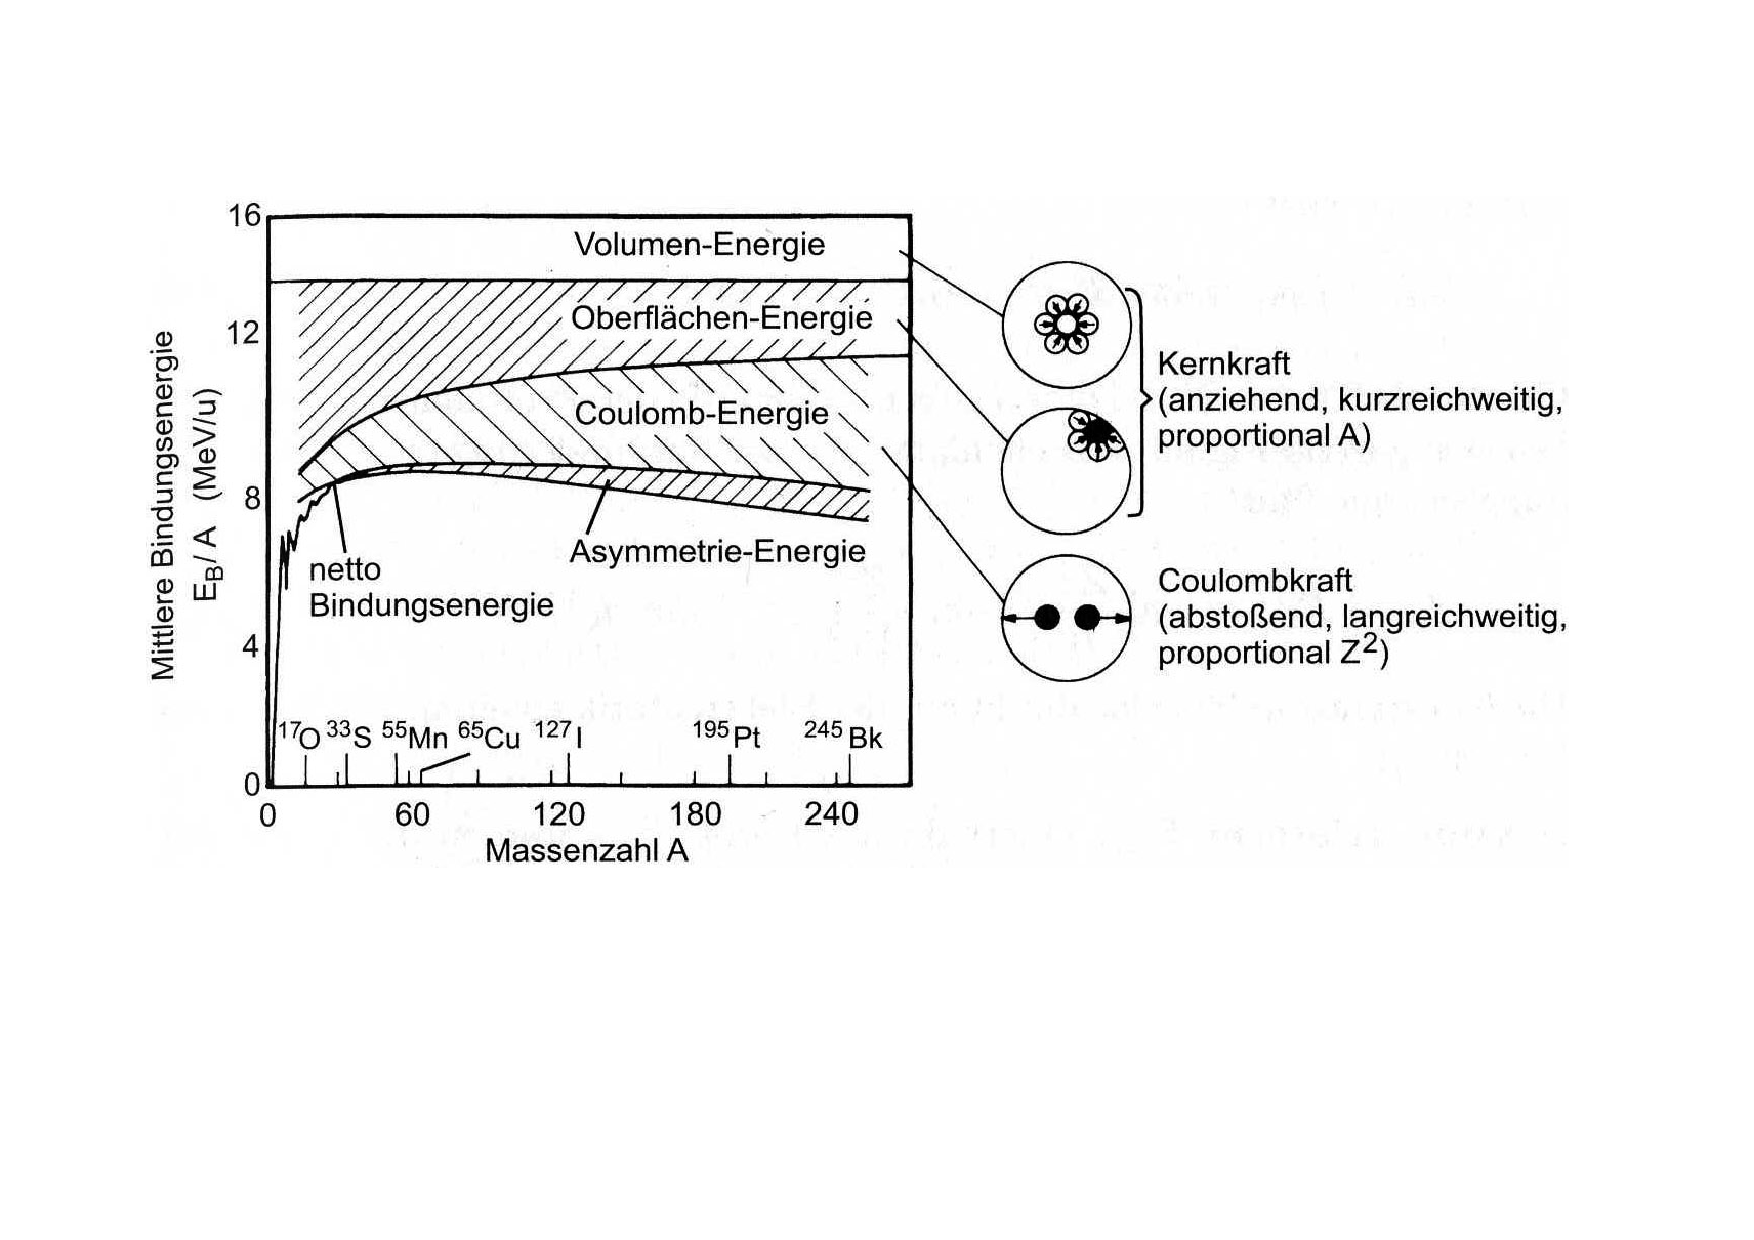
\includegraphics[width=\textwidth]{fig/2-EnergieTermeBWFormel}
% \end{figure}

\begin{enumerate}[label=\arabic{*}.)]
  \item Volumenenergie (Kondensationsenergie)

Wir haben bereits gesehen, dass das Volumen linear in der Nukleonenzahl $A$
ist, d.h.
\begin{align*}
B_1 = a_V A.%,\quad a_V = \frac{B}{A} = \const.
\end{align*}
\item Oberflächenenergie (Oberflächenspannung)

Die Oberfläche $S = 4\pi r_0^2\left(A^{1/3}\right)^2$ nimmt nicht linear mit der
Nukleonenzahl zu,
\begin{align*}
B_2 = -a_S A^{2/3},
\end{align*}
d.h. die Bindungsenergie wird \textit{größer}, wenn sich die Oberfläche
verkleinert.
\item Coulombenergie.

Die Coulombenergie einer homogen geladenen Kugel ist gegeben durch,
\begin{align*}
E = \frac{3}{5}\frac{q^2}{R},
\end{align*}
wobei $R = r_0 A^{1/3}$. Hier leisten nur die postiv geladenen Fermionen einen
Beitrag,
\begin{align*}
B_3 = -a_C \frac{Z^2}{A^{1/3}} = a_C Z^2 A^{-1/3}.
\end{align*}
\item Asymetrieenergie

Die Asymetrieenergie hat ihren Ursprung in der Coulomb-Wechselwirkung, denn
diese führt zum Neutronenüberschuss. Dadurch ändert sich die Zustandsdichte,
was im Fermimodell einer Änderung der Bindungsenergie pro Nukelon hervorruft.

Die Energie im Fermigas mit $n$ Fermionen lässt sich wie folgt abschätzen,
\begin{align*}
E_\tot = \int\limits_0^{E_F} 2E\frac{\dn}{\dE}\dE
\sim V\int\limits_{0}^{E_F} E^{\frac{3}{2}}\dE \sim VE^{\frac{5}{2}}
\sim V\left(\left(\frac{n}{V}\right)^{\frac{2}{3}} \right)^{\frac{5}{2}}
= A^{-\frac{2}{3}}n^{\frac{5}{3}}.
\end{align*}

Ein Atom enthält zwei Arten von Fermionen ($p^+,n^0$), es gilt somit
\begin{align*}
E_\tot = CA^{-\frac{2}{3}}\left(Z^{\frac{5}{3}} + N^{\frac{5}{3}}\right).
\end{align*}
Für einen symmetrischen Kern $N=Z$ erhalten wir so,
\begin{align*}
E_\tot = 2CA^{-\frac{2}{3}}\left(\frac{A}{2}\right)^{\frac{5}{3}} =
\frac{C}{2^{\frac{2}{3}}}A.
\end{align*}
Wie viel Energie kostet von dieser Energie aus ein Neutronenüberschuss $T_Z =
\frac{1}{2}(Z-N)$?
\begin{align*}
\Delta E = CA^{-\frac{2}{3}}\left(Z^{\frac{5}{3}} + N^{\frac{5}{3}} -
2\left(\frac{A}{2}\right)^{\frac{5}{3}}\right)
\end{align*}
Da die Gesamtenergie nicht linear in $n$ ist, ist die Energiedifferenz nicht
Null. Wir wollen $\Delta E$ für keines $T_Z$ entwickeln,
\begin{align*}
\Delta E &= CA^{-\frac{2}{3}}\left(\left(\frac{A}{2} + T_Z\right)^{\frac{5}{3}}
+ \left(\frac{A}{2} - T_Z\right)^{\frac{5}{3}} -
2\left(\frac{A}{2}\right)^{\frac{5}{3}}\right)\\ &
= 2^{-\frac{5}{3}}CA^{-\frac{2}{3}}A^{\frac{5}{3}}\left(
\left(1+\frac{2T_Z}{A}\right)^{\frac{5}{3}}
+\left(1-\frac{2T_Z}{A}\right)^{\frac{5}{3}}
-2 \right).
\end{align*}
Verwende $(1\pm x)^{p} = 1\pm px + \frac{p(p-1)}{2}x^2 + \ldots$,
\begin{align*}
&\Delta E = 2^{-\frac{5}{3}}CA^{-\frac{2}{3}}A^{\frac{5}{3}}\left(
2  + 2\frac{4}{A^2}\frac{10}{9}T_Z^2 - 2\right) = 2^{-\frac{2}{3}}
\frac{80}{9}\frac{T_Z^2}{A},\\ \Rightarrow & B_4 = -a_A \frac{T_Z^2}{A} =
-a_A\frac{\left(Z-\frac{A}{2}\right)^2}{A}
\end{align*}
\item Paarbildungsenergie.

Die Paarbildungsenergie muss empirisch eingeführt werden, um der Beobachtung
gerecht zu werden. Betrachten wir die Neutronen und Protonen Energiniveaus, so
können die jeweils gerade (g) oder ungerade (u) besetzt sein. Die
Beobachtung zeigt, dass (gg) Kerne besonders stabil und (uu) Kerne weniger
gebunden sind. Es ist energetisch günstig ein Nukelon in ein bereits halb
besetztes Energieniveau einzufügen.

Wir wollen dies durch folgenden Term berücksichtigen.
\begin{align*}
B_5 = \begin{cases}      
+\delta, & \text{für gg},\\
0, & \text{für ug/gu},\\
-\delta, & \text{für uu}.
\end{cases}
\end{align*} 
\end{enumerate}
Alle fünf Terme zusammen führen zur \emph{Bethe-Weizsäcker-Formel} mit der sich
die Bindungsenergie pro Nukelon vorhersagen lässt,
\begin{align*}
&E_B = B_1 + B_2 + B_3 + B_4 + B_5
= a_V A -a_S A^{2/3}-a_C
\frac{Z^2}{A^{1/3}}-a_A\frac{\left(Z-\frac{A}{2}\right)^2}{A}\pm \delta,\\
& m(Z,N) = N\cdot m_{n^0} + Z m_{p^+} - \frac{E_B}{c^2}. 
\end{align*}
Für schwere Kerne erreicht die Formel eine Präzission von einem Prozent. Wir
werden sehen, dass wir sogar Kernzerfälle mithilfe dieser Formel vorhersagen
können.

\noindent\textit{Interpretation der Bethe-Weizsäcker-Formel.}
%\begin{bemn}[]
\begin{enumerate}[label=\arabic{*})]
  \item Das Maximum der Bindungsenergie pro Nukleon $\frac{B}{A}$ kommt durch
  die Abnahme der Oberflächenenergie und der Zunahme der Coulombenergie
  zustande.
  \item Schaleneffekte für kleine $A$ werden nicht berücksichtig. Für $A>40$
  beschreibt die Formel $\frac{B}{A}$ jedoch auf 1 Prozent genau.
  \item Mithilfe der Formel lassen sich Aussagen über die Stabilität der Kerne machen.
  
  Betrachten wir Isobare, d.h. $A=\const$, in der Nähe von $N(Z,A)\sim Z^2$.
  Für $A$ ungerade erhalten wir folgendes Zerfallsschema.
\begin{figure}[H]
  \centering
\begin{pspicture}(1,-1.5)(7,1.5)
\psaxes[labels=none,ticks=none]{->}%
(4,-0.75)(1.6,-0.95)(6.4,1.25)[\color{gdarkgray}$Z$,-90][\color{gdarkgray}$m$,0]
\psbezier(1.86,0.7981994)(2.26,-1.2798958)(5.776432,-1.2598958)(6.16,0.90010417)
\pscircle[fillstyle=solid,fillcolor=white](2.78,-0.29989582){0.12}
\pscircle[fillstyle=solid,fillcolor=white](2.06,0.54010415){0.12}
\pscircle[fillstyle=solid,fillcolor=gdarkgray](4.0,-0.6198958){0.12}
\pscircle[fillstyle=solid,fillcolor=white](5.18,-0.29989582){0.12}
\pscircle[fillstyle=solid,fillcolor=white](5.9,0.54010415){0.12}
\psbezier[linecolor=darkblue,linestyle=dotted,dotsep=0.06cm]{->}(2.18,0.36010417)(2.3,0.10010417)(2.4,0.020104166)(2.62,-0.15989584)
\psbezier[linecolor=darkblue,linestyle=dotted,dotsep=0.06cm]{->}(2.98,-0.39989585)(3.24,-0.57989585)(3.48,-0.59989583)(3.84,-0.6198958)
\psbezier[linecolor=yellow,linestyle=dotted,dotsep=0.06cm]{->}(5.02,-0.39989585)(4.76,-0.57989585)(4.52,-0.59989583)(4.16,-0.6198958)
\psbezier[linecolor=yellow,linestyle=dotted,dotsep=0.06cm]{->}(5.82,0.36010417)(5.7,0.10010417)(5.6,0.020104166)(5.38,-0.15989584)

\rput(3.7626562,-1.0098958){\color{gdarkgray}$Z_0$}
\rput(5.5242186,0.35010415){\color{gdarkgray}$\beta^+$}
\rput(4.624219,-0.26989582){\color{gdarkgray}$\beta^+$}
\rput(3.3042188,-0.26989582){\color{gdarkgray}$\beta^-$}
\rput(2.5242188,0.31010416){\color{gdarkgray}$\beta^-$}
\end{pspicture} 
  \caption{Zerfallsschema für Isobare mit $A$ ungerade. Stabiler Kern ist
  ausgefüllt.}
\end{figure}
  Wir können somit konkret ausrechnen, welche Energie die Elektronen beim
  $\beta$-Zerfall haben.
  
 \begin{figure}[!ht]
  \centering
\begin{pspicture}(0.5,-1.65)(7.5,2)
\psaxes[labels=none,ticks=none]{->}%
(4,-0.95)(1,-1)(7,1.7)%
[\color{gdarkgray}$Z$,-90][\color{gdarkgray}$m$,0]

\psbezier(1.14,0.590077)(1.6832558,-1.5070833)(6.459061,-1.4868999)(6.98,0.6929167)
\pscircle[fillstyle=solid,fillcolor=white](3.0,0.91291666){0.12}
\pscircle[fillstyle=solid,fillcolor=gdarkgray](1.44,0.19291666){0.12}
\pscircle[fillstyle=solid,fillcolor=gdarkgray](4.0,-0.82708335){0.12}
\pscircle[fillstyle=solid,fillcolor=white](5.16,0.91291666){0.12}
\pscircle[fillstyle=solid,fillcolor=gdarkgray](6.62,0.19291666){0.12}

\psbezier(2.02,1.5910119)(3.12,0.19291666)(5.06,0.17291667)(6.32,1.6929166)
\psline[linecolor=yellow,linestyle=dotted,dotsep=0.06cm]{->}(5.4,0.7729167)(6.46,0.25291666)
\psline[linecolor=darkblue,linestyle=dotted,dotsep=0.06cm]{->}(5.0,0.61291665)(4.2,-0.64708334)
\psline[linecolor=yellow,linestyle=dotted,dotsep=0.06cm]{->}(2.66,0.7529167)(1.6,0.23291667)
\psline[linecolor=darkblue,linestyle=dotted,dotsep=0.06cm]{->}(3.06,0.59291667)(3.86,-0.6670833)

\rput(3.7626562,-1.2170833){\color{gdarkgray}$Z_0$}
\rput(6.981406,0.1){\color{gdarkgray}\small$gg$}
\rput(1,0.1){\color{gdarkgray}\small$gg$}
\rput(2.8595312,1.28){\color{gdarkgray}\small$uu$}
\rput(5.4195313,1.28){\color{gdarkgray}\small$uu$}
\psline[linestyle=dotted,dotsep=0.06cm]{->}(1.6,0.09291667)(3.76,-0.8070833)
\psline(2.68,-0.18708333)(2.44,-0.40708333)
\psline[linestyle=dotted,dotsep=0.06cm]{->}(6.42,0.11291666)(4.26,-0.7870833)
\psline(5.34,-0.16708334)(5.58,-0.38708332)

\rput(1.9242188,0.7029167){\color{gdarkgray}$\beta$}
\rput(3.5042188,0.24291667){\color{gdarkgray}$\beta$}
\rput(4.5642185,0.24291667){\color{gdarkgray}$\beta$}
\rput(6.144219,0.7029167){\color{gdarkgray}$\beta$}
\end{pspicture} 
  \caption{Zerfallsschema für Isobare mit $A$ gerade. Stabile Kerne sind
  ausgefüllt.}
\end{figure}

 Für $A$ gerade ist $\Delta p^+ = 2k$, um von einem gg zu einem anderen gg zu
 kommen. Es gibt jedoch keinen $\beta$-Zerfall bei dem sich die
 Protonenzahl um ein Vielfaches von $2$ ändert. Daher gibt es viele stabile
 $gg$ Isotope.
\item Man kann mit der Formel auch die stabilsten Kerne vorhersagen, indem man
 die Bindungsenergie maximiert.
\begin{align*}
\frac{\partial m(Z,A=Z+N)}{\partial Z}\bigg|_{N=\const} = 0.
\end{align*}
% 
% \begin{figure}[!htbp]
% 	\centering
% 	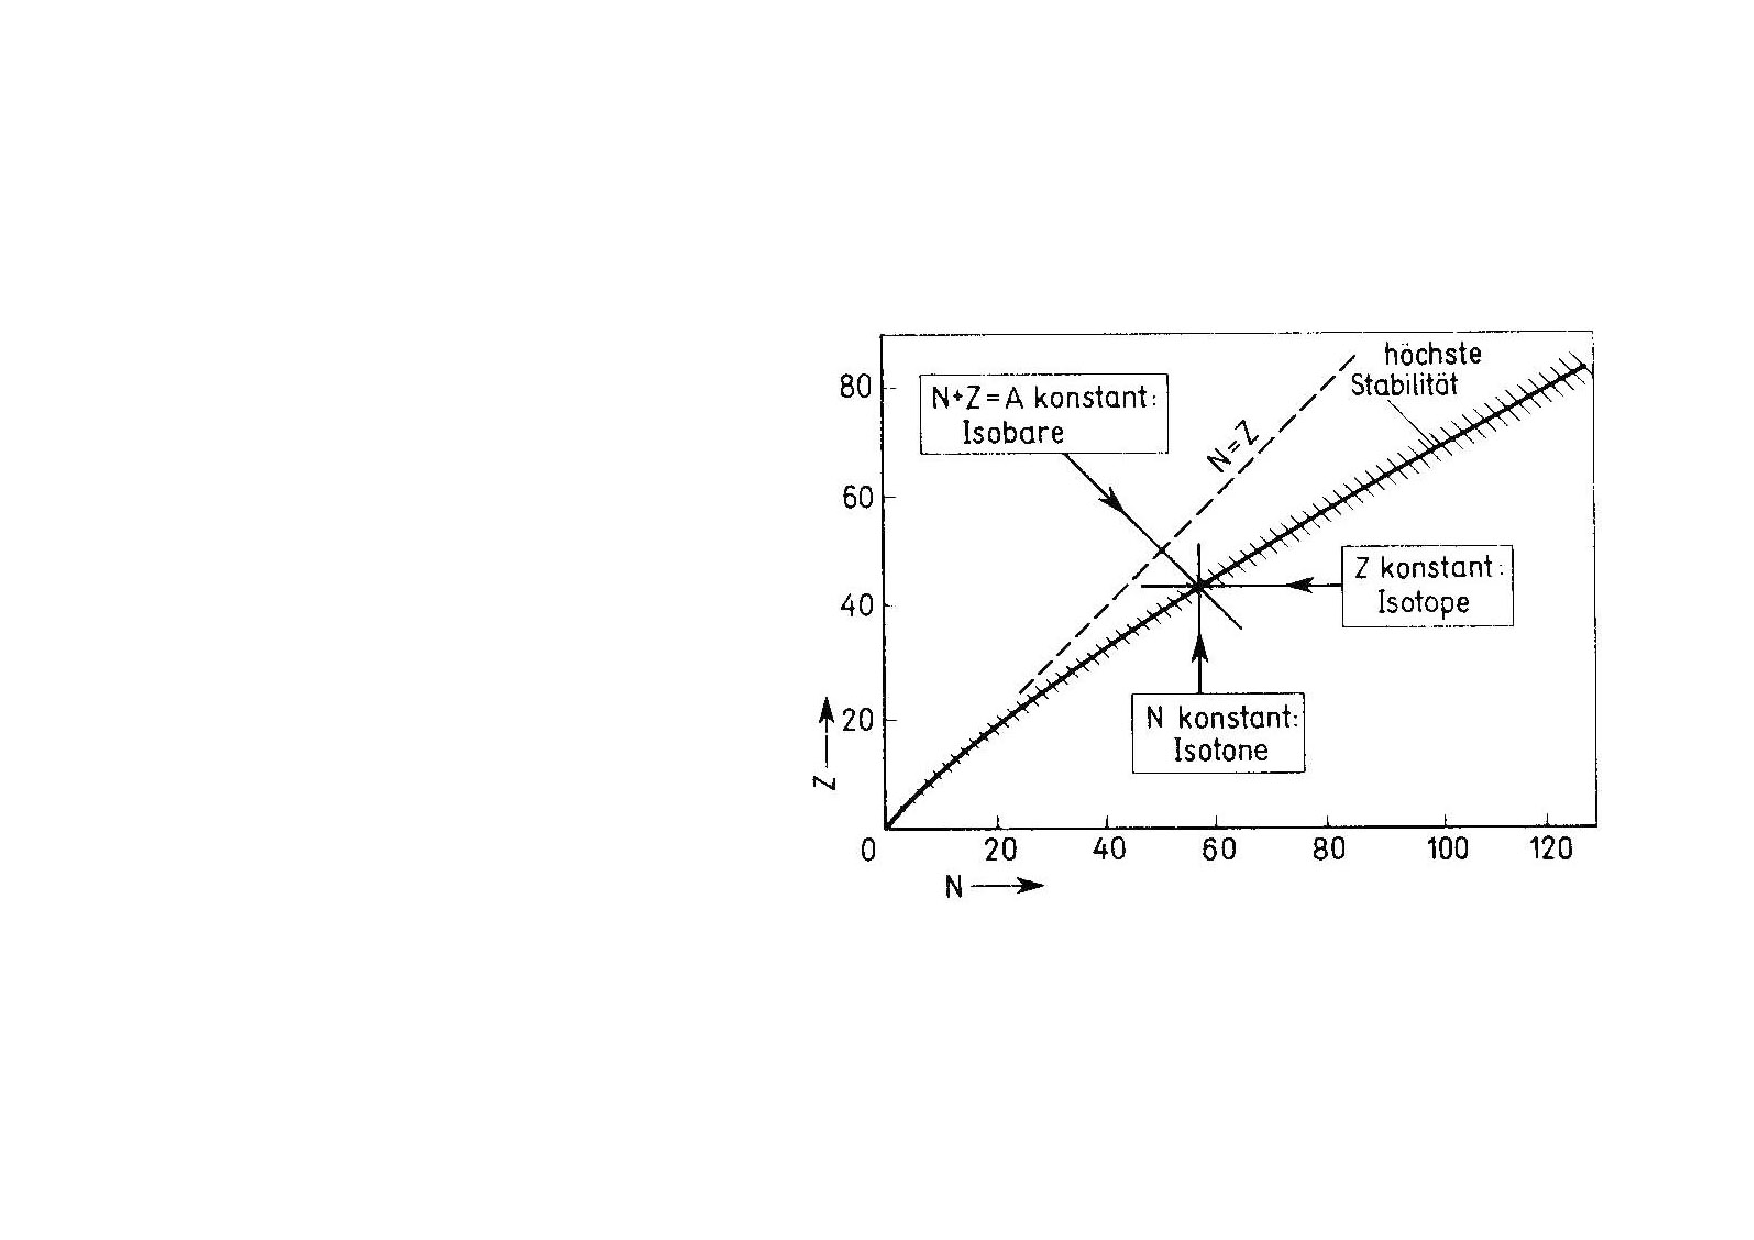
\includegraphics[width=0.9\textwidth]{fig/2-LageStabileKerneNZEbene.pdf}
% \end{figure}


\sfigure[!htpb][0.5]%
	{2-LageStabileKerneNZEbene.pdf}
	{\KuckukKern, S. 53}
	{Lage der stabilen Kerne in der $N$-$Z$-Ebene.}

\item
Beim $\alpha$-Zerfall wird ein $He$-Kern $(2p^+,2n^0)$ emittiert,
\begin{align*}
{}_Z^A  X \overset{\alpha}{\longrightarrow} {}_{Z-2}^{A-4} X + \alpha^{2+}.
\end{align*}
Die Energiebilanz des $\alpha$-Zerfalls ist,
\begin{align*}
E_\alpha = \left[m(Z,A) - m(Z-2,A-4) - m_\alpha\right]c^2.
\end{align*}
Für $E_\alpha > 0$ ist der Zerfall möglich, für wachsendes $E_\alpha$ wird der
Prozess schneller. Man kann dies mit dem Modell von Gamov
beschreiben.
\begin{figure}[!ht]
  \centering
% Generated with LaTeXDraw 2.0.3
% Mon Jul 13 20:26:46 CEST 2009
% \usepackage[usenames,dvipsnames]{pstricks}
% \usepackage{epsfig}
% \usepackage{pst-grad} % For gradients
% \usepackage{pst-plot} % For axes
\scalebox{1} % Change this value to rescale the drawing.
{
\begin{pspicture}(0,-1.78)(4.4,1.78)
\psbezier(1.3941112,0.435)(1.3941112,1.115)(1.36,1.56)(1.5,1.56)(1.64,1.56)(1.82,1.32)(2.08,1.04)(2.34,0.76)(2.72,0.4)(3.9,0.4)
\psline(1.3941112,0.495)(1.374111,-1.405)(0.014111111,-1.405)(0.0,1.72)
\pscircle(0.6341111,1.255){0.22}
\psline[linestyle=dotted,dotsep=0.06cm]{->}(1.0341111,1.22)(3.82,1.22)
\psline{->}(1.38,0.4)(4.28,0.4)
\psline(1.92,1.2)(1.92,0.4)
\psdots[dotsize=0.12](0.12,-1.4)
\psdots[dotsize=0.12](0.52,-1.4)
\psdots[dotsize=0.12](0.12,-1.0)
\psdots[dotsize=0.12](0.52,-1.0)
\psdots[linecolor=darkblue,dotsize=0.12](0.12,0.6)
\psdots[linecolor=darkblue,dotsize=0.12](0.52,0.6)
\psdots[dotsize=0.12](0.12,-0.6)
\psdots[dotsize=0.12](0.52,-0.6)
\psdots[dotsize=0.12](0.12,-0.2)
\psdots[dotsize=0.12](0.52,-0.2)
\psdots[dotsize=0.12](0.12,0.2)
\psdots[dotsize=0.12](0.52,0.2)
\psdots[linecolor=yellow,dotsize=0.12](0.88,0.6)
\psdots[linecolor=yellow,dotsize=0.12](1.28,0.6)
\psdots[dotsize=0.12](0.88,0.36)
\psdots[dotsize=0.12](1.28,0.36)
\psdots[dotsize=0.12](0.88,0.1)
\psdots[dotsize=0.12](1.28,0.1)
\psdots[dotsize=0.12](0.88,-0.2)
\psdots[dotsize=0.12](1.28,-0.2)
\psdots[dotsize=0.12](0.88,-0.54)
\psdots[dotsize=0.12](1.28,-0.54)
\psdots[dotsize=0.12](0.88,-0.88)
\psdots[dotsize=0.12](1.28,-0.88)

\psline{->}(0.62,0.7)(0.62,1.02)
\psline{<->}(3.52,1.18)(3.52,0.44)

\rput(1.55,0.225){\color{gdarkgray}$r_1$}
\rput(2.09,0.225){\color{gdarkgray}$r_2$}
\rput(0.31,-1.575){\color{gdarkgray}$n$}
\rput(1.09,-1.555){\color{gdarkgray}$p$}
\rput(0.62,1.665){\color{gdarkgray}$\alpha$}
\rput(3.92,0.765){\color{gdarkgray}$E_\kin$}
\rput(4.3,0.225){\color{gdarkgray}$r$}
\end{pspicture} 
}

  \caption{Gamovs Erklärung des $\alpha$-Zerfalls.}
\end{figure}

Damit der $\alpha$-Zerfall stattfindet, muss das im Kern entstehende
$\alpha$-Teilchen eine große Barriere, hervorgerufen durch die starke
Kernbindung, überwinden. Kann dadurch Energie frei werden, so existiert eine
bestimmte Wahrscheinlichkeit, dass das Teilchen durch die Barriere tunnelt.
Nach dem Tunneln erhält das $\alpha$-Teilchen eine große kinetische Energie
und kann aufgrund der Barriere nicht mehr in den Kern
zurückkehren. Für die Tunnelwahrscheinlichkeit gilt,
\begin{align*}
\text{Wsk} \sim \exp\left\{\text{Freiwerdende Energie}\right\}.
\end{align*}
\item Die Formel erklärt ebenfalls, warum nur $\alpha$- und $\beta$-Zefälle
auftreten und nicht etwa nur $p^+$ oder $n^0$ emittiert werden. Da
das $\alpha$-Teilchen bereits eine sehr hohe Bindungsenergie hat, ist es
in den meisten Fällen die günstigste Zerfallsvariante. In der Formel ist eine
Änderung von $Z$ oder $N$ um 1 stets ungünstiger als der $\alpha$-Zerfall.
\item Auch für die Kernspaltung kann mit der Bethe-Weizsäcker-Formel eine
Energiebilanz aufgestellt werden. Gilt
\begin{align*}
m(Z,A) > 2m\left(\frac{Z}{2},\frac{A}{2}\right),
\end{align*}
so ist die Spaltung energetisch möglich. Jedoch ist auch hier - wie beim
$\alpha$-Zerfall - eine Barriere zu überwinden.

% \begin{figure}[!htbp]
% 	\centering
% 	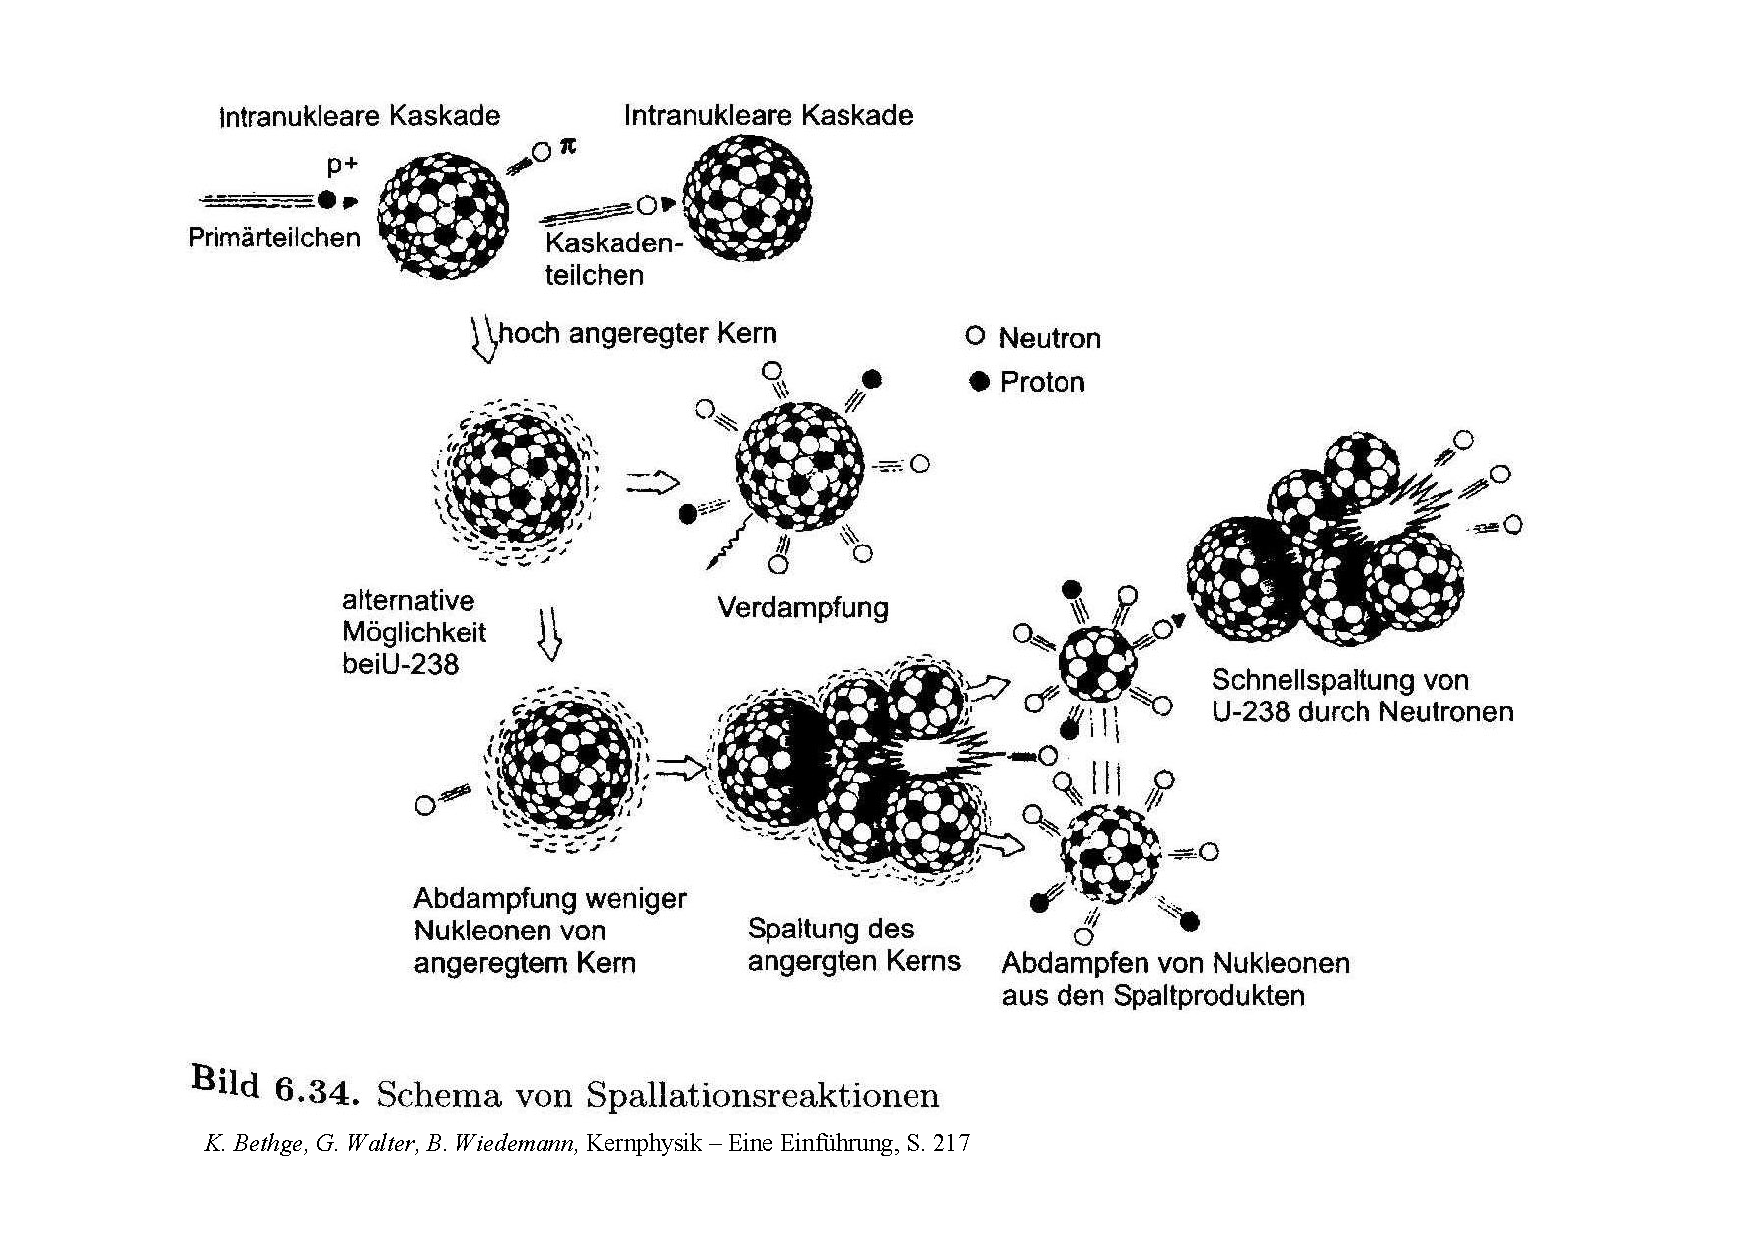
\includegraphics[width=0.9\textwidth]{fig/2-Kernspaltung.pdf}
% \end{figure}

 Man hat von zahlreichen
Nukleonen die Halbwertszeit $\tau_{1/2}$ bestimmt und stellte fest, dass
\begin{align*}
\tau_{1/2} \sim \frac{1}{\lambda},
\end{align*}
wobei $\lambda$ die Tunnelwahrscheinlichkeit des $\alpha$-Teilchens
bezeichnet. Diesen Zusammenhang nennt man die \emph{Geiger-Nuttall-Regel}. Im
Experiment sieht man eine Übereinstimmung über 25 Größenordnungen hinweg.
% 
% \begin{figure}[!htbp]
% 	\centering
% 	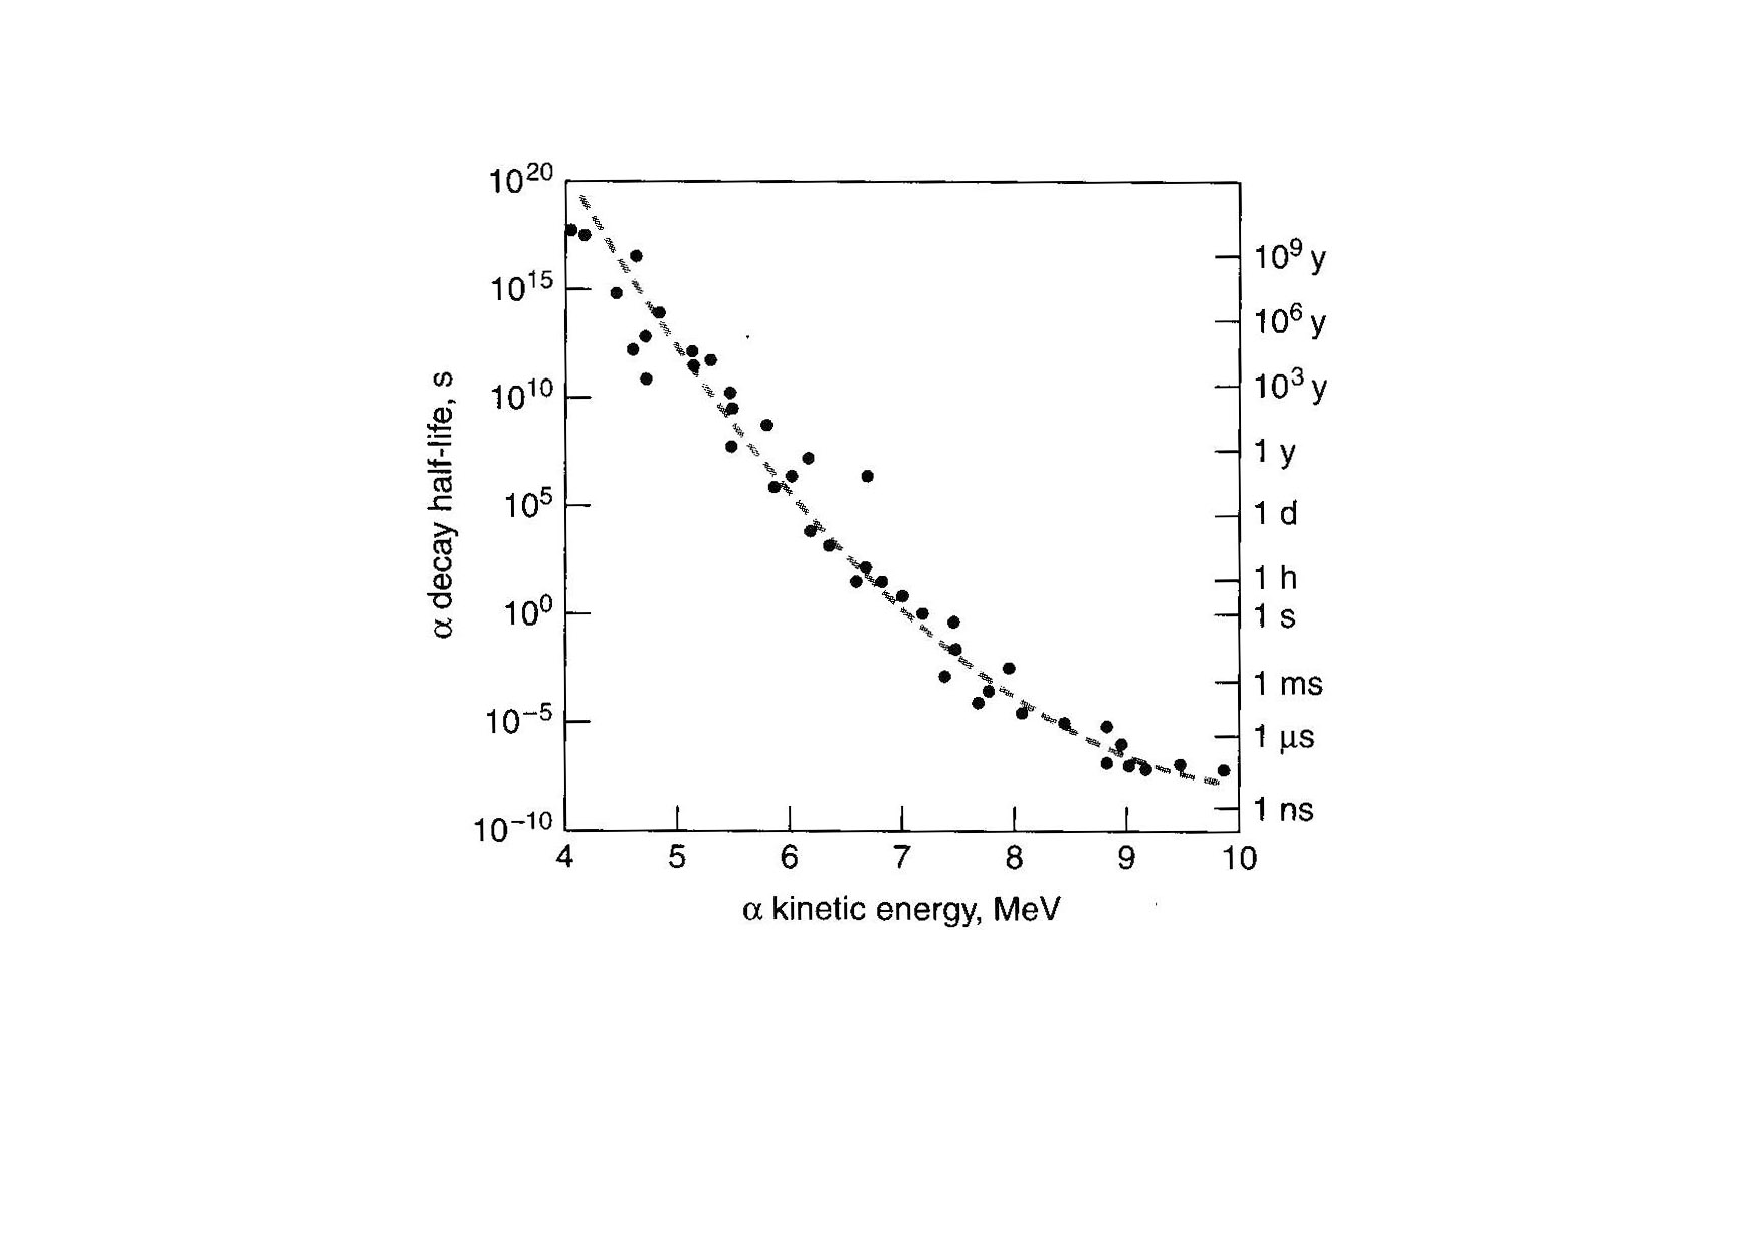
\includegraphics[width=0.9\textwidth]{fig/2-GeigerNuttallRegel.pdf}
% \end{figure}
% 

\sfigure[!htpb][0.7]%
	{2-GeigerNuttallRegel.pdf}
	{\TiplerMPFife, S. 496}
	{Halbwertszeit des $\alpha$-Zefalls
	für natürlich vorkommende Zerfälle halblogarithmisch über der kinetischen
	Energie der $\alpha$ Teilchens aufgetragen. Die gestrichelte Linie stellt die
	Vorhersage der Geiger-Nuttall Regl dar.}


Die Tunnelwahrscheinlichkeit für eine spontane Spaltung ist typischerweise
viel kleiner als die für den $\alpha$-Zerfall. Man kann jedoch durch 
Neutroneneinfang Energie in das System einbringen und dadurch die Spaltung
induzieren.

Der Kernspaltungsprozess zeigt Analogieen zur Verformung von elastischen
Körpern. Die für eine Spaltung zu überwindende Potentialbarriere ist in diesem
Modell vergleichbar mit einem Riss der Oberfläche.

\sfigure%
	{2-SpaltDeformation.pdf}
	{\BethgeWalter, S. 244}
	{Einfache (gestrichelt) und doppelhöckrige Spaltbarriere.}
% 
% \begin{figure}[!htbp]
% 	\centering
% 	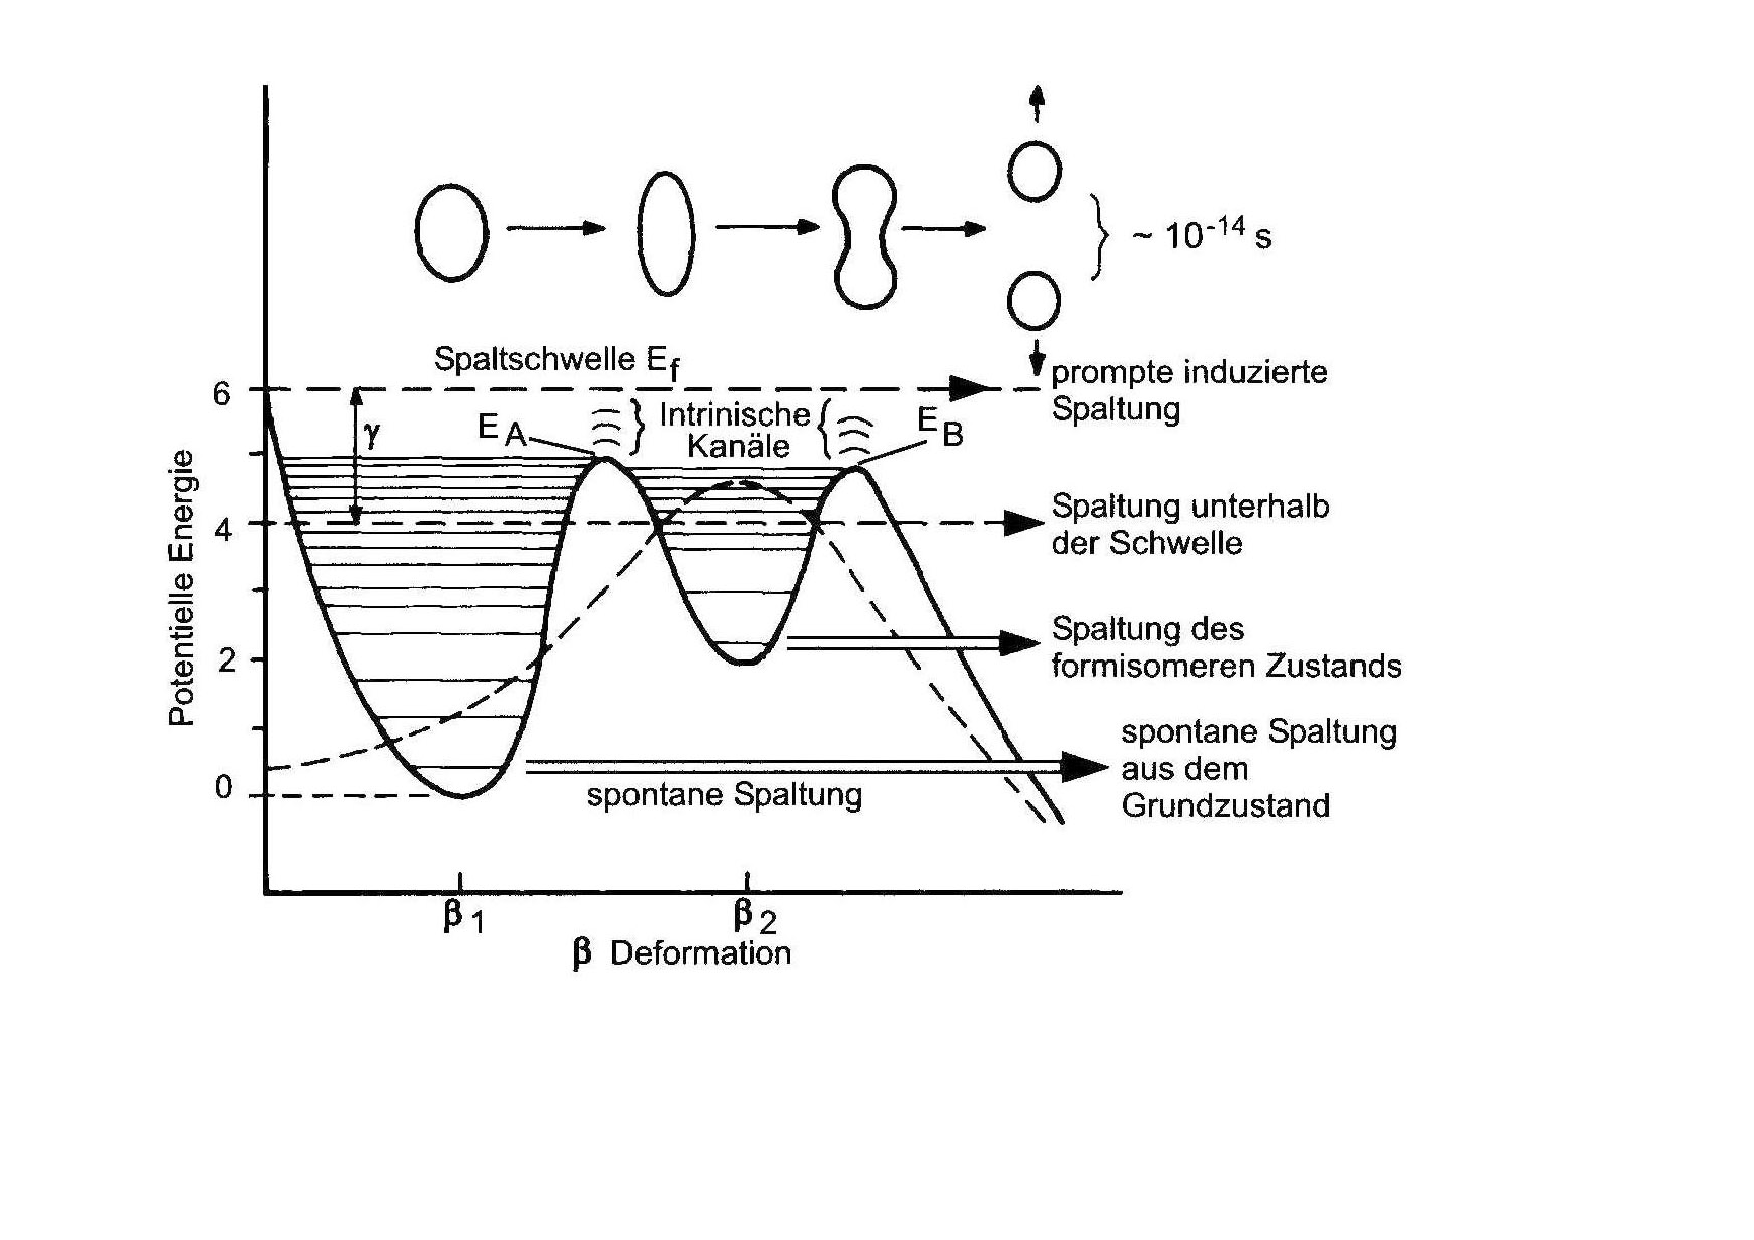
\includegraphics[width=\textwidth]{fig/2-SpaltDeformation.pdf}
% \end{figure}

\begin{bspn}
Bei Uran 235 ist die günstigste Spaltung nicht die Halbierung sondern die
Teilung in einem schweren $\sim 140\mathrm{u}$ und einen leichten $\sim
90\mathrm{u}$ Kern. Auch dies folgt aus der Bethe-Weizsäcker-Formel und ist für
viele weitere Kerne der Fall.\bsphere
\end{bspn}

% 	
% \begin{figure}[H]
% 	\centering
% 	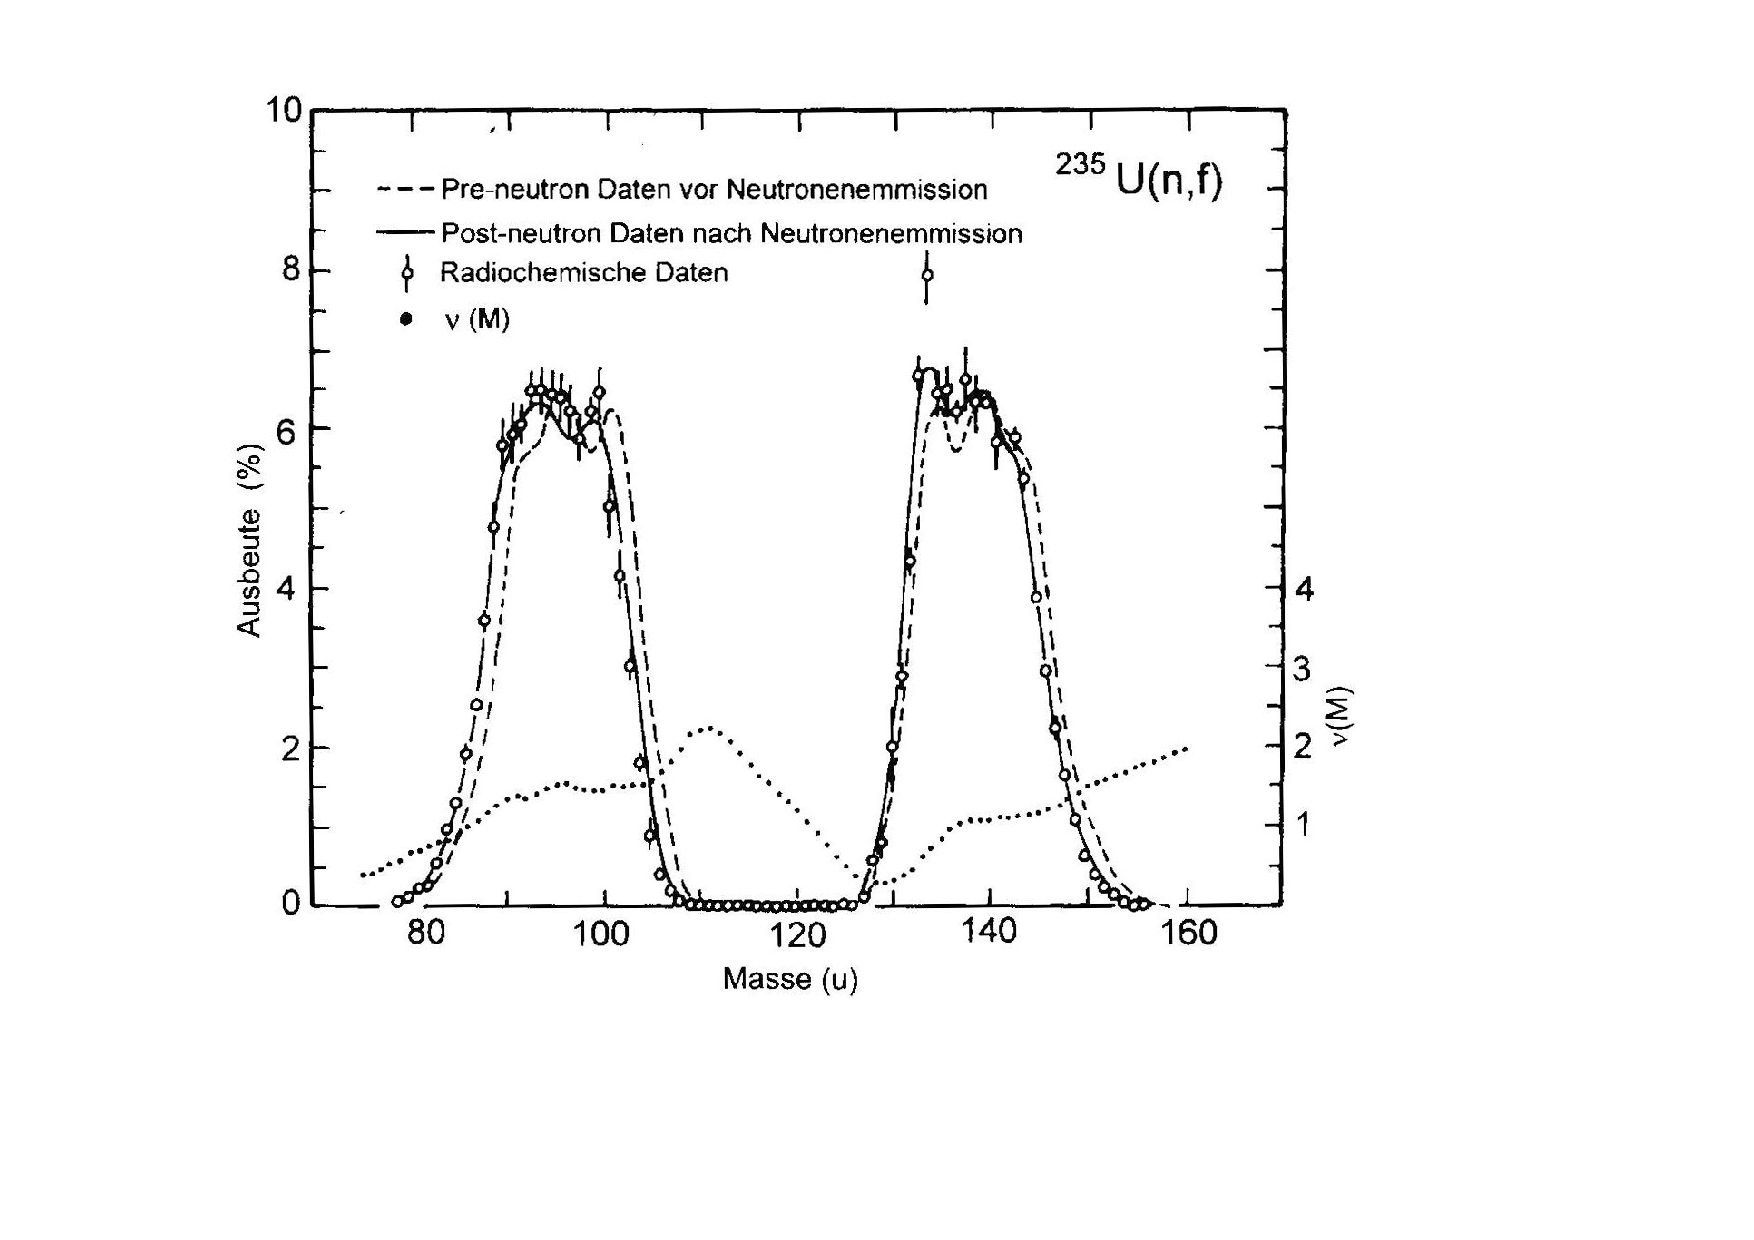
\includegraphics[width=\textwidth]{fig/2-MassenverteilungSpaltfragmenteUran.pdf}
% \end{figure}


\sfigure[H][0.7]%
	{2-MassenverteilungSpaltfragmenteUran.pdf}
	{\BethgeWalter, S. 240}
	{Massenverteilung der Spaltfragmente aus ${}^{235}\mathrm{U}(n,f)$. Die
	gepunktete Linie gibt die mittlere Anzahl der emittierten Neutronen $\nu(M)$
	aus.}
	
% 	\begin{figure}[!htbp]
% 	\centering
% 	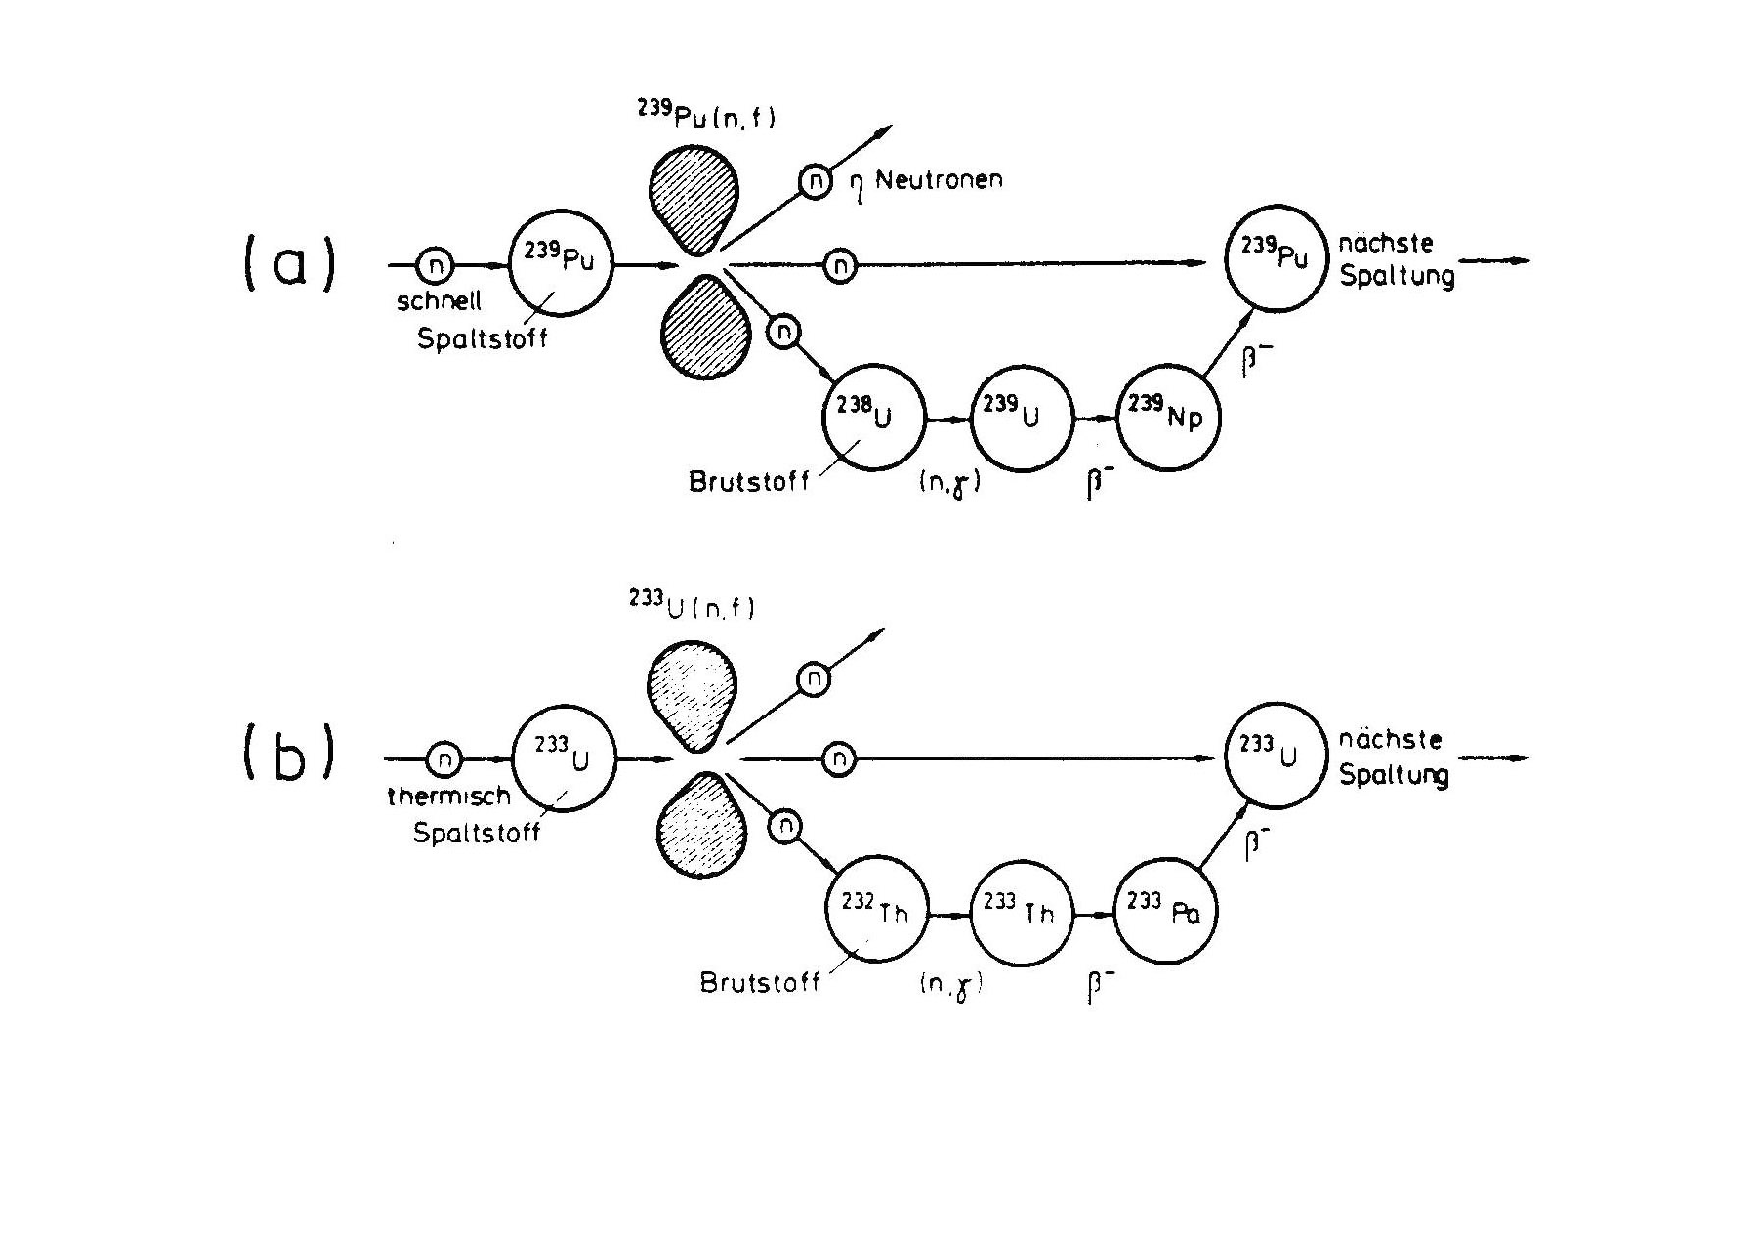
\includegraphics[width=\textwidth]{fig/2-SpaltBrutKetten.pdf}
% \end{figure}

\sfigure[H][0.7]%
	{2-SpaltBrutKetten.pdf}
	{\KuckukKern, Fig. 127}
	{Spalt-Brutketten. a) Schneller Brüter, b) Thorium-Brüter.}


\begin{bspn}
Berücksichtigt man zusätzlich noch die Schalenstruktur der Kerne, so lässt sich im Bereich
von $Z\sim 120$, $N\sim 190$ eine ``Insel der Stabilität'' vorhersagen, d.h. es
könnte dort bisher unentdeckte aber stabile Elemente geben. Es stellt sich jedoch als
äußerst schwierig heraus, diese
``Superschweren Kerne'' zu erzeugen.\bsphere
\end{bspn}


\sfigure[H]%
	{2-StabilitaetsGebirge.pdf}
	{\KuckukKern, Fig. 55}
	{Bindungsenergien der Kerne in Abhängigkeit von $Z$ und $N$. Nur die aus der
	Obefläche herausragenden Kerne sind stabil. Bei $N\approx 190$ befindet sich
	die spekulative Stabilitätsinsel.}

\begin{figure}[H]
	\centering
% 	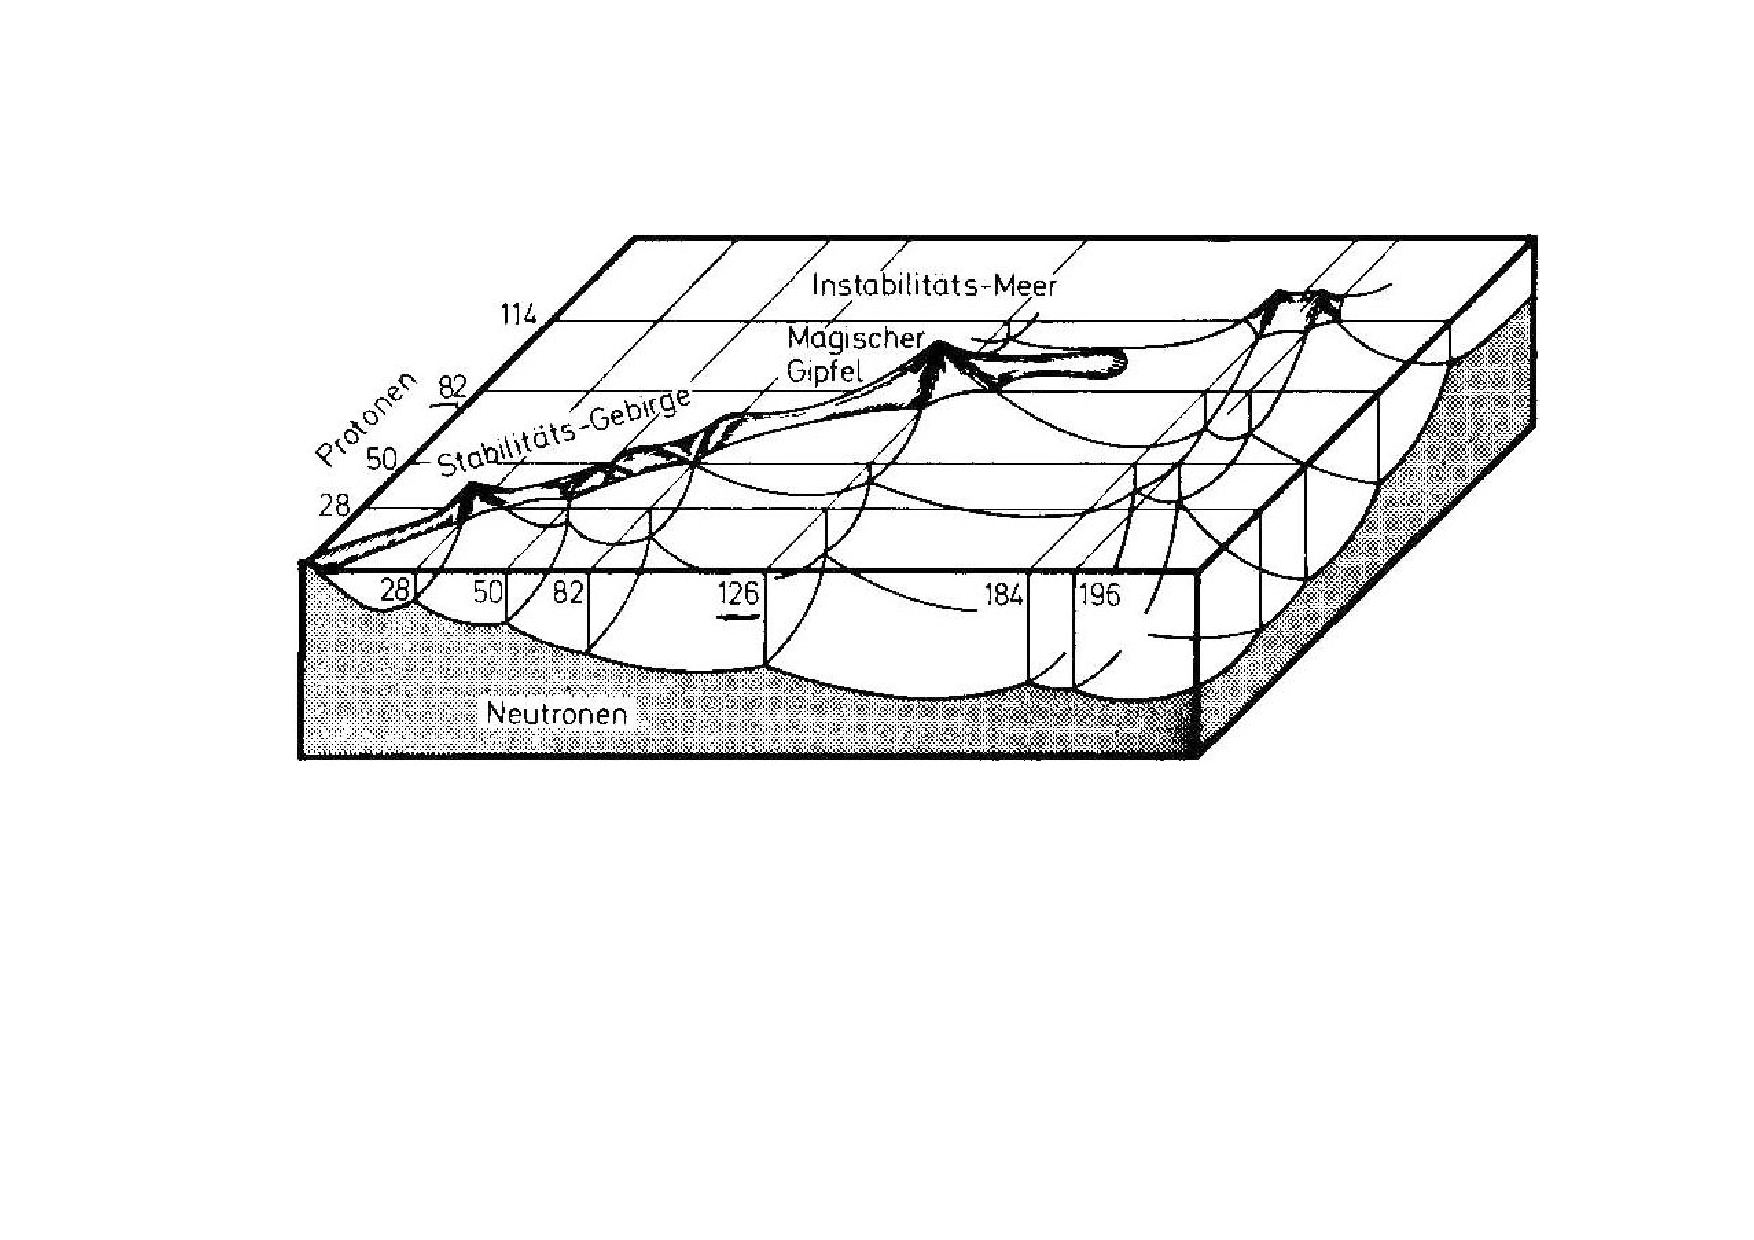
\includegraphics[width=\textwidth]{fig/2-StabilitaetsGebirge.pdf}
	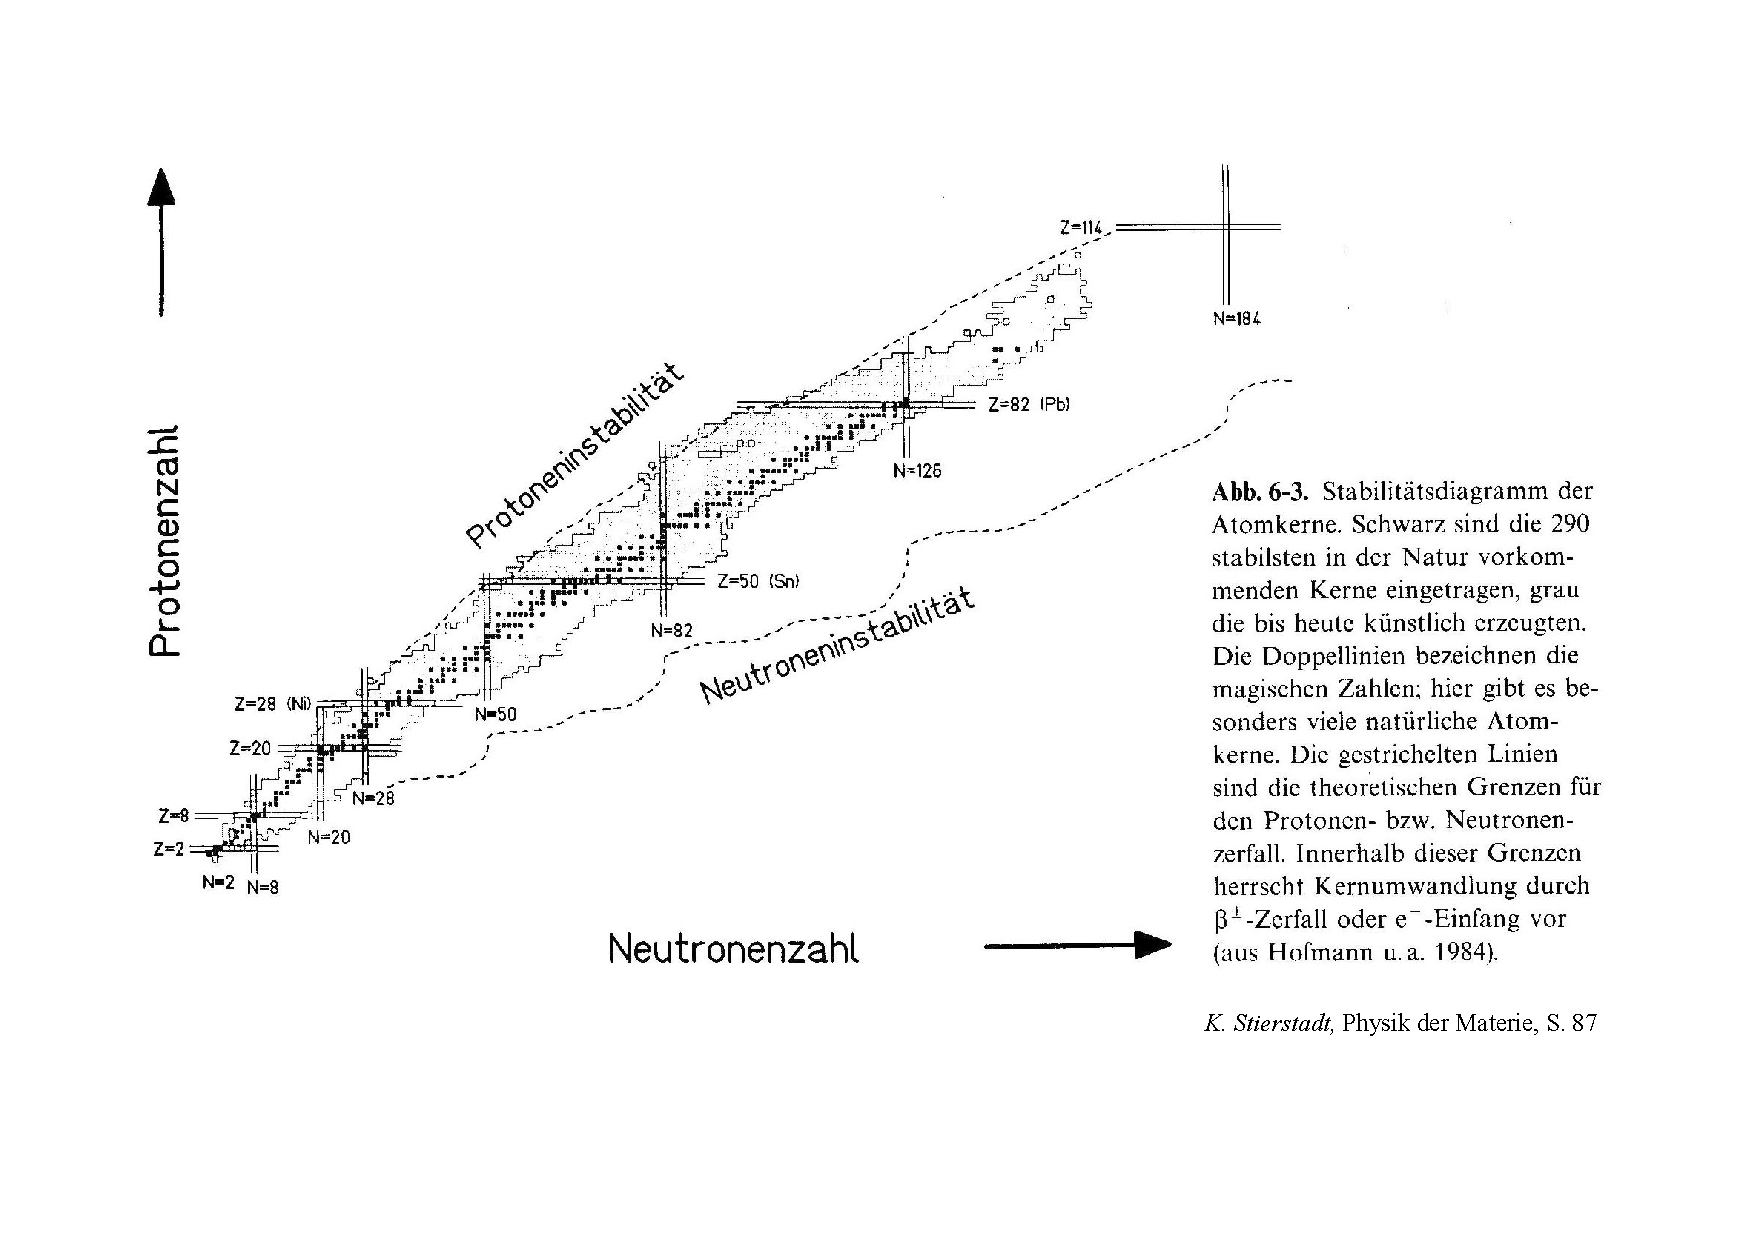
\includegraphics[width=\textwidth]{fig/2-Stabilitaetsdiagramm.pdf}
\end{figure}
\end{enumerate}
%\end{bemn}

\subsubsection{Kernreaktionen}

Wir wollen nun die Bethe-Weizsäcker Formel verwenden, um Aussagen über mögliche
Kernrekationen zu machen. Betrachten wir zunächst den $\alpha$-Zerfall. Die
Energie des $\alpha$-Zerfalls ist
\begin{align*}
E_\alpha =\frac{1}{c^2}
(m(Z,A)-\underbrace{m(Z-2,A-4)-m_\alpha}_{\small\text{Restkern +
$\alpha$ Teilchen}}).
\end{align*}
Falls $E_\alpha < 0$ wird die Teilchenwelle an den Potentialwänden
total reflektiert, durch Interferenz entstehen stehende Wellen. Dies sind
gerade die Eigenzustände des $\alpha$-Teilchens im Potential.

Ist $E_\alpha > 0$ im Potential, so existiert auch ein freier Zustand.
Die Welle wird nun nicht mehr total reflektiert, sondern dringt in die
Potentialwand ein und wird gedämpft. Wir wissen aus der Quantenmechanik,
dass daher das Teilchen eine gewisse Wahrscheinlichkeit hat, die
Potentialbarriere zu überwinden. Die Wahrscheinlichkeit für das Tunneln ist
gegeben durch,
\begin{align*}
&\lambda := \lambda_0\cdot T_\alpha,
\end{align*}
$\lambda_0$ ist die Entstehungswahrscheinlichkeit für das
$\alpha$-Teilchen, $T_\alpha$ bezeichnet den Transmissionskoeffizient.
\begin{align*}
T_\alpha &= \frac{\text{Zahl der erfolgreichen Eindringversuche}}{\text{Zahl
der gesamten Eindringversuche}}\\
&\entspr \text{Verhältnis von einlaufender zu auslaufender Teilchenwelle}.
\end{align*}
Betrachten wir die Wellenfunktionen der einlaufenden und auslaufenden Welle,
können wir den Transmissionkoeffizienten berechnen.
\begin{align*}
T_\alpha = \frac{j_a}{j_e} = \frac{\abs{\Psi_a}^2v_a}{\abs{\Psi_e}^2v_e}.
\end{align*}
Mit $p=mv = \hbar k$ und der Lösung der Wellengleichung für stehende
Wellen
\begin{align*}
\Psi_\nu = \alpha_\nu e^{ik_\nu x} + \beta_n e^{-ik_\nu x},
\end{align*}
erhält man so für das Kastenpotential,
\begin{align*}
T_\alpha = \exp\setd{-\frac{2}{\hbar}\int\limits_0^D \sqrt{2m(V(r)-E)}\dr}.
\end{align*}
Man kann zeigen, dass $T_\alpha$ für beliebige Potentiale diese Form hat.

\subsection{Zerfälle und Radioaktivität}

Über das zeitliche Verhalten von Kernreaktionen lassen sich folgende Aussagen
machen.
\begin{itemize}
  \item Der Zeitpunkt eines Zerfalls kann weder vorhergesagt noch von
  außen beeinflusst werden.
  \item Zerfälle werden durch die Wechselwirkung zwischen den Nukliden
  getrieben.
\end{itemize}
Man kann also nur Aussagen statistischer Natur machen. Wir wollen dies mit
Hilfe von Ratengleichungen tun. Dazu betrachten wir, wie sich eine große
Anzahl $N_0=N(t=0)$ von instabilen Kernen über die Zeit verändert. Sie erfüllt
die Differentialgleichung
\begin{align*}
\frac{\dN}{\dt} = -\Gamma N(t),
\end{align*}
wobei $\Gamma$ die \emph{Zerfallsrate} bezeichnet. Die Lösung dieser Gleichung
ist wohlbekannt,
\begin{align*}
N(t) = N_0 \exp\left(-\Gamma t\right).
\end{align*}
Die \emph{Aktivität} ist definiert als die Anzahl der Ereignisse pro Zeit,
\begin{align*}
A(t) = \abs{\frac{\dN}{\dt}} = N_0 \Gamma \exp\left(-\Gamma t\right).
\end{align*}
Die Aktivität hat also das gleiche Zeitverhalten wie die Anzahl der vorhandenen
Kerne. \textit{A posteriori} scheint dies offensichtlich, dass dem so ist, ist
jedoch eine Besonderheit und im Voraus nicht klar. Aus diesem Zusammenhang kann
man Informationen darüber gewinnen, wie sich die Radioaktivität zeitlich
verhält. Die Einheit der Aktivität ist die SI-Einheit,
\begin{align*}
1 \text{ Becquerel} = 1\mathrm{Bq}.
\end{align*}
\begin{bemn}
Die Aktivität sagt nichts über die Art der Strahlung, deren Energie oder deren
Schädlichkeit für Lebewesen aus.\maphere 
\end{bemn}
Die \emph{mittlere Lebensdauer} eines Kerns erhält man durch,
\begin{align*}
\tau = \frac{\int t\dN}{\int \dN} = \frac{\int t N_0 \Gamma \exp\left(-\Gamma
t\right)\dt}{N_0} = \frac{1}{\Gamma}.
\end{align*}
Die \emph{Halbwertszeit} ist die Zeit, nach der durchschnittlich die Hälfte der
vorhanden Kerne zerfallen ist,
\begin{align*}
&\frac{1}{2} N_0 = N_0 \exp\left(-\Gamma \tau_{1/2}\right)\\
\Leftrightarrow & \ln 2 = \Gamma \tau_{1/2}\\ 
\Leftrightarrow & \tau_{1/2} = \frac{\ln2}{\Gamma}
\end{align*}

In vielen Fällen ist nicht nur ein Zerfall möglich, man spricht dann von
``Zerfallskanälen''. Für ein Nuklid mit 2 Zerfallskanälen gilt,
\begin{align*}
\frac{\dN}{\dt}(t) = -\Gamma_1 N(t) - \Gamma_2 N(t) = -(\Gamma_1+\Gamma_2)N(t).
\end{align*}
Die Gesamtzerfallsrate ist $\Gamma_\text{ges} = \Gamma_1+\Gamma_2$,
Zerfallsraten sind also additiv. Die Halbwertszeit ergibt sich als
\begin{align*}
\tau = \frac{1}{\Gamma_\text{ges}} = \frac{1}{\Gamma_1+\Gamma_2}.
\end{align*}
Die Zeitabhängigkeit der Endprodukte ist
\begin{align*}
&\frac{\dN_i}{\dt} = -\Gamma_i N_i(t),\\
&\frac{N_1(t)}{N_2(t)} = \frac{\Gamma_1}{\Gamma_2}
\end{align*}
Lösungen dieser Gleichungen sind,
\begin{align*}
&N_1(t) = N_0 \frac{\Gamma_1}{\Gamma_1+\Gamma_2}\left(1 -
\exp\left(-\Gamma_\text{ges} t \right)\right)\\
&N_2(t) = N_0 \frac{\Gamma_2}{\Gamma_1+\Gamma_2}\left(1 -
\exp\left(-\Gamma_\text{ges} t \right)\right)
\end{align*}

% 
% \begin{figure}[!htbp]
% 	\centering
% 	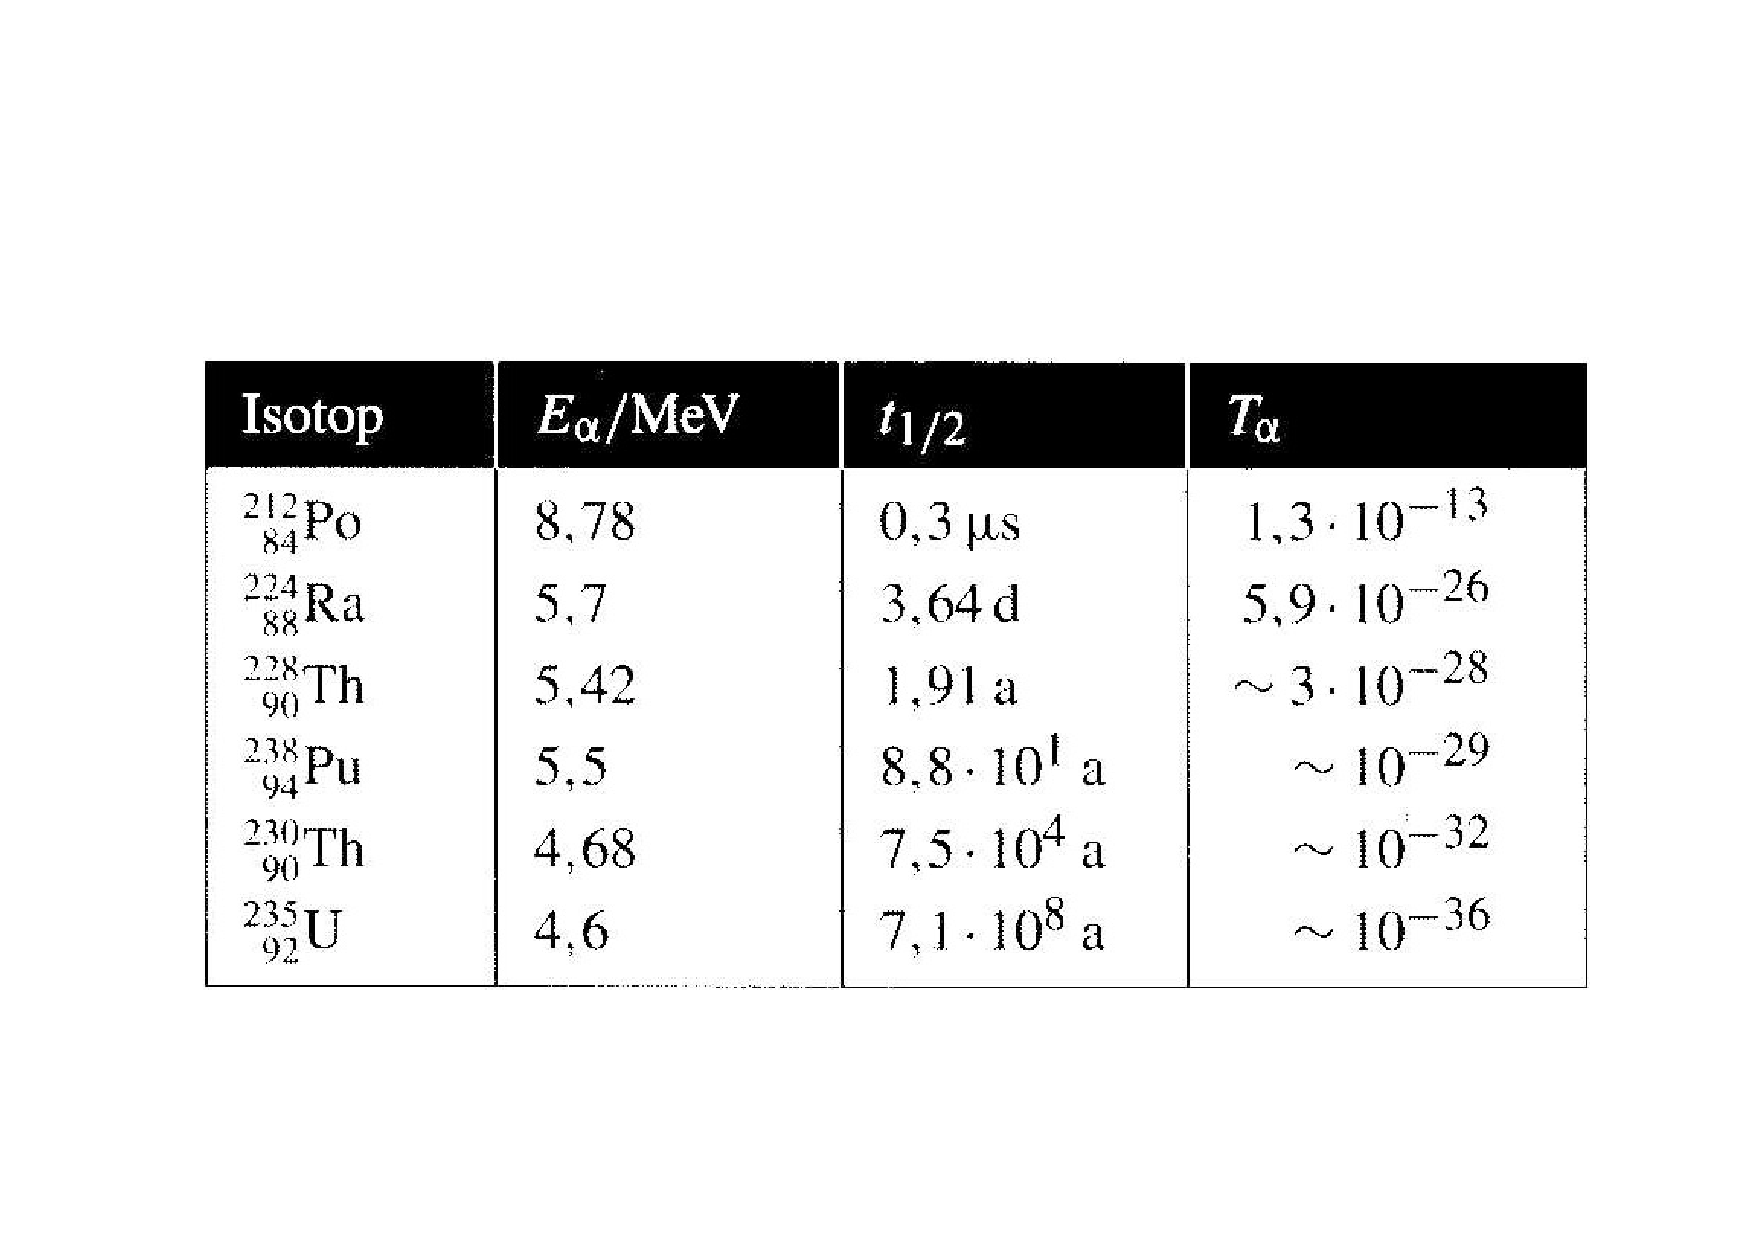
\includegraphics[width=0.9\textwidth]{fig/2-CharakteristischeDatenStrahler.pdf}
% \end{figure}

\sfigure[H][0.9]%
	{2-CharakteristischeDatenStrahler.pdf}
	{\DemtroederFour, S. 46}
	{Charakteristische Daten einiger $\alpha$-Strahler. (Energie $E_\alpha$,
	Halbwertszeit $t_{1/2}$ und Tunnelwahrscheinlichkeit $T_\alpha$)}

\subsubsection{Zusammenfassung}

\textit{$\alpha$-Strahlung} hat ein diskretes Spektrum, da die Anregungszustände
der Kerne diskret sind. Sie tritt dann auf, wenn durch die Abspaltung eines
$\alpha$-Teilchens die Bindungsenergie vergrößert werden kann. Da das
$\alpha$-Teilchen eine sehr hohe Bindungsenergie hat, wird dieser Zerfall
gegenüber der Abspaltung von einzelnen $p^+$, $n^0$ bevorzugt.

\textit{$\beta$-Strahlung} hat ein kontinuierliches Spektrum. Es handelt sich
hier um einen 3-Körper-Prozess, weshalb die Energie kontinuierlich verteilt
werden kann.
\begin{align*}
&n^0 \to p^+ + e^- + \overline{\nu}_e\\
&p^+ \to n^0 + e^+ + \nu_e
\end{align*}
Beim Zerfall entstehen die Spin-$\frac{1}{2}$-Teilchen Elektronneutrino $\nu_e$
bzw. Elektronantineutrino $\overline{\nu}_e$ aufgrund der
Impuls- und Drehimpulserhaltung.

\textit{$\gamma$-Strahlung} entsteht bei ``optischen Übergängen'' von
angeregten Kernzuständen. Hierbei werden Photonen im $\mathrm{MeV}$-Bereich
emittiert. Typischerweise folgt auf einen $\alpha$-/$\beta$-Zerfall ein
$\gamma$-Zerfall, da die Zerfallsprodukte bei letzteren in angeregten
Zuständen zurückbleiben.

Aus der Paritätsregel und der Drehimpulserhaltung erhalten wir Auswahlregeln
für diese Übergänge. Dipolstrahlung im Fall von $\Delta L = 1$,
Quadrupolstrahlung für $\Delta L = 2$.

\subsubsection{Andere Strahlungseinheiten}
Wird ein lebender Organismus Strahlung ausgesetzt, kann man mithilfe der
\emph{Dosis} Aussagen über die Auswirkungen machen,
\begin{align*}
&\nrm{D} = \nrm{\frac{\text{absorbierte Energie}}{\text{Masse}}} = 1
\frac{\mathrm{J}}{\mathrm{kg}} = 1 \mathrm{Gray} = 1 \mathrm{Gy}\\
&\nrm{\dot{D}} = \frac{\mathrm{Gy}}{\mathrm{s}}.
\end{align*}
Die Schädlichkeit der Strahlung an sich wird durch die \emph{Äquivalentdosis}
\begin{align*}
H=Q\cdot D,\qquad \text{Einheit }S_V\text{ (Sievert)},
\end{align*}
beschrieben, wobei $Q$ einen Qualitätsfaktor darstellt.

%\begin{table}[h]
\begin{tabular}[h]{l|c}
 & $Q$\\\hline
 $\gamma/\beta$-Strahlung & 1\\
 thermische Neturonen $n_\tau$ & 2.3\\
 schnelle Neutronen $n_S$ & 10\\
 $\alpha$-Strahlung & 20
\end{tabular}
%\end{table}
